\documentclass{article}

\usepackage[utf8]{inputenc}

\title{Formalisms\\
Every Computer Scientist Should Know}
\date{}
% \newcommand{\booklicense}{
%     This work is marked with CC0 1.0. 
%     To view a copy of this license, visit http://creativecommons.org/publicdomain/zero/1.0
% }

% Author subtitle
% For example, university or geographical location
% \newcommand{\authorsubtitle}{ISTA}


\synctex=1

% PACKAGES

% this package allows large \fontsize
\usepackage{fix-cm}  
% this is for graphics. e.g. rectangle on title page
\usepackage{tikz}    
% Used by equations
\usepackage{amsmath} 
\usepackage{amssymb,amsfonts,amsthm,mathtools}
\usepackage[shortlabels]{enumitem}

% Paper dimensions
% \usepackage[a4paper, total={6in, 8in}]{geometry}
% Inserting images
\usepackage{graphicx}
% Index creation
\usepackage{makeidx}
% Initialize an index so we can add entries with \index
\makeindex 
% Others
\usepackage{pbox}
\usepackage{stmaryrd}
% Links
\usepackage{hyperref}
% Convenient references
\usepackage{cleveref}
% Derivations written using horizontal lines
\usepackage{mathpartir}
% TikZ figures
\usepackage{tikz}
% algorithms
\usepackage{algorithm}
\usepackage{algpseudocode}
% proof systems
\usepackage{bussproofs}

\usetikzlibrary {petri}
\usetikzlibrary{arrows.meta}
\usetikzlibrary{shapes,snakes}
\usetikzlibrary{fit}


\theoremstyle{plain}
\newtheorem{theorem}{Theorem}[section]
\newtheorem{lemma}[theorem]{Lemma}
\newtheorem{corollary}[theorem]{Corollary}

\theoremstyle{definition}
\newtheorem{definition}{Definition}[section]
\newtheorem{exercise}{Exercise}[section]
\newtheorem{example}{Example}[section]

\theoremstyle{remark}
\newtheorem{remark}{Remark}[section]
\newtheorem{metatheorem}{Metatheorem}[section]
\newtheorem{axiom}{Axiom}[section]

\DeclareMathOperator{\lub}{lub}
\DeclareMathOperator{\glb}{glb}



%%%%%% Basic Math
\newcommand{\comment}[1]{\textcolor{red}{#1}}

\newcommand{\notimplies}{%
  \mathrel{{\ooalign{\hidewidth$\not\phantom{=}$\hidewidth\cr$\implies$}}}}


\newcommand{\RN}{\mathbb{R}}
\newcommand{\QN}{\mathbb{Q}}
\newcommand{\NN}{\mathbb{N}}
\newcommand{\BN}{\mathbb{B}}
\newcommand{\ZN}{\mathbb{Z}}
\newcommand{\power}{\mathcal{P}}

\newcommand{\true}{\mathbf{true}}
\newcommand{\false}{\mathbf{false}}


\newcommand{\simplies}{\Rightarrow}
\newcommand{\simplied}{\Leftarrow}
\newcommand{\siff}{\Leftrightarrow}
\newcommand{\emptystring}{\epsilon}
\newcommand{\gfp}{\mathrm{gfp}}
\newcommand{\lfp}{\mathrm{lfp}}
\newcommand{\bottom}{\perp}

\newcommand{\valfoo}{\nu}
\newcommand{\eval}[1]{\llbracket #1 \rrbracket}
\newcommand{\interp}{\mathcal{I}}

\newcommand{\sat}{\mathbf{sat}}
\newcommand{\unsat}{\mathbf{unsat}}
%%%%%% Merge Sort

\newcommand{\mergesort}{\mathtt{mergesort}}
\newcommand{\merges}{\mathtt{merge}}
\newcommand{\odd}{\mathtt{odd}}
\newcommand{\even}{\mathtt{even}}
\newcommand{\sorted}{\mathtt{sorted}}
\newcommand{\reverseA}{\mathtt{reverse}}
\newcommand{\reverseB}{\mathtt{reverse2}}

\newcommand{\parent}{\mathtt{parent}}
\newcommand{\monkey}{\mathtt{monkey}}
\newcommand{\human}{\mathtt{human}}


\newcommand{\proofs}{\vdash}


\newcommand{\hilbert}{\mathcal{H}}
% \newcommand{\nj}{\mathcal{N}\mkern-9mu\mathcal{J}}
% \newcommand{\nk}{\mathcal{N}\mkern-6mu\mathcal{K}}
% \newcommand{\lk}{\mathcal{L}\mkern-6mu\mathcal{K}}
\newcommand{\nj}{\mathcal{NJ}}
\newcommand{\nk}{\mathcal{NK}}
\newcommand{\lk}{\mathcal{LK}}
 
\newcommand{\kripke}{m}
\newcommand{\krel}{\preceq}
\newcommand{\kinit}{w_0}
\newcommand{\kworld}{W}


\newcommand{\lif}{\mathrm{if}}
% \newcommand{\ln}{\underline{if}}


\newcommand{\tuple}[1]{\langle #1 \rangle}

\newcommand{\sif}[3]{\mathrm{if}\;#1\;\mathrm{then}\;#2\;\mathrm{else}\;#3}
\newcommand{\swhile}[2]{\mathrm{while}\;#1\;\mathrm{do}\;#2}
\newcommand{\siffi}[1]{\mathrm{if}\;#1\;\mathrm{fi}}
\newcommand{\sdo}[1]{\mathrm{do}\;#1\;\mathrm{od}}
\newcommand{\sskip}{\mathtt{skip}}
\newcommand{\sassert}{\mathtt{assert}}
\newcommand{\sfail}{\mathtt{fail}}
\newcommand{\sassume}{\mathtt{assume}}
\newcommand{\sabort}{\mathtt{abort}}
\newcommand{\ssc}{\mathtt{c}}
\newcommand{\ssb}{\mathtt{b}}
\newcommand{\sgc}{\mathtt{gc}}

\newcommand{\simp}[1]{\mathtt{#1}}
\newcommand{\sop}[2]{\langle \simp{#1},~#2 \rangle}
\newcommand{\sde}[1]{\llbracket \simp{#1} \rrbracket}
\newcommand{\sdefun}[1]{\lambda \sigma.~ #1}

\newcommand{\imp}[1]{\texttt{#1}}
\newcommand{\opsem}[2]{\langle \imp{#1},~#2 \rangle}
\newcommand{\desem}[1]{\llbracket \imp{#1} \rrbracket}
\newcommand{\defun}[1]{\lambda \sigma.~ #1}



\newcommand{\vc}{\mathrm{vc}}
\newcommand{\wlp}{\mathrm{wlp}}
\newcommand{\wsp}{\mathrm{wp}}



\newcommand{\ccs}{\mathcal{P}}

\newcommand{\coin}{\;\mathrm{coin}\,}
\newcommand{\discof}{\;\mathrm{discof}\,}
\newcommand{\reqcof}{\;\mathrm{reqcof}\,}
\newcommand{\distea}{\;\mathrm{distea}\,}
\newcommand{\reqtea}{\;\mathrm{reqtea}\,}


\newcommand{\inc}{\;\mathrm{inc}\,}
\newcommand{\dec}{\;\mathrm{dec}\,}
\newcommand{\zero}{\;\mathrm{zero}\,}
\newcommand{\Counter}{\;\mathrm{Counter}\,}
\newcommand{\semicounter}{\;\mathrm{Semicounter}\,}



\newcommand{\equiso}{\approx_{\mathrm{iso}}}
\newcommand{\equbis}{\approx_{\mathrm{bis}}}
\newcommand{\equsim}{\approx_{\mathrm{sim}}}
\newcommand{\equlin}{\approx_{\mathrm{lin}}}

\newcommand{\lequsim}{\preceq_{\mathrm{sim}}}
\newcommand{\gequsim}{\succeq_{\mathrm{sim}}}

\providecommand{\T}{T}
\DeclareMathOperator{\pre}{pre}
\DeclareMathOperator{\post}{post}
\DeclareMathOperator{\HML}{HML}
\DeclareMathOperator{\HMLlin}{HML_{\mathrm{lin}}}



\newcommand{\bev}[1]{\langle #1 \rangle}
\newcommand{\bal}[1]{[ #1 ]}

\newcommand{\lev}{\lozenge}
\newcommand{\lal}{\square}
\newcommand{\lne}{\bigcirc}
\newcommand{\lun}{\,\mathcal{U}\,}

\newcommand{\lmu}{\mu\,}
\newcommand{\lnu}{\nu\,}

\newcommand{\algo}{\mathcal{A}}


\newcommand{\tatom}{\mathrm{atom}}
\newcommand{\tcar}{\mathrm{car}}
\newcommand{\tcdr}{\mathrm{cdr}}
\newcommand{\tcons}{\mathrm{cons}}

\newcommand{\tread}{\mathrm{read}}
\newcommand{\twrite}{\mathrm{write}}


\begin{document}
\maketitle
\addcontentsline{toc}{chapter}{Index}
% \include{title}

% \section{Tools}
% \begin{itemize}
%   \item Lean or Coq 
%   \item CVC5 or Z3 
%   \item possibly a model checker 
%   \item professional version of ChatGPT
% \end{itemize}

% \section{Syllabus}
% \begin{enumerate}
%   \item MATH (``Informalism'')
%   \begin{itemize}
%     \item proofs (natural deduction)
%     \item fixpoints (induction, coinduction)
%   \end{itemize}
%   \item DECLARATIVE LOGIC
%   \begin{itemize}
%     \item syntax (rules) vs. semantics (models)
%     \item propositional, predicate, modal logic 
%     \item decision procedures (SAT, SMT)
%   \end{itemize}
%   \item FUNCTIONS
%   \begin{itemize}
%     \item $\lambda$ calculus, typed $\lambda$
%     \item SOS (structured operational semantics), rewriting
%     \item ``propositions-as-types'' (connection to logic)
%   \end{itemize}
%   \item PROCESSES (CONCURRENT)* 
%   \begin{itemize}
%     \item CCS, Petri nets
%     \item (bi-) simulation
%   \end{itemize}
%   \item CIRCUITS*
%   \begin{itemize}
%     \item boolean, sequential, dataflow (Kahn nets)
%     \item interfaces
%   \end{itemize}
%   \item STATE TRANSITION SYSTEMS*
%   \begin{itemize}
%     \item ($\omega$-) automata, games, timed, probabilistic, pushdown
%     \item programs, Turing machines 
%     \item grammars (Chomsky hierarchy)
%   \end{itemize} 
%   \item DECLARATIVE SPECIFICATION
%   \begin{itemize}
%     \item Hoare logics, separation logic 
%     \item temporal logics (LTL, CTL, ATL)
%     \item partial correctness vs. termination, safety vs. liveness 
%   \end{itemize}
% \end{enumerate}

% *: Operational.

\section{Lecture 1: How to write an informal proof}

\subsection{Example 1: Sum of two bounded functions}

\begin{definition}
  A real number $b \in \RN$ is a \emph{bound} of a 
  function $f\colon \RN\to \RN$ from $\RN$ to $\RN$, if for all $x$ in 
  $\RN$, we have $f(x) \leq b$. 
\end{definition}


\begin{definition}
  Given two functions $f\colon  \RN\to \RN$ and $g\colon  \RN\to \RN$ from $\RN$ to $\RN$, their \emph{sum} is the function $f + g$ such 
  that for all $x$ in $\RN$, we have $(f+g) (x) = f(x) + g(x)$.
\end{definition} 


\begin{theorem}
  For all functions $f\colon  \RN\to \RN$ and $g\colon  \RN\to \RN$, if $f$ and
  $g$ are bounded, then $f+g$ is bounded. 
\end{theorem}
\begin{proof}
Consider arbitrary functions $\hat{f}$ and $\hat{g}$ from $\RN$ to $\RN$.
We assume that $\hat{f}$ and $\hat{g}$ are bounded, and want to 
show that $\hat{f} + \hat{g}$ is bounded.

By the definition of boundedness, we show that there exists a $b \in \RN$ such
that for all $x \in \RN$, $(\hat{f} + \hat{g})(x) \leq b$.

For this, let $\hat{b_1}$ be such that for all $x \in \RN$, $\hat{f}(x) \leq \hat{b_1}$.
Similarly, let $\hat{b_2}$ be a bound for $\hat{g}$.
We show that $\hat{b_1} + \hat{b_2}$ is a bound for $\hat{f} + \hat{g}$, i.e.
for all $x \in \RN$, we have $(\hat{f} + \hat{g})(x) \leq \hat{b_1} + \hat{b_2}$.

Consider an arbitrary $\hat{x} \in \RN$. We show that $(\hat{f} + \hat{g})(\hat{x}) \leq \hat{b_1} + \hat{b_2}$.
By the definition of + for functions, we have to show $\hat{f}(\hat{x}) + \hat{g}(\hat{x}) \leq \hat{b_1} + \hat{b_2}$.

For all $x_1, x_2, y_1, y_2 \in \RN$, if $x_1 \leq y_1$ and $x_2 \leq y_2$, then $x_1 + x_2 \leq y_1 + y_2$. 
This can be broken down even further:

\begin{enumerate}
  \item[(i)] for all $x,y,z \in \RN$, if $x \leq y$ and $y \leq z$, then $x \leq z$
  \item[(ii)] for all $x,y \in \RN$, $x + y = y + x$
  \item[(iii)] for all $x,y,z \in \RN$, if $x \leq y$, then $x + z \leq y + z$
\end{enumerate}
\end{proof}

\subsection{Example 2: Schröder-Bernstein Theorem}

\begin{definition}
  Two sets $A$ and $B$ are \emph{equipollent} (``have the same 
  size''), if there is a bijection from $A$ to $B$.
\end{definition}

\begin{definition}
  A function $f$ from $A$ to $B$ is: 
  (i) \emph{one-to-one} if for all $x$ and $y$ in $A$, if $x \neq y$, then $f(x) \neq f(y)$;
  (ii) \emph{onto} if for all $z$ in $B$, there exists $x$ 
    in $A$ such that $f(x) = z$;
(iii) \emph{bijective} if $f$ is one-to-one and onto.
\end{definition}




% \begin{center}
% \begin{tabular}{
%   p{0.35\linewidth} | p{0.35\linewidth} | p{0.2\linewidth}}
%   Goals & Knowledge & Outermost symbol \\
%   \hline
%   \begin{itemize}[leftmargin=*]
%     \item[] Show for all $x$, $G(x)$.
%     \item[] Consider arbitrary $\hat{x}$.
%     \item[] Show $G(\hat{x})$. 
%   \end{itemize} & \begin{itemize}[leftmargin=*]
%     \item[] We know for all $x$, $K(x)$.
%     \item[] In particular, we know $K(\hat{t})$.
%     \item[] $\hat{t}$: term containing only constants. 
%   \end{itemize} & \begin{itemize}
%     \item[] \Large $\forall$
%   \end{itemize} \\ 
%   \hline 
%   \begin{itemize}[leftmargin=*]
%     \item[] Show there exists $x$ s.t. $G(x)$.
%     \item[] We show that $G(\hat{t})$.
%     \item[] $\hat{t}$: term containing only constants.
%   \end{itemize} & \begin{itemize}[leftmargin=*]
%     \item[] We know there exists $x$ s.t. $K(x)$.
%     \item[] Let $\hat{x}$ be s.t. $K(\hat{x})$.
%   \end{itemize} & \begin{itemize}
%     \item[] \Large $\exists$
%   \end{itemize}
% \end{tabular}
% \end{center}

\begin{theorem}[Schr\"{o}der-Bernstein theorem]
    \label{thrm:class1:bernstein}
    If there is a one-to-one function on a set $A$ to a subset of a set $B$ and
    there is also a one-to-one function on $B$ to a subset of $A$, then $A$ and
    $B$ are equipollent.
\end{theorem}

\begin{exercise}
    Correct the following incorrect proof of Theorem \ref{thrm:class1:bernstein} \emph{in the presented style}:
    \begin{quote}
Suppose that $f$ is a one-to-one map of $A$ into $B$ and $g$ is
one-to-one on $B$ to $A$. It may be supposed that $A$ and $B$ are disjoint. The proof of the theorem is accomplished by decomposing $A$ and $B$ into classes which are most easily described in terms of parthenogenesis. A point $x$ (of either $A$ or $B$) is an ancestor of a point $y$ iff $y$ can be obtained from $x$ by successive application of $f$ and $g$ (or $g$ and $f$). Now decompose $A$ into three sets:
let $A_e$ consist of all points of $A$ which have an even number of ancestors, let $A_o$ consist of points which have an odd number of ancestors, and let $A_{\infty}$ consist of points with infinitely many ancestors. Decompose $B$ similarly and observe: f maps $A_e$ onto
$B_o$ and $A_{\infty}$ onto  $B_{\infty}$, and $g^{-1}$ maps $A_o$ onto $B_e$. Hence the function which agrees with $f$ on $A_e\cup A_{\infty}$, and agrees with $g^{-1}$ on $A_o$ is a one-to-one map of $A$ onto $B$.
    \end{quote}
\end{exercise}

\newpage

\section{Lecture 2}

\subsection{Style Guide}
We provide an informal style guide for writing mathematical proofs. 

\begin{center}
    \begin{tabular}{l|l|c}
     Goal & Knowledge & \shortstack[c]{Outermost\\symbol} \\
    \hline 
        \pbox{20cm}{Show for all $x$, $G(x)$. \\ Consider arbitrary $\hat{x}{}^1$.\\ Show $G(\hat{x})$}
      & \pbox{20cm}{We know for all $x$, $K(x)$ \\ In particular we know $K(\hat{t}){}^2$}
      & $\forall$ \\
    \hline 
        \pbox{20cm}{Show: exists $x$ s.t. $G(x)$. \\ We show $G(\hat{t}){}^2$}
      & \pbox{20cm}{We know exists $x$ s.t. $K(x)$ \\ Let $\hat{x}{}^1$ be s.t. $K(\hat{x})$}
      & $\exists$ \\
    \hline
        \pbox{20cm}{Show if $G_1$ then $G_2$ \\ Assume $G_1$\\ Show $G_2$}
      & \pbox{20cm}{We know if $K_1$ then $K_2$\\ To show $K_2$ it suffices to show $K_1$\\ Know $K_1$, Also know $K_2$}
      & $\Rightarrow$ \\
    \hline
        \pbox{20cm}{Show $G_1$ iff $G_2$ \\ 1. Show if $G_1$ then $G_2$\\ 2. Show if $G_2$ then $G_1$}
      & \pbox{20cm}{We know $K_1$ iff $K_2$\\ In particular we know if $K_1$ then $K_2$\\ and if $K_2$ then $K_1$}
      & $\iff$ \\
    \hline
        \pbox{20cm}{Show $G_1$ and $G_2$\\ 1. Show $G_1$, \textbf{and}\\ 2. Show $G_2$}
      & \pbox{20cm}{Know $K_1$ and $K_2$\\ Also Know $K_1$ \\ Also Know $K_2$}
      & $\wedge$ \\
    \hline
        \pbox{20cm}{Show $G_1$ or $G_2$\\ Either, assume $\neg G_1$, show $G_2$, \textbf{or}\\ Assume $\neg G_2$, show $G_1$}
      & \pbox{20cm}{We know $K_1$ or $K_2$. Show $G$.\\ case 1: Assume $K_1$, Show $G$\\ case 2: Assume $K_2$, Show $G$ \\ Case split $\uparrow$}
      & $\vee$ \\
    \hline
     \multicolumn{2}{c|}{\pbox{20cm}{Move Negation Inside, as far as possible}} &  $\neg$ \\ 
    \hline
     \multicolumn{3}{c}{$\rule{0pt}{1.5em} {}^1$ where $\hat{x}$ is a new constant.\hspace{2em} ${}^2$ where $\hat{t}$ is any constant expression}
\end{tabular}
\end{center}


\subsection{Lattices and Fixpoints}
We define relations and their properties. 

\begin{definition}[Relation]
A binary \emph{relation} $R$ on a set $A$ is a subset $R \subseteq A\times A$.
The relations $R$ is:
\begin{itemize}
    \item \emph{reflexive} if for all $x$ in $A$, we have $R(x,x)$.
    \item \emph{anti-symmetric} if for all $x$ and $y$ in $A$, if $R(x,y)$ and $R(y,x)$ then $x=y$.
    \item \emph{transitive} if for all $x,y$ and $z$ in $A$, if $R(x,y)$ and $R(y,z)$ then $R(x,z)$.
    \item a \emph{partial order} if $R$ is reflexive, anti-symmetric and transitive.
\end{itemize}
\end{definition}

\begin{definition}[poset]
     A \emph{poset} $(A,\sqsubseteq)$ is a set $A$ and a partial order $\sqsubseteq$ on $A$.
\end{definition}


\begin{example}
    Let $\NN$ be the natural numbers. The pair $(\NN,\leq)$ is a poset.
\begin{center}
     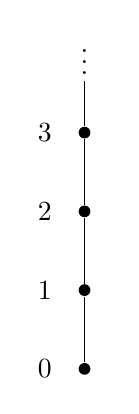
\begin{tikzpicture}[scale=1, every node/.style={circle, fill, inner sep=1.5pt}, 
    label distance=2mm]

    % Nodes
    \node[label=left:{$0$}] (0) at (0, 0) {};
    \node[label=left:{$1$}] (1) at (0 ,1) {};
    \node[label=left:{$2$}] (2) at (0, 2) {};
    \node[label=left:{$3$}] (3) at (0, 3) {};
   \node[draw=none, fill=none] (4) at (0,4) {$\vdots$};  % Dots to indicate continuation
   
    % Lines
    \draw (0) -- (1);
    \draw (1) -- (2);
    \draw (2) -- (3);
    \draw (3) -- (4);

\end{tikzpicture}
 \end{center}
\end{example}

% \begin{example}
   
   
%     \begin{figure}[h]
%         \centering
%         \includegraphics[width=0.7\linewidth]{images/poset.png}
%     \end{figure}
% \end{example}


\begin{example}
 For any set $B$ let $\power(B)$ be the powerset.
 The pair $(\power(B),\subseteq)$ is a poset. E.g., for $B\coloneqq \{a\}$ (left) and for $B \coloneqq \{a,b\}$ (right).
 \begin{center}
 
     \begin{tikzpicture}[scale=1, every node/.style={circle, fill, inner sep=1.5pt}, 
    label distance=2mm]

     \node[label=right:{$\emptyset$}] (0) at (-6,0 ) {};
    \node[label=right:{$\{a\}$}] (1) at (-6,2 ) {};
    % Nodes
    \node[label=right:{$\emptyset$}] (emptyset) at (0, 0) {};
    \node[label=left:{$\{a\}$}] (a) at (-1, 1) {};
    \node[label=right:{$\{b\}$}] (b) at (1, 1) {};
    \node[label=right:{$\{a,b\}$}] (ab) at (0, 2) {};
    
    % Lines
    \draw (0) -- (1);
    
    \draw (emptyset) -- (a);
    \draw (emptyset) -- (b);
    \draw (a) -- (ab);
    \draw (b) -- (ab);

\end{tikzpicture}
 \end{center}

\end{example}

\begin{definition}[Upper Bound]
    Let $(A,\sqsubseteq)$ be a poset. Then (i) $x$ in $A$ is an \emph{upper bound} of a subset $B$ of $A$ if for all $y$ in $B$, it holds that $y \sqsubseteq x$;
    (ii) $x$ is the \emph{least upper bound} (lub) of $B$ if $x$ is an upper bound of $B$ and for all upper bounds $y$ of $B$, we have $x \sqsubseteq y$. %We denote such $x$ by $\bigsqcup B$.
\end{definition}

\begin{definition}[Lower Bound]
    Let $(A,\sqsubseteq)$ be a poset. Then (i) $x$ in $A$ is a \emph{lower bound} of a subset $B$ of $A$ if for all $y$ in $B$, it holds that $x \sqsubseteq y$;
    (ii) $x$ is the \emph{greatest lower bound} (glb) of $B$ if $x$ is a lower bound of $B$ and for all lower bounds $y$ of $B$, we have $y \sqsubseteq x$. %We denote such $x$ by $\bigsqcap B$.
\end{definition}

\begin{example}
    Consider the poset $(\NN,\leq)$. Then for any $B \subseteq \NN$, if $B$ is finite, $\lub(B)$ is well-defined and equal to $\max(B)$. If $B$ is infinite, then $\lub(B)$ does not exist.
\end{example}

\begin{example}
   Consider the poset $(\NN \cup \{\infty\},\leq)$ where for all $x$ in $\NN$, it holds that $x \leq \infty$. Then for all $B \subseteq \NN$, $\lub(B)$ is well-defined.
\end{example}

\begin{example}
    Let $A$ be any set and consider the poset $(\power(A),\subseteq)$. For any subset $B$ of $\power(A)$, it holds that $\lub(B) = \bigcup B$ and $\glb(B) = \bigcap B$.
\end{example}

\begin{lemma}
  Let $(A,\sqsubseteq)$ be a poset. For all $x$, $y$ in $A$, and any subset $B$ of $A$, if $x$ and $y$ are lubs (glbs) of $B$, then $x = y$.
\end{lemma}

\begin{proof}
    Consider arbitrary $\hat{x}, \hat{y} \in A$ and $\hat B \subseteq A$. Assume $\hat x$ is a lub of $\hat B$
    and $\hat y$ is a lub of $\hat B$. We know:
    \begin{enumerate}
        \item[(i)] for all $z \in B$, $z \sqsubseteq \hat{x}$,
        \item[(ii)] for all $z \in B$, $z \sqsubseteq \hat{y}$,
        \item[(iii)] for all $z \in A$, if $z$ is an upper bound of $B$ then
        $\hat x \sqsubseteq z$ and
        \item[(iv)]for all $z \in A$, if $z$ is an upper bound of $B$ then $\hat
        y \sqsubseteq z$.
    \end{enumerate}
    From (ii) we know that $\hat{y}$ is an upper bound, and therefore, by (iii), $\hat{x} \sqsubseteq \hat{y}$. Symmetrically, by (i) and (iv) we get $\hat{y} \sqsubseteq \hat{x}$. By antisymmetry, $x = y$.
\end{proof}

Given that the \emph{least upper bound} and the \emph{greatest lower bound} are unique (if they exist), for any set $A$ and $B \subseteq A$, we write $\bigsqcup B$ to denote $\lub(B)$ and $\bigsqcap B$ to denote $\glb(B)$.

\begin{definition}[Lattice]
    A poset $(A,\sqsubseteq)$ is a \emph{lattice} if for all $x$, $y$ in $A$, the lub $\bigsqcup \{x,y\}$ ($x \sqcup y$, join) and the glb $\bigsqcap \{x,y\}$ ($x \sqcap y$, meet) exist.
\end{definition}

\begin{definition}[Complete Lattice]
    A poset $(A,\sqsubseteq)$ is a \emph{complete lattice} if for all $B \subseteq A$, the lub $\bigsqcup B$ and glb $\bigsqcap B$ exist.
\end{definition}

\begin{example}
    Let $(A,\sqsubseteq)$ be a complete-lattice. Then: $\bigsqcup A = \top$, $\bigsqcap A = \bot$, $\bigsqcup \varnothing = \bot$, and $\bigsqcap \varnothing = \top$. $\top$ and $\bot$ are called top and bottom, respectively.
\end{example}

\begin{definition}[Monotone Function]
Let $(A, \sqsubseteq)$ be a poset. A function $F: A \to A$ is \emph{monotone} if for all $x$, $y$ in $A$, if $x \sqsubseteq y$ then $F(x) \sqsubseteq F(y)$.
\end{definition}

\begin{definition}
Let $(A, \sqsubseteq)$ be a poset and $F: A \to A$. An element $x$ in $A$ is,
\begin{enumerate}
  \item a \emph{prefixpoint} of $F$ if $x \sqsubseteq F(x)$,
  \item a \emph{postfixpoint} of $F$ if $F(x) \sqsubseteq x$.
\end{enumerate}
\end{definition}

% TODO
\begin{definition}[Fixpoint]
Let $(A, \sqsubseteq)$ be a poset and $F: A \to A$. An element $x$ in $A$ is a \emph{fixpoint} of $F$ if it is both a \emph{pre-} and \emph{postfixpoint} of $F$.
\end{definition}

\begin{theorem}[Knaster-Tarski]
\label{thrm:knaster}
    Let $(A,\sqsubseteq)$ be a complete lattice and let $F$ a monotone function on $A$.
    Further, let $\hat{y} = \{x \mid x \sqsubseteq F(x)\}$ and $\hat{z} = \{x \mid F(x) \sqsubseteq x\}$.
    It holds, that:
    \begin{enumerate}
      \item $\hat{y}$ and $\hat{z}$ are fixpoints of $F$,
      \item for all fixpoints $x$ of $F$, $\hat{y} \sqsubseteq x \sqsubseteq \hat{z}$
    \end{enumerate}
\end{theorem}

{\flushleft We write $\lfp(F) = \bigsqcap\{x \mid F(x)\sqsubseteq x\}$ and $\gfp(F) = \bigsqcup\{x \mid x \sqsubseteq F(x)\}$, to denote the least fixpoint and the greatest fixpoint, respectively.}

\begin{exercise}
        Prove the Knaster Tarski Theorem (Theorem \ref{thrm:knaster}).
\end{exercise}



\section{Lecture 3}
\subsection{Kleene Fixed-Point Theorem}
\begin{definition}[$\bigsqcup$-continuous]
    Consider a complete lattice $(A, \sqsubseteq)$.
	A function $f \colon A \to A$ is $\bigsqcup$-continuous if, for all increasing sequences $x_0 \sqsubseteq x_1 \sqsubseteq x_2 \sqsubseteq x_2 \sqsubseteq \ldots$, we have
    \begin{align*}
        f \left( \bigsqcup \{ x_n : n \in \NN \} \right) = \bigsqcup \{ f(x_n) : n \in \NN \} \,.
    \end{align*}
\end{definition}


\begin{definition}[$\bigsqcap$-continuous]
    Consider a complete lattice $(A, \sqsubseteq)$.
	A function $f \colon A \to A$ is $\bigsqcap$-continuous if, for all increasing sequences $x_0 \sqsupseteq x_1 \sqsupseteq x_2 \sqsupseteq x_2 \sqsupseteq \ldots$, we have
 \begin{align*}
     	f \left( \bigsqcap \{ x_n : n \in \NN \} \right) = \bigsqcap \{ f(x_n) : n \in \NN \} \,.
 \end{align*}
\end{definition}

\begin{lemma}
    Both $\bigsqcup$-continuous and $\bigsqcap$-continuous imply monotonicity respectively. 
\end{lemma}


\begin{exercise}
    Let $f \colon A \to A$ be a monotone function. Is one of the two following statements true?
    \begin{enumerate}
        \item For every sequence $x_0 \sqsubseteq x_1 \sqsubseteq x_2 \sqsubseteq x_3 \sqsubseteq \ldots$, we have
        \[
        f \left( \bigsqcup \{ x_n : n \in \NN \} \right) \sqsubseteq \bigsqcup \{ f(x_n) : n \in \NN \}.
        \]

        \item For every sequence $x_0 \sqsubseteq x_1 \sqsubseteq x_2 \sqsubseteq x_3 \sqsubseteq \ldots$, we have
        \[
        f \left( \bigsqcap \{ x_n : n \in \NN \} \right) \sqsupseteq \bigsqcap \{ f(x_n) : n \in \NN \}.
        \]
    \end{enumerate}
\end{exercise}



\begin{theorem}[Constructive Fixed-Point, Kleene's Fixed-Point]
    \label{thrm:constructive-fixedpoints}
    Consider a complete lattice $(A, \sqsubseteq)$. Then, for every $\bigsqcup$-continuous function $f \colon A \to A$, we have
    \[
    \lfp f = \bigsqcup \{ f^n(\bot) : n \in \mathbb{N} \},
    \]
    and for every $\bigsqcap$-continuous function $f \colon A \to A$, we have
    \[
    \gfp f = \bigsqcap \{ f^n(\top) : n \in \mathbb{N} \}.
    \]
\end{theorem}    


\begin{exercise}
    Prove the Constructive Fixed-Point Theorem (Theorem \ref{thrm:constructive-fixedpoints})
\end{exercise}
	

\subsection{Inductively and Co-Inductively Defined Sets}

\begin{definition}
\label{def:natural-numbers}
    Define $\NN$ as the smallest set X s.t.\ (i) $0 \in X$ and (ii) if $n \in X$, then $S n \in X$
\end{definition}

\begin{remark}
    In Definition \ref{def:natural-numbers}, we consider a universal set $U$ that is sufficiently large, the complete lattice $(2^U, \subseteq)$, and the function on sets given by 
    \[
    f(Y) \coloneqq \{0\} \cup \{ S n : n \in Y \}.
    \]
    Then, the least fixed point of $f$, $\lfp f$, corresponds to the set of natural numbers, $\NN$.

    Performing Kleene Fixed-Point iteration with $f(\cdot)$ on $\bottom$ yields the following initial elements:
    \begin{align*}
        \bottom &= \emptyset, \\
        f^1(\bottom) &= \{0\}, \\
        f^2(\bottom) &= \{0, S0\}, \\
        f^3(\bottom) &= \{0, S0, SS0\}, \\
        &\ \vdots
    \end{align*}
\end{remark}




\begin{definition}
    Consider a finite alphabet $\Sigma$.
	Define $\Sigma^*$ as the smallest set $X$ such that (i) $\emptystring \in X$ and (ii) for all $a \in \Sigma$, we have $aX \subseteq X$.
\end{definition}

\begin{remark}
    Inductively defined sets are countable and consist of finite elements.
    They can be written as rules of the form
\begin{prooftree}
   \AxiomC{$x$}
   \UnaryInfC{$f(x)$}
\end{prooftree}
    expressing that if $x \in X$, then $f(x) \in X$. Moreover, they allow proof by induction. 
    \begin{quote}
         Consider proving that for all $x \in X$ we have $K(x)$. This can be proven by showing (i) $K(\bottom)$ and (ii) for all $x \in X$, if $K(x)$, then $K(f(x))$.
    \end{quote}
\end{remark}

\begin{definition}[Balanced binary sequences]
    Define the set $S$ as the largest set $X$ such that $X \subseteq 01X \cup 10X$.
\end{definition}


\begin{remark}
    In the definition of balanced binary sequences, we consider the complete lattice $(\mathcal{P}(\Sigma^\omega), \subseteq)$ and the function on sets given by $f(X) \coloneqq 01X \cup 10X$. Then, balanced binary sequences correspond to $\gfp f$.	
    
    Performing Kleene Fixed-Point iteration with $f(\cdot)$ on $\top$ yields the following initial elements:
    \begin{align*}
        \top &= \mathcal{U}, \\
        f^1(\top) &= f(\top) = 01\mathcal{U} \cup 10\mathcal{U}, \\
        f^2(\top) &= f(f(\top)) = 0101\mathcal{U} \cup 0110\mathcal{U} \cup 1001\mathcal{U} \cup 1010\mathcal{U}, \\
        &\ \vdots
    \end{align*}
\end{remark}


\begin{definition}[Interval {$[0, 1]$}]
    Define the set $S$ as the largest set $X$ such that $X \subseteq 0X \cup 1X \cup \ldots \cup 9X$.
\end{definition}


\begin{remark}
    Co-inductively defined sets are uncountable and consist of infinite elements.
    They can be written as rules of the form
    \begin{center}
        \AxiomC{$x$}
        \UnaryInfC{$f_1(x)$}
        \DisplayProof
        $\quad$
        $\cdots$
        $\quad$
        \AxiomC{$x$}
        \UnaryInfC{$f_n(x)$}
        \DisplayProof
\end{center}

   expressing that for all $y \in X$, there exists $i \in 1, \ldots, n$ and $x$ such that $y = f_i(x)$ and $x \in X$. Moreover, they allow proof by co-induction.
    \begin{quote}
        Consider proving that for all $x$, if $K(x)$, then $x \in X$.
		This can be proven by showing (i) for all $x$ and $i$, if $K(f_i(x))$, then $K(x)$ (ii) for all $x$, if $K(x)$ then there exists $y$ such that $x = f_i(y)$.
    \end{quote}
\end{remark}

\begin{exercise}[Prove balanced binary sequences]
    Consider $S$ generated by the rules $X \simplied 01X$ and $X \simplied 10X$. 
	Prove that, for all binary words $x$, we have that $x\ in S$ if and only if every finite prefix of even length of $x$ has the same number of $0$s and $1$s.  
(Hints: The direction $\simplied$ can be proven by co-induction. The direction $\simplies$ can be proven by induction on the length of the prefix.)
\end{exercise}


% Start with Kleene
% copied from previous class
\section{Lecture 4}
\begin{exercise}[Prove balanced binary sequences]
    Consider $S$ generated by the rules $X \simplied 01X$ and $X \simplied 10X$. 
	Prove that, for all binary words $x$, we have that $x\ in S$ if and only if every finite prefix of even length of $x$ has the same number of $0$s and $1$s.  
(Hints: The direction $\simplied$ can be proven by co-induction. The direction $\simplies$ can be proven by induction on the length of the prefix.)
\end{exercise}

\subsection{Correctness of programs on (co-)inductive sets}
\begin{definition}[$\merges$] Let $\Sigma^*$ be an alphabet with linear operator $\leq$. Then for all $x,y \in \Sigma^*$ and $a,b \in \Sigma$ we have that: (i) $\merges(\epsilon, x) = x$, (ii) $\merges(y, \epsilon) = y$, and (iii) $\merges(a\cdot x, b\cdot y) = a\cdot \merges(x, b\cdot y)$ if $a \leq b$, otherwise $b\cdot \merges(a\cdot x, y)$.
\end{definition}

\begin{definition}[Concatenation]
  \label{cl4:def:concat}
For all $y \in \Sigma^*$, we have that $\epsilon,y = y$.
For all $a \in \Sigma$, and $x,y \in \Sigma^*$, we have that $(a\cdot x), y = a \cdot (x,y)$.
  
\end{definition}

\begin{definition}
    \label{cl4:def2}
\end{definition}

\begin{theorem}[Associativity]
\label{cl4:thrm:assoc}
$\forall x,y,z \in \Sigma^*$ we have that $(x,y),z = x,(y,z)$.
    
\end{theorem}
\begin{proof} Consider arbitrary $\hat{y}, \hat{z} \in \Sigma^*$. The goal is to show that for all $x \in \Sigma^*$, holds that $(x, \hat{y}),\hat{z} = x , (\hat{y}, \hat{z})$. We use induction on $x$ and we have the following cases:
    \begin{itemize}
        \item \textbf{$x = \epsilon$}. We get that $(\epsilon, \hat{y}), \hat{z} = \epsilon, (\hat{y}, \hat{z})$. Using Definition $\ref{cl4:def:concat}$ we get $\hat{y},\hat{z} = \hat{y},\hat{z}$.
        \item \textbf{$x = \hat{a}\cdot \hat{u}$} for some $a \in \Sigma$ and $\hat{u} \in \Sigma^*$, we have that the induction hypothesis is $(\hat{u}, \hat{y}), \hat{z} = \hat{u},(\hat{y}, \hat{z})$ and the goal is to show that 
        \begin{equation}
            (\hat{a}\cdot \hat{u}, \hat{y}), \hat{z} = (\hat{a} \cdot \hat{u}), (\hat{y}, \hat{z}).
        \end{equation}  
        If we apply Definition \ref{cl4:def:concat} we get
        \begin{equation}
            (\hat{a}\cdot (\hat{u}, \hat{y})), z = \hat{a}\cdot(\hat{u}, (\hat{y}, \hat{z})).
            \label{eq:1}
        \end{equation}
        Applying Definition \ref{cl4:def:concat} to the left side and the induction hypothesis to the right side of equation \ref{eq:1} we get
        \begin{equation}
            \hat{a} \cdot ((\hat{u}, \hat{y}), \hat{z}) = \hat{a} \cdot ((\hat{u}, \hat{y}), \hat{z}). 
        \end{equation}
    \end{itemize}
\end{proof}

\begin{definition}[$\reverseA$]
$\reverseA(\epsilon) = \epsilon$.
For all $a \in \Sigma$ and $x \in \Sigma^*$, we have that $\reverseA(a\cdot x) = \reverseA(x)\cdot a$.
    \label{cl4:def:rev1}
\end{definition}


\begin{definition}[$\reverseB$]
\label{cl4:def:rev2}
For all $y\in \Sigma^*$, we have that $\reverseB(\epsilon, y) = y$.
For all $a\in \Sigma$ and $x, y\in \Sigma^*$, we have that $\reverseB(a \cdot x, y) = \reverseB(x, a\cdot y)$.
\end{definition}



\begin{theorem}
For all $x \in \Sigma^*$, $\reverseA(x) = \reverseB(x, \epsilon)$.
\end{theorem}
\begin{proof} We prove it by induction on $x$.
    \begin{itemize}
        \item For the base case we have to prove that for $x=\epsilon$, $\reverseA(\epsilon) =\reverseB(\epsilon, \epsilon)$. Using Definition $\ref{cl4:def:rev1}$ we get that $\epsilon=\epsilon$.
        \item As induction hypothesis we assume that for all $y \in \Sigma^*$ and $x = \hat{a}\cdot \hat{u}$, where $\hat{a} \in \Sigma$ and $\hat{u}\in\Sigma^*$, it holds that $\reverseA(\hat{u}), y = \reverseB(\hat{u}, y)$. Then we have to show that 
        \begin{equation}
            \reverseA(\hat{a}\cdot \hat{u}), y = \reverseB(\hat{a}\cdot\hat{u}, y).
            \label{eq:rev_ind}
        \end{equation}
        \begin{itemize}
            \item Consider an arbitrary $\hat{y}$. If we apply Definition $\ref{cl4:def:rev2}$ to the left and the right side respectively we get
            \begin{equation}
                (\reverseA(\hat{u}), \hat{a}),\hat{y} = \reverseB(\hat{u}, \hat{a}\cdot \hat{y}).
            \end{equation}
            \item Then we apply Theorem \ref{cl4:thrm:assoc} to the left side and get
            \begin{equation}
                \reverseA(\hat{u}), (\hat{a}, \hat{y})= \reverseB(\hat{u}, \hat{a}\cdot \hat{y}).
            \end{equation}
            Finally, we apply the induction hypothesis to the left side of our previous equation and get
            \begin{equation}
                \reverseB(\hat{u}, \hat{a}\cdot \hat{y}) = \reverseB(\hat{u}, \hat{a}\cdot \hat{y}).
            \end{equation}
        \end{itemize}
    \end{itemize}
    
\end{proof}
\begin{definition}[$\odd$ and $\even$] For all $x \in \Sigma^*$ and $a \in \Sigma$, we have that $\odd(\epsilon) = \epsilon$ otherwise $\odd(a\cdot x) = a\cdot \even(x)$, where $\even(\epsilon) = \epsilon$ and $\even(a\cdot x) = \odd(x)$.
\end{definition}

\begin{definition}[Well-founded] A binary relation $\prec$ on a set $A$ is  \underline{well-founded} if there is no infinite descending sequence $x_0 \succ x_1 \succ x_2 \succ \ldots$ on $A$.
\end{definition}

\begin{example} Two examples are $<$ over the set of natural numbers and "shorter than" on $\Sigma^*$.
\end{example}


\begin{remark}[Well-founded induction]
 In order to show $\forall x\in A$, $G(x)$ for well-founded $\prec$. Consider an arbitrary $\hat{x} \in A$.
Assume $\forall y \prec \hat{x}$, $G(y)$.
Show $G(\hat{x})$.
\end{remark}



\begin{definition}[$\mergesort$] For all $x \in \Sigma^*$, we have that $\mergesort = \merges(\mergesort(\odd(x))$ and  $\mergesort(\even(x)))$
\end{definition}

\begin{definition}[$\sorted$] For all $a \in \Sigma$, we have that $\sorted(\epsilon)$, $\sorted(a\cdot\epsilon)$ and for all $x\in \Sigma^*$, we have that $\sorted(a\cdot b\cdot x)$ iff $a\leq b$ and $\sorted(b\cdot x)$.
\end{definition}

\begin{lemma}
\label{cl4:lemma:merge-sort}
For all $x,y \in \Sigma^*$, if $\sorted(x)$ and $\sorted(y)$, then $\sorted(\merges(x,y))$.
\end{lemma}


\begin{theorem}[Merge-Sort]
\label{cl4:thrm:merge-sort}
For all $x\in \Sigma^*$, we have that $\sorted(\mergesort(x))$.
\end{theorem}


\begin{theorem}[Permutation]
\label{cl4:thrm:permutation}
For all $x \in \Sigma^*$, we have that $permutation(x, \mergesort(x))$.
\end{theorem}


\begin{exercise}
 (i) Proof Lemma~\ref{cl4:lemma:merge-sort} and Theorem~\ref{cl4:thrm:merge-sort}. (ii) Write a definition of permutation. 
 (iii) Proof Theorem~\ref{cl4:thrm:permutation}
\end{exercise}


\subsubsection{Humans and Monkeys}

\begin{definition}
\label{cl4:def:hm1}
For all $x$ and $y$, we have $x > y$ iff $\parent(x,y)$ or there exists z such that $\parent(x,z)$ and $z > y$.
\end{definition}
\begin{definition} 
\label{cl4:def:hm2}
For all x and y, we have $x > y$ iff $\parent(x,y)$ or there exists z such that $x > z$ and $\parent(z,y)$.
\end{definition}


\begin{axiom}For all $x$, we have that $h(x)$ implies $\neg m(x)$ and $m(x)$ implies $\neg h(x)$.
\end{axiom}

\begin{axiom} 
$<$ is well-founded.
\end{axiom}



\begin{theorem}
\label{cl4:thrm:hm}
Provide a proof of the following using Def.~\ref{cl4:def:hm1} and then using Def.~\ref{cl4:def:hm2}. If there exist $x$ and $y$ such that $x > y$ and $m(x)$ and $h(y)$, then there exist $x$ and $y$ such that $\parent(x,y)$ and $m(x)$ and $h(y)$.
\end{theorem}

\begin{exercise}
Proof Theorem~\ref{cl4:thrm:hm}.
\end{exercise}
% \documentclass{article}
% \usepackage{amssymb}
% \usepackage{amsmath}
% \usepackage{amsthm}
% \usepackage{amsfonts}
% \usepackage{stmaryrd}
% \usepackage{dsfont}
% \usepackage{xfrac}
% \usepackage{mathrsfs}
% \usepackage{xcolor}

% \begin{document}

\section{Propositional (Boolean) Logic}
In propositional (Boolean) Logic we differentiate between:
\begin{itemize}
    \item Syntax (Proof theory) where we look at strings of letters, e.g.  $ a, b, A, B, \# $, in a concrete syntax.
    \item  Semantics (Model Theory) where we look at boolean ($\BN\coloneqq \{\true,\false \}$) functions (gates) $f\colon \BN^n\to \BN$.
\end{itemize}

\begin{center}
    \begin{tabular}{|c|c|c|c|c|}
\hline
$A$ & $B$ & $A \land B$  & $A \lor B$ & $\neg A$\\
\hline
$0$ & $0$ & $0$ & $0$ & $1$ \\
$0$ & $1$ & $0$ & $1$ & $1$ \\
$1$ & $0$ & $0$ & $1$ & $0$ \\
$1$ & $1$ & $1$ & $1$ & $0$ \\
\hline
\end{tabular}
\end{center}






% \paragraph{Syntax} The realm of Proof Theory 
% \textbf{Semantics} (Model Theory)
% \begin{itemize}
%     \item $ B = \{ \text{true, false} \} $
%     \item Boolean functions (gates) $ f: B^n \rightarrow B $
% \end{itemize}

% \textbf{Syntax} (Proof Theory)
% - A string of letters: $ a, b, A, B, \# $, ...
% - (concrete syntax)

% \textbf{Symbols}
% - $ \neg, \wedge, \vee, \rightarrow, \leftrightarrow $
% - $ \land, \lor $ (alternative notation)
% - \textit{connectives}

% \textbf{Given a set of $ P = \{ p_0, p_1, p_2, ..., p_n \} $ of propositions}
% - Induce the set $ \mathcal{O} $ of all (well-formed) formulas

% $\varphi = p \mid \neg \varphi \mid ( \varphi \wedge \psi ) \mid ( \varphi \vee \psi ) \mid ( \varphi \rightarrow \psi )$

% \textbf{For a model set $ X $ generated by the following rules:}
% - $ x \vDash p $ if $ p \in x $
% - $ x \vDash \neg \varphi $ if not $ x \vDash \varphi $
% - $ x \vDash \varphi \wedge \psi $ if $ x \vDash \varphi $ and $ x \vDash \psi $
% - $ x \vDash \varphi \vee \psi $ if $ x \vDash \varphi $ or $ x \vDash \psi $
% - $ x \vDash \varphi \rightarrow \psi $ if not $ x \vDash \varphi $ or $ x \vDash \psi $

% \textbf{Abstract syntax}
% - $ T \mid F \mid p \mid \neg \varphi \mid \varphi \wedge \psi \mid \varphi \vee \psi \mid \varphi \rightarrow \psi $

% \textbf{Inference rules}
% - From $ \varphi $ infer $ \neg \neg \varphi $


\begin{definition}[Syntax]
    Given a finite set  $P = \{p_0, p_1, ..., p_n\}$ of propositions.
We define the set $ \Phi $ of (well-formed) formulas (countable).
\begin{align*}
    \varphi \Coloneqq P \mid \top \mid \bot \mid \neg \varphi \mid (\varphi \wedge \psi) \mid (\varphi \vee \psi) \mid (\varphi \simplies \psi)
\end{align*}
\end{definition}


\begin{remark}
    The definition is inductive. That is, $\Phi$ is the smallest set $ X $ generated by the following rules creating an abstract syntax tree:
 \begin{center}
    \AxiomC{}
    \RightLabel{\tiny$p\in P$}
    \UnaryInfC{$p$}
    \DisplayProof
    $\quad$
       \AxiomC{}
    \UnaryInfC{$\bot$}
    \DisplayProof
    $\quad$
    \AxiomC{}
    \UnaryInfC{$\top$}
    \DisplayProof
    $\quad$
    \AxiomC{$\varphi$}
    \UnaryInfC{$\neg\varphi$}
    \DisplayProof
    $\quad$
    \AxiomC{$\varphi_1$}
    \AxiomC{$\varphi_2$}
    \BinaryInfC{$\varphi_1 \land \varphi_2$}
    \DisplayProof
    $\quad$
    \AxiomC{$\varphi_1$}
    \AxiomC{$\varphi_2$}
    \BinaryInfC{$\varphi_1 \lor \varphi_2$}
    \DisplayProof
    $\quad$
    \AxiomC{$\varphi_1$}
    \AxiomC{$\varphi_2$}
    \BinaryInfC{$\varphi_1 \simplies \varphi_2$}
    \DisplayProof
  \end{center}
\end{remark}

\begin{remark}
    The presence order is implied by the order of the rules, e.g. $\neg a \lor b\land c \equiv  \neg a \lor (b\land c)$
    Binary connectives are right associative, e.g., 
    $ a \land b \land c \equiv   a \land (b \land c)$ or $ a \simplies b \simplies c \equiv   a \simplies (b \simplies c)$
    The connective $\siff$ is syntactic sugar for $(\varphi \simplies \psi) \lor (\psi \simplies \varphi)$.
\end{remark}


% $ p \in X $; 
% $ \bot, \top \in X $;
% $ \neg \varphi \in X $ if $ \varphi \in X $;
% $ \varphi_1 \wedge \varphi_2, \varphi_1 \vee \varphi_2, \varphi_1 \Rightarrow \varphi_2 \in X $ if $ \varphi_1, \varphi_2 \in X $.

% $\varphi \Leftrightarrow \psi$ is an abbreviation for
% $$.

\begin{definition}[Semantics]
    Let $ \valfoo: P \rightarrow \mathbb{B}$ be a truth assignment and let $V = \mathbb{B}^P$. Then we define an interpretation $\eval{\cdot}\colon \Phi \times V \to \BN$ as follows:
    \begin{itemize}
        \item $\eval{p}_{\valfoo} = \valfoo(p)$,  $\eval{\bot}_{\valfoo} = \false$,
        $\eval{\bot}_{\valfoo} = \true$;
        \item $\eval{\neg\varphi}_{\valfoo} =$ if $\eval{\neg\varphi}_{\valfoo}=\true$ then $\false$ else $\true$;
        \item $\eval{\varphi_1 \land \varphi_2}_{\valfoo}=$ if $\eval{\varphi_1}_{\valfoo}=\true$ and $\eval{\varphi_2}_{\valfoo}=\true$ then $\true$ else $\false$;
        \item $\eval{\varphi_1 \lor \varphi_2}_{\valfoo}=$ if $\eval{\varphi_1}_{\valfoo}=\true$ or $\eval{\varphi_2}_{\valfoo}=\true$ then $\true$ else $\false$;
        \item $\eval{\varphi_1 \simplies \varphi_2}_{\valfoo}=$ if $\eval{\varphi_1}_{\valfoo}=\true$ or $\eval{\varphi_2}_{\valfoo}=\false$ then $\false$ else $\true$;
        \end{itemize}
\end{definition}

\begin{definition}[Model, Satisfiable, Validity]
    The truth assignment $\valfoo$ is called a \emph{model} of $\varphi$ if $\eval{\varphi}_{\valfoo}=\true$, written using entailment as $ \valfoo \models \varphi$.
    The formula $\varphi$ is \emph{satisfiable}, if $\exists \valfoo\in V : \valfoo \models \varphi$.
    The formula $\varphi$ is \emph{valid}, if $\forall \valfoo\in V : \valfoo \models \varphi$, written as $\models \varphi$.
\end{definition}

\begin{definition}[Problems in Logic]
The common problems in logic are:
    \begin{itemize}
    \item the \emph{evaluation problem}: given $\varphi$ and $\valfoo$, find $\eval{\varphi}_{\valfoo}$. It can be solved in linear time.
    \item the \emph{validity problem}: given $\varphi$, is $\varphi$ valid? It is co-NP-complete.
    \item the \emph{satisfiability problem (SAT)}: given $\varphi$, is $\varphi$ satisfiable? It is NP-complete.
\end{itemize}
For propositional logic, these problems are dual: $\varphi$ is valid iff $\neg\varphi$ is unsatisfiable.
\end{definition}


\begin{definition}[Soundness]
    An algorithm (not necessarily halting) to solve satisfiability with input $\varphi$ and output $\BN$  is sound iff: (i) If output is $\true$, then $\varphi$ is satisfiable. (ii) If the output is $\false$, then $\varphi$ is unsatisfiable.
\end{definition}


\begin{definition}[Complete]
    An algorithm to solve satisfiability with input $\varphi$ and output $\BN$  is \emph{semi-complete} iff (i) if $\varphi$ is satisfiable, then the algorithm halts with output true.
    The algorithm is \emph{complete} if (i) and (ii) 
    if $\varphi$ is unsatisfiable, then the algorithm halts with false.
    It is called a \emph{decision procedure}.
\end{definition}


\begin{remark}[SAT Solvers]
    Decision procedures for propositional logic are called SAT Solvers. SAT solvers typically first transform $\varphi$ into CNF (Conjunctive Normal Form): (i) conjunction of clauses,(ii) each clause is a disjunction of literals, and (iii) each literal is a proposition or its negation.
\end{remark}


\begin{definition}[SAT Solver: Exhaustive Search]
On possibility is to enumerate all possible $2^n$ interpretations of the $n$ propositions. 
Let $\Gamma$ be a set of formulas and let $\Gamma[p]$ denote all occurrences of $p$ in $\Gamma$ then we define the rule
\begin{center}
    \AxiomC{$\Gamma [\bot]$ $\;\unsat$}
    \AxiomC{$\Gamma[\top]$ $\;\unsat$}
    \BinaryInfC{$\Gamma [p]$ $\;\unsat$}
    \DisplayProof 
    $\quad \quad $
    \AxiomC{$\Gamma[\top]$ $\;\unsat$}
    \UnaryInfC{$\Gamma, \bot$ $\;\unsat$}
    \DisplayProof
\end{center}
\end{definition}


\begin{definition}[SAT Solver: Resolution]
The resolution rule is
\begin{center}
    \AxiomC{$\Gamma, C_1[\bot] \lor C_2[\top]$ $\; \unsat$}
    \UnaryInfC{$\Gamma, C_1[p] , C_2[\neg p]$ $ \; \unsat$}
    \DisplayProof
\end{center}
\end{definition}


\begin{exercise}
    Show that resolution is sound and complete.
\end{exercise}



% Define $ \llbracket \rrbracket: \Phi \times V \rightarrow \mathbb{B}$ as:
% \[
% \begin{aligned}
%     % \llbracket \varphi \rrbracket_v &= \text{ truth value} \\
%     \llbracket p \rrbracket_v &= v(p) \\
%     \llbracket \bot \rrbracket_v &= \text{false} \\
%     \llbracket \top \rrbracket_v &= \text{true} \\
%     \llbracket \neg \varphi \rrbracket_v &= \text{if } \llbracket \varphi \rrbracket_v = \text{true then false else true} \\
%     \llbracket \varphi_1 \wedge \varphi_2 \rrbracket_v &= \text{if } \llbracket \varphi_1 \rrbracket_v = \text{true and } \llbracket \varphi_2 \rrbracket_v = \text{true then true else false} \\
%     \llbracket \varphi_1 \vee \varphi_2 \rrbracket_v &= \text{if } \llbracket \varphi_1 \rrbracket_v = \text{false and } \llbracket \varphi_2 \rrbracket_v = \text{false then false else true} \\
%     \llbracket \varphi_1 \Rightarrow \varphi_2 \rrbracket_v &= \text{if } \llbracket \varphi_1 \rrbracket_v = \text{true and } \llbracket \varphi_2 \rrbracket_v = \text{false then false else true} 
%     % The expression for if-else is a bit unclear, it could be written as conditional expression in a proper way.
% \end{aligned}
% \]

% $v \models \varphi$ iff $\llbracket \varphi \rrbracket_v = \text{true}$. Say $v$ is a model of $\varphi$.

% $\models \varphi$ iff $\forall v, \text{ } \llbracket \varphi \rrbracket_v$. Say $\varphi$ is valid.

% $\exists v, \text{ } v \models \varphi$. Say $\varphi$ is satisfiable.

% \subsection*{Problems in Logic}



% \subsection*{Sound/Semi-complete/Complete}


% An algorithm (not necessarily halting) to solve satisfiability that inputs $\varphi$ and outputs $\mathbb{B}$ is semi-complete iff
% \begin{itemize}
%     \item If $\varphi$ is satisfiable, then the algorithm halts with output true.
% \end{itemize}

% An algorithm to solve satisfiability that inputs $\varphi$ and outputs $\mathbb{B}$ is complete iff
% \begin{itemize}
%     \item If $\varphi$ is satisfiable, then the algorithm halts with output true.
%     \item If $\varphi$ is unsatisfiable, then the algorithm halts with false.
% \end{itemize}

% \section{SAT Solvers}

% \begin{enumerate}
%     \item Exhaustive search - evaluate all $2^n$ interpretations of $n$ propositions.
% \end{enumerate}



% Examples:
% \begin{itemize}
%     \item $\{\neg a \vee b \vee c, \neg b \vee c, c \vee d\}$
%     \item $\{\neg b \vee c, b \vee c, c \vee d\}$

% \end{itemize}

% {\color{red}
% \begin{enumerate}
%     \item Exhaustive search - apply rules
%     \[
%     \begin{aligned}
%         \Gamma \vdash \varphi &\text{ unsat} \\
%         \Gamma \vdash \neg \varphi &\text{ unsat}
%     \end{aligned}
%     \]
%     \item Resolution
%     \[
%     \begin{aligned}
%         \Gamma, C_1 \left[ \varphi \right] \vee C_2 \left[ \neg \varphi \right] &\text{ unsat} \\
%         \Gamma, C \left[ P \right], C \left[ \neg P \right] &\text{ unsat}
%     \end{aligned}
%     \]
%     % ... (The rest of the document would continue with more content)
% \end{enumerate}
% }

% \subsection{Exhaustive search}

% \[

% \]

% \subsection{Resolution}

% \[
% \frac{\Gamma, \text{ } C_1[\bot]\vee C_2[\bot] \text{ unsat}}{\Gamma, \text{ } C_1[p], \text{ } C_2[\neg p] \text{ unsat}}
% \]

% \end{document}


\subsection{Formal Systems}

\begin{definition}[Formal System]
    A \emph{formal system} $F$ is a set of rules.
    Rule is a finite set of (formulas) premises $p_0, \dots, p_k$ and (a formula called) conclusion $c$.
    An axiom is a rule without premises.
\end{definition}


\begin{remark}
We usually have infinitely many rules but only finitely many different rule schemata.
For example, schema 
\begin{prooftree}
   \AxiomC{}
   \UnaryInfC{$\varphi \simplies \varphi$}
\end{prooftree}
gives infinitely many rules, e.g., 
\begin{prooftree}
   \AxiomC{}
   \UnaryInfC{$p_3 \simplies p_3$}
\end{prooftree}
\end{remark}

\begin{definition}[Proof: Linear View]
A \emph{proof} (derivation) is a finite sequence of formulas $\varphi_0, \dots, \varphi_n$ such that every formula in the sequence is (i) either an axiom (which can be viewed as a special case of the following), or (ii) the conclusion of a rule whose premises occur earlier in the sequence.
\end{definition}

\begin{remark}
    Linear view is usually easier for proving meta theorems.
    Tree view (inductive definition) is usually better in practice.
\end{remark}

\begin{definition}[Theorem]
    A theorem can be defined (i) syntactically or (ii) semantically.
    The formula $\varphi$ is a \emph{theorem}, 
    (i) (in the formal system $F$) if it has a proof in a formal system $F$, denoted as $\proofs_F \varphi$;
    (ii) if $\varphi$ is valid, denoted as $\models  \varphi$.
\end{definition}


\begin{remark}[Logic]
    Formal system equipped with semantics is called a logic.
    The core problem in logic is establishing $\proofs \varphi$ iff $\models \varphi$. We speak of (i) \emph{soundness} if $\proofs \varphi \implies \models  \varphi$ and of (ii) \emph{completeness} if $ \models  \varphi\implies\proofs \varphi$.
\end{remark}


\begin{definition}[Soundness and Completeness]
Let $F$ be a formal system, let $R$ be a rule of this formal system, let $L$ be a logic, and let $\psi$ be a formula then:
    \begin{align*}
        \text{$R$ is \emph{sound}} &\iff \text{if all premises of $R$ are valid, then its conclusion is valid;} \\
        \text{$F$ is \emph{sound}} &\iff \text{all rules are sound (or every theorem is valid);} \\
        \text{$F$ is \emph{complete}} &\iff  \text{every valid formula is a theorem;} \\
        \text{$F$ is \emph{consistent}} &\iff  \not\proofs_F \bot \text{ (or there exists a formula that is not a theorem);}\\
        \text{$R$ is \emph{derivable} in $F$} &\iff \text{for all formulas $\varphi$, $\proofs_{F \cup \{R\}} \varphi$ iff $\proofs_F \varphi$}; \\  \text{$\psi$ is \emph{expressible} in $L$} &\iff \text{there exists a formula $\chi$ of $L$ s.t., for all $\valfoo$, $[[ \psi ]]_{\valfoo} = [[ \chi ]]_{\valfoo}$}; \\ 
    \end{align*}
\end{definition}

\begin{example}
    For example $\varphi_1 \wedge \varphi_2$ is expressible using only $\neg$ and $\vee$ (de Morgan) as $\psi = \neg(\neg\varphi_1 \wedge \neg\varphi_2)$.
\end{example}
% Formal system $F$ is sound iff all rules are sound (or equivalently, every theorem is valid).
% Formal system $F$ is complete iff every valid formula is a theorem.
% Formal system $F$ is consistent unless $\proofs \bot$ (or equivalently, there exists a formula that is not a theorem).
% Rule $R$ is derivable in $F$ iff [for all formulas $\varphi$, $\underset{F \cup \{R\}}\proofs \varphi$ iff $\underset{F}\proofs \varphi$].
% Rule $R$ is admissible in $F$ iff $F \cup \{R\}$ is still consistent.
% Formula $\varphi$ is expressible in a logic $L$ iff [there exists a formula $\psi$ of $L$ such that, for all interpretations $v$, $[[ \varphi ]]_v = [[ \psi ]]_v$.

\begin{remark}
    We can enumerate all theorems by systematically enumerating all possible proofs. The proof is a witness for validity.
    \begin{itemize}
        \item Sound formal system $\implies$ sound procedure for validity (but not necessarily complete). 
        \item Sound and complete formal system $\implies$ sound semi-complete procedure for validity (may not terminate on inputs that represent a formula that is not valid).
    \end{itemize}
    To get a decision procedure (sound and complete procedure for validity), we need both: (i) sound complete formal system for validity, and
    (ii) sound complete formal system for satisfiability (to define a formal system for satisfiability.
    Those are formal systems systems where valid formulas are replaced by satisfiable judgments. Then all axioms are satisfiable and all rules go from satisfiables to satisfiable.
    If we have both (i) and (ii) then for every input $\varphi$, one of them will eventually terminate and we can conclude either $\varphi$ is valid, or $\neg\varphi$ is satisfiable (which means that $\varphi$ is not valid). 
    This is only possible the set is decidable, i.e., both the set and its complement are recursively-enumerable implying that the set is recursive (decidable).
\end{remark}


\subsection{Hilbert formal system $\hilbert$ for propositional logic}

\begin{definition}
     The Hilbert system $\hilbert$ uses connectives $\simplies$ and $\neg$ only, has three axioms
     \begin{align*}
         (K) \quad &\quad \varphi\simplies\psi\simplies\varphi \\
         (S) \quad &\quad (\varphi\simplies\psi\simplies\chi)\simplies((\varphi\simplies\psi)\simplies(\varphi\simplies\chi)) \\
         (ex \; middle) \quad &\quad (\neg\varphi\simplies\neg\psi)\simplies(\psi\simplies\varphi)
     \end{align*}
     and one rule, called \emph{modus ponens} (MP)
    \begin{prooftree}
        \AxiomC{$\varphi$}
        \AxiomC{$\varphi \simplies \psi$}
        \RightLabel{\small (MP)}
        \BinaryInfC{$\psi$}
    \end{prooftree}
\end{definition}


\begin{example}
    The proof of $\varphi \simplies \varphi$ in Hilbert system:
    \begin{align*}
(K) \quad & \varphi \simplies (\psi \simplies \varphi) \simplies \varphi\\
(S)  \quad &(\varphi \simplies (\psi \simplies \varphi) \simplies \varphi) \simplies ((\varphi \simplies \psi \simplies \varphi) \simplies (\varphi \simplies \varphi))\\
(MP) \quad & (\varphi \simplies \psi \simplies \varphi) \simplies (\varphi \simplies \varphi)\\
(K)  \quad &\varphi \simplies \psi \simplies \varphi\\
(MP) \quad &  \varphi \simplies \varphi\\
    \end{align*}
\end{example}

\begin{theorem}[Soundness and Completeness]
  The formal system $\hilbert$ is sound and complete for propositional logic.
\end{theorem}

\begin{corollary}
    The formal system $\hilbert$ is consistent for propositional logic.
\end{corollary}

\begin{theorem}[Deduction Theorem]
    $\Gamma \proofs \varphi \simplies \psi$ iff $\Gamma, \varphi \proofs \psi$ where $\Gamma \proofs \varphi$ denotes $\underset{F \,\cup\, \Gamma}\proofs \varphi$, i.e., the set of formulas $\Gamma$ is used as added axioms.
\end{theorem}
\begin{proof}
    ``$\implies$'': One application of modus ponens.\\
    ``$\impliedby$'': 
Assume $\psi$ has a proof $\pi$ using axioms $\Gamma$, $\varphi$, (K), (S), (ex). Show that $\varphi \simplies \psi$ has a proof $\pi'$ using $\Gamma$, (K), (S), (ex). Proof by induction on length $n$ of $\pi$.
\begin{itemize}
    \item Case $n=1$: $\psi$ must be an axiom.
Either $\psi \in \Gamma \cup \{\textup{K}, \textup{S}, \textup{em}\}$ so we prove it by (K),
or $\psi = \varphi$ so we use $\proofs \varphi \simplies \varphi$ as derived above.
\item Case $n>1$: $\psi$ is the result of an application of modus ponens.
We have $\chi$ and $\chi \simplies \psi$, both of which were derived from $\Gamma, \varphi$ in fewer steps.
Induction hypothesis gives us $\Gamma \proofs \varphi \simplies \chi$ and $\Gamma \proofs \varphi \simplies \chi \simplies \psi$.
We use (S) in the form $(\varphi \simplies \chi \simplies \psi) \simplies (\varphi \simplies \chi) \simplies (\varphi \simplies \psi)$ and apply modus ponens twice,
resulting in $\varphi \simplies \psi$ derived from $\Gamma$ only.
\end{itemize}
\end{proof}






\subsection{Natural Deduction for Propositional Logic}

\begin{remark}
For this chapter, we replace the word \emph{formula} in rules and 
proofs of a formal system by the word \emph{judgement}.
\end{remark}

\begin{remark}
Judgements in \emph{Natural Deduction} have the form $\Gamma \proofs \varphi$, 
where $\Gamma$ is a set of formulas and $\varphi$ is a formula.
Semantically, $\models \Gamma \proofs \varphi$, i.e., $\Gamma$ derives $\varphi$, meaning that for all interpretations $\valfoo$, if all formulas in $\Gamma$ are true in $\valfoo$, then $\varphi$ is true in $\valfoo$.
Formal system for natural deduction defines a meta-symbol 
$\proofs_\text{meta}$ such that  $\proofs_\text{meta} (\Gamma \proofs 
\varphi)$. 
\end{remark}


\begin{definition}[$\nj$]
    We use the notation $\Gamma, \varphi$ to show $\Gamma \cup \{\varphi\}$. 
    The system \emph{$\nj$} consists of the following rules:
    The axiom introduction
    \begin{center}
    \AxiomC{}
    \RightLabel{\small (ax)}
    \UnaryInfC{$\Gamma, \varphi \proofs \varphi$}
    \DisplayProof
    \end{center}
    The true-introduction, expressing that $\top$ can always be derived, and the false-elimination, expressing if $\bot$ can be derived, then anything can be derived.
    \begin{center}
    \AxiomC{}
    \RightLabel{\small ($\top$-intro)}
    \UnaryInfC{$\Gamma \proofs \top$}
    \DisplayProof
    $\quad$
    \AxiomC{$\Gamma \proofs \bot$}
    \RightLabel{\small ($\bot$-elim)}
    \UnaryInfC{$\Gamma \proofs \varphi$}
    \DisplayProof.
    \end{center}
    Conjunction elimination and introduction
    \begin{center}
    \AxiomC{$\Gamma \proofs \varphi \land \psi$}
    \RightLabel{\small ($\land$-elim)}
    \UnaryInfC{$\Gamma \proofs \varphi$}
    \DisplayProof
    $\quad$
    \AxiomC{$\Gamma \proofs \varphi \land \psi$}
    \RightLabel{\small ($\land$-elim)}
    \UnaryInfC{$\Gamma \proofs \psi$}
    \DisplayProof
    $\quad$
    \AxiomC{$\Gamma \proofs \varphi$}
    \AxiomC{$\Gamma \proofs \psi$}
    \RightLabel{\small ($\land$-intro)}
    \BinaryInfC{$\Gamma \proofs \varphi \land \psi$}
    \DisplayProof.
    \end{center}
     Disjunction elimination and introduction
        \begin{center}
    \AxiomC{$\Gamma \proofs \varphi \lor \psi$}
    \AxiomC{$\Gamma,\varphi \proofs \chi$}
    \AxiomC{$\Gamma, \psi \proofs \chi$}
    \RightLabel{\small ($\lor$-elim)}
    \TrinaryInfC{$\Gamma \proofs \chi$}
    \DisplayProof
    \end{center}
    \begin{center}
    \AxiomC{$\Gamma \proofs \varphi $}
    \RightLabel{\small ($\land$-intro)}
    \UnaryInfC{$\Gamma \proofs \varphi \lor \psi$}
    \DisplayProof
    $\quad$
    \AxiomC{$\Gamma \proofs \psi $}
    \RightLabel{\small ($\land$-intro)}
    \UnaryInfC{$\Gamma \proofs \varphi \lor \psi$}
    \DisplayProof.
    \end{center}
    Negation elimination and introduction
    \begin{center}
    \AxiomC{$\Gamma \proofs \varphi$}
    \AxiomC{$\Gamma \proofs \neg  \varphi$}
    \RightLabel{\small ($\neg$-elim)}
    \BinaryInfC{$\Gamma \proofs \bot$}
    \DisplayProof
    $\quad$
    \AxiomC{$\Gamma , \varphi\proofs \bot $}
    \RightLabel{\small ($\neg$-intro)}
    \UnaryInfC{$\Gamma \proofs \neg \varphi $}
    \DisplayProof.
    \end{center}
    Implication elimination and introduction (observe how $\rightarrow$-elim is similar to modus ponens)
    \begin{center}
    \AxiomC{$\Gamma \proofs \varphi$}
    \AxiomC{$\Gamma \proofs \varphi  \simplies \psi$}
    \RightLabel{\small ($\simplies$-elim)}
    \BinaryInfC{$\Gamma \proofs \psi$}
    \DisplayProof
    $\quad$
    \AxiomC{$\Gamma , \varphi\proofs \psi $}
    \RightLabel{\small ($\simplies$-intro)}
    \UnaryInfC{$\Gamma \proofs \varphi \simplies \psi $}
    \DisplayProof.
    \end{center}
\end{definition}



% \begin{enumerate}
  % \item Axioms
  % \[ \infer* [right=ax]
  %   { }{\Gamma, \varphi \proofs \varphi}
  %   \qquad\qquad \infer* [right=$\top$-intro]
  %   { }{\Gamma \proofs \top}
  % \]
  
  % \item False-elimination: if $\bot$ can be derived, then anything 
  % can be derived.
  % \[ \infer* [right=$\bot$-elim]
  %   {\Gamma \proofs \bot}{\Gamma \proofs \varphi}
  % \]

  % \item Conjunction elimination and introduction
  % \[ \infer* [right=$\land$-elim]
  %   {\Gamma \proofs \varphi \land \psi}{\Gamma \proofs \varphi}
  %   \qquad\qquad \infer* [right=$\land$-elim]
  %   {\Gamma \proofs \varphi \land \psi}{\Gamma \proofs \psi}
  %   \qquad\qquad \infer* [right=$\land$-intro]
  %   {\Gamma \proofs \varphi \\ \Gamma \proofs \psi}
  %   {\Gamma \proofs \varphi \land \psi}
  % \]

  % \item Disjunction elimination and introduction
  % \[ \infer* [right=$\lor$-elim]
  %   {\Gamma \proofs \varphi \lor \psi 
  %   \\ \Gamma, \varphi \proofs \chi
  %   \\ \Gamma, \psi \proofs \chi}{\Gamma \proofs \chi}
  %   \qquad\qquad \infer* [right=$\lor$-intro]
  %   {\Gamma \proofs \varphi}{\Gamma \proofs \varphi \land \psi}
  %   \qquad \infer* [right=$\land$-intro]
  %   {\Gamma \proofs \varphi}{\Gamma \proofs \psi \land \varphi}
  % \]

  % \item Negation elimination and introduction
  % \[ \infer* [right=$\neg$-elim]
  %   {\Gamma \proofs \varphi \\ \Gamma \proofs \neg \varphi}
  %   {\Gamma \proofs \bot}
  %   \qquad\qquad \infer* [right=$\neg$-intro]
  %   {\Gamma, \varphi \proofs \bot}{\Gamma \proofs \neg \varphi}
%   % \]
%   \item Implication elimination and introduction
%   \[ \infer* [right=$\rightarrow$-elim]
%     {\Gamma \proofs \varphi \\ \Gamma \proofs \varphi \rightarrow \psi}
%     {\Gamma \proofs \psi}
%     \qquad\qquad \infer* [right=$\rightarrow$-intro]
%     {\Gamma, \varphi \proofs \psi}{\Gamma \proofs \varphi \rightarrow \psi}
%   \]
  
% \end{enumerate}

\begin{exercise}
      Prove implication transitivity using Natural Deduction.
\end{exercise}



\begin{example}[Contrapositive]
\label{cl7:ex:contrapositive}
  Show $(\varphi \rightarrow \psi) \rightarrow 
  (\neg \psi \rightarrow \neg \varphi)$.
\end{example}
\begin{proof}
We proof this using $\nj$. The proof is represented as a tree and constructed from the root (bottom).

\begin{prooftree}
    \AxiomC{}
    \LeftLabel{\small (ax)}
    \UnaryInfC{$\varphi \simplies \psi, \neg\psi, \varphi \proofs \neg \psi$}
        \AxiomC{}
        \LeftLabel{\small (ax)}
        \UnaryInfC{$\varphi \simplies \psi, \neg\psi, \varphi \proofs \varphi$}
         \AxiomC{}
        \LeftLabel{\small (ax)}
        \UnaryInfC{$\varphi \simplies \psi, \neg\psi, \varphi \proofs \varphi \simplies \psi$}
        \RightLabel{\small($\simplies$-elim)}
        \BinaryInfC{$\varphi \simplies \psi, \neg \psi , \varphi \proofs \psi$}
    \RightLabel{\small($\neg$-elim)}
    \BinaryInfC{$\varphi \simplies \psi, \neg \psi , \varphi \proofs \bot$}
    \RightLabel{\small($\neg$-intro)}
    \UnaryInfC{$\varphi \simplies \psi, \neg \psi \proofs \neg \varphi$}
    \RightLabel{\small($\simplies$-intro)}
    \UnaryInfC{$\varphi \simplies \psi \proofs \neg \psi \simplies \neg \varphi$}
    \RightLabel{\small($\simplies$-intro)}
    \UnaryInfC{$\proofs (\varphi \simplies \psi) \simplies (\neg \psi \simplies \neg \varphi)$}
\end{prooftree}


  % \[ \infer* [right=$\rightarrow$-intro]
  %   { \infer* [right=$\rightarrow$-intro]
  %     { \infer* [right=$\neg$-intro]
  %       { \infer* [right=$\neg$-elim]
  %         { \varphi \rightarrow \psi, \neg \psi, \varphi \proofs \psi \\
  %           \varphi \rightarrow \psi, \neg \psi, \varphi \proofs \neg \psi
  %         }{\varphi \rightarrow \psi, \neg \psi, \varphi \proofs \bot}
  %       }{\varphi \rightarrow \psi, \neg \psi \proofs \neg \varphi}
  %     }{(\varphi \rightarrow \psi) 
  %       \proofs (\neg \psi \rightarrow \neg \varphi)}
  %   }{\proofs (\varphi \rightarrow \psi) 
  %     \rightarrow (\neg \psi \rightarrow \neg \varphi)}
  % \]
  % Now we have two goals to prove. 
  % \[ \infer* [right=$\rightarrow$-elim]
  %   { \infer* [right=ax]
  %     { }{\varphi \rightarrow \psi, \neg \psi, \varphi \proofs \varphi} \\
  %     \infer* [right=ax]
  %     { }{\varphi \rightarrow \psi, \neg \psi, \varphi 
  %         \proofs \varphi \rightarrow \psi}
  %   }{\varphi \rightarrow \psi, \neg \psi, \varphi \proofs \psi}
  %   \qquad \infer* [right=ax]
  %     { }{\varphi \rightarrow \psi, \neg \psi, \varphi \proofs \neg \psi}
  %   \qquad 
  % \]
\end{proof}

\begin{remark}
\label{cl7:rm:box}
Observe how this method of writing proofs in Natural Deduction
requires us to rewrite the context for every step. We can use a
slightly different notation to avoid this repetition.
We can draw boxes to introduce \emph{contexts} in a proof. Every
formula written inside a box is assumed to hold only within that box.
The following ``proofs'' are examples of using this notation.
\[ \infer {
  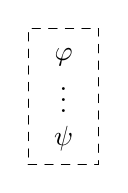
\begin{tikzpicture}
    \node [draw, rectangle, dashed, line cap=round]
    {\begin{tabular}{c} $\varphi$ \\ \vdots \\ $\psi$ \end{tabular}};
  \end{tikzpicture}
  }{\varphi \rightarrow \psi}
  \qquad \infer {
  \begin{tikzpicture}
    \node [draw, rectangle, dashed, line cap=round]
    {\begin{tabular}{c} $\varphi$ \\ \vdots \\ $\bot$ \end{tabular}};
  \end{tikzpicture}
  }{\neg \varphi}
  \qquad \infer {
  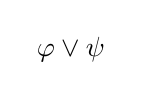
\begin{tikzpicture}
    \node {$\varphi \lor \psi$};
  \end{tikzpicture} \\
  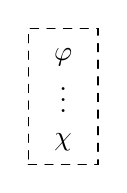
\begin{tikzpicture}
    \node [draw, rectangle, dashed, line cap=round]
    {\begin{tabular}{c} $\varphi$ \\ \vdots \\ $\chi$ \end{tabular}};
  \end{tikzpicture} \\
  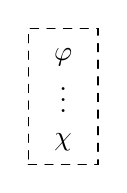
\begin{tikzpicture}
    \node [draw, rectangle, dashed, line cap=round]
    {\begin{tabular}{c} $\varphi$ \\ \vdots \\ $\chi$ \end{tabular}};
  \end{tikzpicture}
  }{\chi}
\]
\end{remark}

\begin{example}
Using the notation from Remark \ref{cl7:rm:box}, we can rewrite the proof for Example
\ref{cl7:ex:contrapositive}:
\[ \infer {
  \begin{tikzpicture}
    \node [draw, rectangle, dashed, line cap=round] {$
    \infer {
      \text{1. } \varphi \rightarrow \psi \\\\
      \begin{tikzpicture}
        \node [draw, rectangle, dashed, line cap=round] {$
        \infer {
          \text{2. } \neg \psi \\\\
          \begin{tikzpicture}
            \node [draw, rectangle, dashed, line cap=round] {
            \begin{tabular}{c}
              3. $\varphi$ \\
              4. $\psi$ ($\rightarrow$-elim, 1, 3) \\
              5. $\bot$ ($\neg$-elim, 2, 4)
            \end{tabular}
            };
          \end{tikzpicture}
        }{\neg \varphi}
        $};
      \end{tikzpicture}
    }{\neg \psi \rightarrow \neg \varphi}
    $};
  \end{tikzpicture}
  }{(\varphi \rightarrow \psi)
    \rightarrow (\neg \psi \rightarrow \neg \varphi)}
\]
\end{example}



\begin{remark}
The system $\nj$ defined is in fact the Intuitionistic Natural 
Deduction system. The following rule, namely the law of excluded
middle, cannot be derived in $\nj$:
\begin{center}
    \AxiomC{}
    \RightLabel{\small (ex)}
    \UnaryInfC{$\Gamma \proofs \varphi \lor  \neg\psi $}
    \DisplayProof.
\end{center}
Assumption of the law of excluded middle is in fact an important
distinction between intuitionistic and classical logic. 
\end{remark}

\begin{definition}[$\nk$]
The system \emph{$\nk$} consists of the same rules as $\nj$ in addition to the law of excluded middle.
\begin{center}
    \AxiomC{}
    \RightLabel{\small (ex)}
    \UnaryInfC{$\Gamma \proofs \varphi \lor  \neg\psi $}
    \DisplayProof.
\end{center}
\end{definition}

\begin{theorem}
The $\nk$ system is sound and complete for propositional logic.
\end{theorem}

\begin{example}
  Show that there exist $a, b \not \in \QN$ such that
  $a ^ b \in \QN$.
\end{example}
\begin{proof}
  Let $a = \sqrt{2} ^ {\sqrt{2}}$ and $b = \sqrt{2}$. We know that
  $\sqrt{2} \not \in \QN$. We do a ``classical''
  case-splitting on $a \in \QN$:
  \begin{itemize}
    \item Case $a \not \in \QN$: We have
    \[ a ^ b
      = \left( \sqrt{2} ^ {\sqrt{2}} \right) ^ {\sqrt{2}}
      = \sqrt{2} ^ 2
      = 2 \in \QN \]
  \item Case $a \in \QN$: We are already done with the proof; let
  $a_1 = b_1 = \sqrt{2}$. We know $a_1, b_1 \not \in \QN$ and,
  by assumption, ${a_1} ^ {b_1} \in \QN$.
  \end{itemize}
  Observe how this classical-style proof utilizes the law of excluded
  middle in the case-splitting: $\sqrt{2} ^ {\sqrt{2}}$ is either in
  $\QN$ or not in $\QN$; there is no \emph{middle}.
\end{proof}



\subsection{Kripke Semantics}

\begin{remark}
Classically, an interpretation $\valfoo\colon P \to \BN$ is defined as a
mapping from a set of propositions to boolean values $\top$ and
$\bot$. For intuitionistic reasoning, we define a new semantics.
\end{remark}

\begin{definition}
  A Kripke model $\kripke$ is defined as a tuple $(W, \krel, w_0,
  \valfoo\colon W \times P \to \BN)$, where $W$ is a set of classical
  worlds, $\krel$ is a pre-order relation on $W$, $w_0$ is the initial
  world, and $\valfoo$ is a function from pairs of world and proposition
  to boolean values such that for any $w, w' \in W$ and any
  $p \in P$, if $w \krel w'$, then $v(w, p) \krel v(w', p)$.
\end{definition}

\begin{remark}
Informally, a Kripke model is an interpretation model for
intuitionistic proof systems. 
\end{remark}

\begin{theorem}
    The following facts hold for any Kripke
model $m$: (i)  $\kripke \models \varphi$ iff $m \proofs_{w_0} \varphi$;
(ii) $\kripke\not \models_w \bot$ for any world $w$; (iii) $\kripke \models_w p$ iff $\valfoo(w, p) = \top$; (iv) $\kripke \models_w \varphi \rightarrow \psi$ iff for any $w'$, if $w \krel w'$ and $\kripke \models_{w'} \varphi$, then $\kripke \models_{w'} \psi$.
\end{theorem}

\begin{remark}
  In $\nj$, whenever you show $\varphi \lor \psi$, you need to show either
$\varphi$, or $\psi$. As previously stated, the law of excluded middle
cannot be derived in $\nj$. To show this, we need to show that there
exists a Kripke model $\kripke$ such that excluded middle is false in a
world $w$ of $\kripke$.  
\end{remark}


\begin{example}
Let us define a Kripke model with only one proposition $p$ and only
two worlds $w_0$ and $w_1$, where $w_0 \krel w_1$, and $p$ is false in
$w_0$ and true in $w_1$.
\begin{center}
  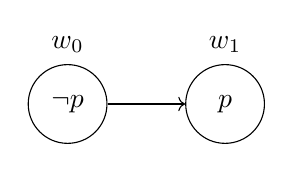
\begin{tikzpicture}
    \node (w0) at (0, 0) [draw, circle,  minimum size=1cm] {$\neg p$};
    \node (w1) at (2, 0) [draw, circle,  minimum size=1cm] {$p$};
    \node at (0, .75) {$w_0$};
    \node at (2, .75) {$w_1$};
    \draw[->] (w0) -- (w1);
  \end{tikzpicture}
\end{center}
Let us examine what formulas are true (or false) in each world. By
definition, $p$ is false in $w_0$. Let us examine the value of
$\neg p$ in $w_0$. We can safely substitute $\neg p$ with $p
\simplies \bot$. By definition, $p \simplies \bot$ holds in
$w_0$ iff for any world $w$, if $w_0 \krel w$ and $p$ is true in $w$,
then $\bot$ is true in $w$. We know $p$ is true in $w_1$. We also
know that $\bot$ is not true in $w_1$, as it is not true in any world.
So, by definition, $p \simplies \bot$ is false in $w_0$. So, both
$p$ and $\neg p$ are false in $w_0$, from which we obtain that $p
\lor \neg p$ is also false in $w_0$.
\end{example}


\subsection{Sequent (Gentzen) Calculus and $\lk$}

\begin{remark}
Judgements in the $\lk$ proof system have the form $\Gamma \proofs
\Delta$, where both $\Gamma$ and $\Delta$ are sets of formulas.
Judgement $\Gamma \proofs \Delta$ should be read as ``the
\emph{conjunction} of the formulas in $\Gamma$ implies the
\emph{disjunction} of the formulas in $\Delta$''. Semantically, for
a classical interpretation $\valfoo$, $\valfoo \models (\Gamma \proofs \Delta)$
if and only if, if all formulas in $\Gamma$ are true under $\valfoo$, then
some formula in $\Delta$ is true under $\valfoo$.
\end{remark}


\begin{definition}
    The Sequent (Gentzen) Calculus is composed of the following rules. 
    (Observe how every non-axiom judgement increases the number of logical
    connectives in the set of formulas.)
    Axioms 
    \begin{center}
      \AxiomC{}
      \RightLabel{\small (ax)}
      \UnaryInfC{$\Gamma, \varphi \proofs \varphi, \Delta$}
      \DisplayProof
      $\quad$
      \AxiomC{}
      \RightLabel{\small $\bot$-elim}
      \UnaryInfC{$\Gamma, \bot \proofs \Delta$}
      \DisplayProof
      $\quad$
      \AxiomC{}
      \RightLabel{\small  $\top$-intro}
      \UnaryInfC{$\Gamma \proofs \top, \Delta$}
      \DisplayProof
    \end{center}
    Conjunction
    \begin{center}
      \AxiomC{$\Gamma, \varphi, \psi \vdash \Delta$}
      \RightLabel{\small($\land$-left)}
      \UnaryInfC{$\Gamma, \varphi \land \psi \vdash \Delta$}
      \DisplayProof
      $\quad$
    \AxiomC{$\Gamma \vdash \varphi, \Delta$}
      \AxiomC{$\Gamma \vdash \psi, \Delta$}
      \RightLabel{\small($\land$-right)}
      \BinaryInfC{$\Gamma \vdash \varphi \land \psi, \Delta$}
      \DisplayProof
      $\quad$
    \end{center}
    Disjunction
    \begin{center}
      \AxiomC{$\Gamma, \varphi \vdash \Delta$}
      \AxiomC{$\Gamma, \psi \vdash \Delta$}
      \RightLabel{\small($\lor$-left)}
      \BinaryInfC{$\Gamma, \varphi \lor \psi \vdash \Delta$}
      \DisplayProof
      $\quad$
      \AxiomC{$\Gamma \vdash \varphi, \psi, \Delta$}
      \RightLabel{\small($\lor$-right)}
      \UnaryInfC{$\Gamma \vdash \varphi \lor \psi, \Delta$}
    \DisplayProof
    \end{center}
    Negation
    \begin{center}
         \AxiomC{$\Gamma, \varphi \vdash \Delta$}
      \RightLabel{$\neg$-right}
      \UnaryInfC{$\Gamma \vdash \neg \varphi, \Delta$}
      \DisplayProof
      $\quad$
       \AxiomC{$\Gamma \vdash \varphi, \Delta$}
      \RightLabel{$\neg$-left}
      \UnaryInfC{$\Gamma, \neg \varphi \vdash \Delta$}
      \DisplayProof
    \end{center}
     Implication
         \begin{center}
  \AxiomC{$\Gamma, \varphi \vdash \psi, \Delta$}
      \RightLabel{$\rightarrow$-right}
      \UnaryInfC{$\Gamma \vdash \varphi \rightarrow \psi, \Delta$}
      \DisplayProof
      $\quad$
      \AxiomC{$\Gamma \vdash \varphi, \Delta$}
      \AxiomC{$\Gamma, \psi \vdash \Delta$}
      \RightLabel{$\rightarrow$-left}
      \BinaryInfC{$\Gamma, \varphi \rightarrow \psi \vdash \Delta$}
      \DisplayProof
    \end{center}
\end{definition}


% \begin{enumerate}
%   \item 
%   \item Conjunction
%   \[ \infer
%     {\Gamma, \varphi, \psi \proofs \Delta}
%     {\Gamma, \varphi \land \psi \proofs \Delta}
%     \qquad\qquad \infer
%     {\Gamma \proofs \varphi, \Delta
%     \\ \Gamma \proofs \psi, \Delta}
%     {\Gamma \proofs \varphi \land \psi, \Delta}
%   \]
%   \item Disjunction
%   \[ \infer
%     {\Gamma, \varphi \proofs \Delta
%     \\ \Gamma, \psi \proofs \Delta}
%     {\Gamma, \varphi \lor \psi \proofs \Delta}
%     \qquad\qquad \infer
%     {\Gamma \proofs \varphi, \psi, \Delta}
%     {\Gamma \proofs \varphi \lor \psi, \Delta}
%   \]
%   \item Negation
%   \[ \infer
%     {\Gamma, \varphi \proofs \Delta}
%     {\Gamma \proofs \neg \varphi, \Delta}
%     \qquad\qquad \infer
%     {\Gamma \proofs \varphi, \Delta}
%     {\Gamma, \neg \varphi \proofs \Delta}
%   \]
%   \item Implication
%   \[ \infer
%     {\Gamma, \varphi \proofs \psi, \Delta}
%     {\Gamma \proofs \varphi \rightarrow \psi, \Delta}
%     \qquad\qquad \infer
%     {\Gamma \proofs \varphi, \Delta
%     \\ \Gamma, \psi \proofs \Delta}
%     {\Gamma, \varphi \rightarrow \psi \proofs \Delta}
%   \]
% \end{enumerate}

\begin{theorem}
    The $\lk$ proof system is sound and complete for propositional logic.
This actually means that excluded middle can be derived in $\lk$.
\end{theorem}


\begin{exercise}
  Prove the following in $\lk$: (i) The law of excluded middle: $ \proofs p \lor \neg p$ and (ii) implication transitivity.
\end{exercise}


\subsection{Decision Procedures}

\begin{remark}
    We now talk about three proof systems for validity: 
    \begin{align*}
            \overset{\text{Hilbert}}{\proofs \varphi} & \quad &  \overset{\text{Natural Deduction}}{\Gamma \proofs \varphi} & \quad &  
            \overset{\text{Grentzen}}{\Gamma \proofs \Delta}
        \end{align*}
\end{remark}
    
\begin{remark}
   We now talk abou three decision procedures (either for validity or for satisfiability)
\end{remark}


\begin{definition}
We define three decision procedures (either for validity or for satisfiability):
(i) Branching (if we don't derive $\bot$ then it is satisfiable)
\begin{center}
    \begin{prooftree}
    \AxiomC{$\Gamma[\top] \; \unsat$ }
    \AxiomC{$\Gamma[\bot]\; \unsat$}
    \BinaryInfC{$\Gamma[p]\; \unsat$}
\end{prooftree}
\end{center}
(ii) Resolution
\begin{center}
    \begin{prooftree}
    \AxiomC{$\Gamma, C_1, C_2, C_1[\bot] \lor C_2[\top]$ $\; \unsat$}
    \UnaryInfC{$\Gamma, C_1[p] , C_2[\neg p]$ $ \; \unsat$}
    \end{prooftree}
\end{center}
(iii) DPLL using unit resolution combined with branching of lower priority ($\ell$ is a literal)
\begin{center}
    \begin{prooftree}
    \AxiomC{$\Gamma, C[\bot]$ $\; \unsat$}
    \UnaryInfC{$\Gamma, \ell, C[\neg \ell]$ $ \; \unsat$}
    \end{prooftree}
\end{center}
\end{definition}

\begin{example}
Consider $p \lor q \lor r ,\; \neg p \lor \neg q \lor \neg r ,\; \neg p \lor q \lor r ,\; \neg q \lor r ,\; q \lor \neg r$
First we branch on $r$.
\begin{align*}
    \text{Case } r=\bot &: & p \lor q ,\; \neg p \lor q ,\; \neg q  &&\overset{Res. \neg q}{\longrightarrow} && p,\;\neg p && \overset{Res. \neg p}{\longrightarrow} &\bot \\
    \text{Case } r=\top &:  & \neg p \lor \neg q &&\overset{q=\top}{\longrightarrow} && \;\neg p && \overset{p=\bot}{\longrightarrow}& \bot
\end{align*}
\end{example}


\begin{definition}[Horn Clauses]
    Horn clause is a clause with at most one positive literal.
\end{definition}


\begin{remark}
    We can view Horn clauses as implications where LHS is a conjunction of positive propositions:
    \begin{align*}
\neg p \lor \neg q 
	&\iff p \land q \simplies \bot \\
\neg p \lor \neg q \lor r 
	&\iff p \land q \simplies r \\
r 
	&\iff \top \simplies r \\
\end{align*}
\end{remark}


\subsection{Metatheorems}

\begin{theorem}
    A countable set $\Gamma$ of formulas is satisfiable iff every finite subset of $\Gamma$ is satisfiable.
\end{theorem}

\begin{theorem}[Craig's interpolation]
    We have $\proofs \varphi \simplies \psi$ iff there exists a third formula $\chi$ (the "interpolant") which only uses
nonlogical symbols (in propositional logic, it is propositions only) that occur in
both $\varphi$ and $\psi$ such that $\proofs \varphi \simplies \chi$ and $\proofs \chi \simplies \psi$.
\end{theorem}

\begin{exercise}
    How hard is it to compute interpolates in propositional logic?
\end{exercise}

\begin{definition}
    The cut rule in $\nk$, $\nj$ (left) and $\lk$ (right) is respectively
    \begin{center}
        \AxiomC{$\Gamma \proofs \varphi$}
        \AxiomC{$\Gamma, \varphi \proofs \psi$}
        \BinaryInfC{$\Gamma \proofs \psi$}
        \DisplayProof
        $\quad$
        \AxiomC{$\Gamma \proofs \varphi, \Delta$}
        \AxiomC{$\Gamma, \varphi \proofs \Delta$}
        \BinaryInfC{$\Gamma \proofs \Delta$}
        \DisplayProof
    \end{center}
\end{definition}

\begin{theorem}[Cut elimination]
\label{cl8:thrm:cut}
    If a judgement can be proved with the cut rule, it can also be proved without the cut rule.
\end{theorem}

\begin{remark}[Theorem \ref{cl8:thrm:cut}]
In fact, it is ``iff''; the other direction is trivial.
Of course, the proof may become longer (introducing a lemma $\varphi$ often helps in practice).
It is a purely syntactic metatheorem. We cannot use deduction to prove it.
\end{remark}

% \subsubsection{Cut elimination}

% Cut rule in NK / NJ:
% $$\inferrule
% {\Gamma\proofs\varphi\qquad\qquad\qquad\Gamma,\varphi\proofs\psi}
% {\Gamma\proofs\psi}
% $$
% Cut rule in LK:
% $$\inferrule
% {\Gamma\proofs\varphi,\Delta\qquad\qquad\qquad\Gamma,\varphi\proofs\Delta}
% {\Gamma\proofs\Delta}
% $$

% If a judgement can be proved with the cut rule, it can also be proved without the cut rule.


\section{First-order logic}


\subsection{Definition}
\begin{remark}
    First-order logic, also called ``predicate logic'', is propositional logic with quantifiers $\forall$ (for all) and $\exists$ (exists).
\end{remark}

\begin{definition}[Signature]
    A Signature defines the non-logical symbols
\begin{itemize}
\item[(i)] finite set of variables $X = \{ x, y, z, \dots \}$
\item[(ii)] finite set of function symbols $F = \{ f, g, h, \dots \}$
\item[(iii)] finite set of predicate symbols $P = \{ p, q, r, \dots \}$
\end{itemize}
Each function symbol has a fixed ``arity'' (number of arguments), which can be zero (arity 0 gives a constant).
Each predicate symbol has also a fixed ``arity'' (number of arguments), which can be zero (arity 0 gives a proposition).
\end{definition}


\begin{definition}[Logical symbols]
The logical symbols consist of:
\begin{itemize}
\item[(i)] connectives ($\bot, \top, \neg, \land, \lor, \simplies$)
\item[(ii)] quantifiers ($\forall, \exists$)
\item[(iii)] finite set of predicate symbols $P = \{ p, q, r, \dots \}$
\end{itemize}
\end{definition}

\begin{remark}
We don't add parentheses to the symbols; we will talk about syntax trees;
only if we want to write them down as strings, we add parentheses (as few as possible).
\end{remark}

\begin{definition}[Syntax]
The syntax of first-order logic is given by the following grammar for terms and formulas repsectively
\begin{align*}
    t &\Coloneqq f_0 \; | \;  f_n(t_1,\dots,t_n) \\
    \varphi &\Coloneqq p_0  \; | \; p_n(t_1,\dots,t_n)  \; | \; \bot  \; | \; \top  \; | \; \neg\varphi  \; | \;\varphi\land\varphi  \; | \; \varphi\lor\varphi  \; | \; \varphi\simplies\varphi  \; | \; \forall x. \varphi  \; | \; \exists x. \varphi
\end{align*}
When we write $\forall x. \varphi$, every occurence of $x$ is bound in $\varphi$.
A variable that is not bound is called free.
A change of bound variables does not change the abstract syntax tree (same in abstract syntax).
\end{definition}


\begin{remark}[Safe substitution]
    If we want to substitute $y^2$ for $x$ in $\forall x\,.\;\, \exists y\,.\;\, y \ge x + 1$, we must first rename $y$ to $z$, i.e., $\forall x\,.\;\, \exists z\,.\;\, z \ge x + 1$, and then substitute, i.e., 
    $\exists z\,.\;\, z \ge y^2 + 1$.
\end{remark}




\begin{definition}[Interpretation]
    Interpretation $\interp$ in first-order structure: 
    \begin{itemize}
        \item[(i)] Domain $D_{\interp}$
        \item[(ii)] for each $n$-ary function symbol $f \in F$, $\eval{f}_{\interp}: D_{\interp}^n \to D_{\interp}$
         \item[(iii)]  for each $n$-ary predicate symbol $p \in P$, $\eval{p}_{\interp}: D_{\interp}^n \to B = \{true,false\}$
        \item[(iv)]  "context" (environment) for each (free) variable $x \in X$, $\eval{x}_{\interp} \in D_{\interp}$
    \end{itemize}
    Formula $\varphi$ is closed if it has no free variables.
\end{definition}


\begin{definition}[Semantics]
Given an interpretation $\interp$, a term $t$ and a formula $\varphi$ have the following meaning: 
\begin{align*}
     \eval{t}_{\interp} &\coloneqq \begin{cases}
         \eval{x}_{\interp} & t=x  \\
         \eval{f}_{\interp}([ \eval{t_1}_{\interp},  \eval{t_2}_{\interp}, \dots,  \eval{t_n}_{\interp}) & t=f(t_1, \dots, t_n)
    \end{cases} \\
     [\varphi]_{\interp} &\coloneqq \begin{cases}
        \eval{x}_{\interp} & t=x  \\
        \eval{p}_{\interp}(\eval{t_1}_{\interp}, \eval{t_2}_{\interp}, \dots, \eval{t_n}_{\interp}) & \varphi = p(t_1, \dots, t_n)
    \end{cases}\\
     \eval{\varphi_1 \simplies \varphi_2}_{\interp} &\coloneqq \true \; \textit{ iff } \; \eval{\varphi_1}_{\interp} = \false \textit{ or } \eval{\varphi_2}_{\interp} = \true \\
     \eval{\forall x. \varphi}_{\interp} &\coloneqq \true \; \textit{ iff for all } \;  d \in D_{\interp}, \eval{\varphi}_{I[x \to d]}=\true \\ 
     \eval{\exists x. \varphi}_{\interp} &\coloneqq \true \; \textit{ iff for some } \; d \in D_{\interp}, \eval{\varphi}_{I[x \to d]}=\true
\end{align*}
\end{definition}

\begin{definition}[Satisfiable and Valid]
    Let $\varphi$ be a first-order formula. The formula $\varphi$ is: 
     (i)\emph{satisfiable} iff it is true for \emph{some} interpretation $\interp$, i.e., $\exists \interp . \models \varphi$.
    (ii) \emph{valid} iff it is true for \emph{all} interpretations $\interp$, i.e., $\forall \interp . \models \varphi$.
\end{definition}


\begin{definition}[Post Correspondence Problem]
    PCP (Post Correspondence Problem): Given a finite set $S$ of dominoes $\frac{s}{t}$ where $s,t \in \{0,1\}^*$. Is there a finite sequence $\frac{s_1}{t_1}, \dots \frac{s_n}{t_n}$ of (possibly repeating) dominoes from $S$ such that the 
$$s_1 \cdot s_2 \cdot \dots \cdot s_n = t_1 \cdot t_2 \dots \cdot t_n$$
\end{definition}

\begin{theorem}
    The PCP problem is undecidable.
\end{theorem}


\begin{theorem}[Compactness] 
The set of formulas $\Gamma$ is satisfiable iff every finite subset of $\Gamma$ is satisfiable.
\end{theorem}


\begin{theorem}[Lowenheim-Skolem] 
If a set $\Gamma$ of formulas is satisfiable then $\Gamma$ is satisfiable by an interpretation with countable domain. 
\end{theorem}


\begin{theorem}[Undecidability]
    Both the validity and satisfiability problems for FOL are undecidable.
\end{theorem}
\begin{proof}
   Let $F = \{e,f_0, f_1\}$ where $e$ is 0-ary and $f_0,f_1$ are unary. With those functions we can encode the string $011$ as $f_1(f_1(f_0(e)))$.  
    Let $P = \{p\}$ where $p$ is a binary predicate. Intuitively, the domino $\frac{s}{t}$ is represented by $p(s,t)$. 
    Given an instance $R\coloneqq \{r_1, \dots, r_k\}$ of PCP we define the formulas
    \begin{align*}
        \varphi_1 &\coloneqq \bigwedge_{1 \leq i \leq k} P(s_{\interp}(e), t_{\interp}(e)) \\
        \varphi_2 &\coloneqq \forall v,w. (p(v,w) \simplies \bigwedge_{1 \leq i \leq k} p(s_{\interp}(v), t_{\interp}(w))) \\ 
        \varphi_3 &\coloneqq \exists z. p(z,z)
    \end{align*}
    It remains to be shown that the formula $\varphi_R = (\varphi_1 \land \varphi_2) \simplies \varphi_3$ is valid iff the answer to $R$ is yes.
\end{proof}

\begin{exercise}
	 Use PCP to show satisfiability of FOL is undecidable. 
\end{exercise}

\subsection{Three Sound and Complete Proof Systems}


\begin{definition}[Hilbert]
We extend the Hilbert system $\hilbert$ by adding the following axioms
\begin{align*}
    (1) \quad & \quad (\forall x. \varphi) \simplies \varphi[x\coloneqq t] \\
    (2) \quad & \quad \forall x. (\varphi \simplies \psi) \simplies (\forall x. \varphi) \simplies (\forall x. \psi) \\ 
    (3) \quad & \quad \varphi \simplies \forall x. \varphi \quad \text{provided $x$ is not free in $\varphi$}
\end{align*}
We denote the safe replacement of every free variable $x$ in $\varphi$ by $t$ as $\varphi[x\coloneqq t]$
\end{definition}



\begin{definition}[Genzen]
We extend the Genzen system $\lk$ by adding the following rules for the $\forall$-quantifier
\begin{center}
    \AxiomC{$\Gamma, \varphi[x\coloneqq t] \proofs \Delta$}
    \RightLabel{\small ($\forall$-elim)}
    \UnaryInfC{$\Gamma, \forall x. \varphi \proofs \Gamma$}
    \DisplayProof 
    $\quad$
    \AxiomC{$\Gamma \proofs \Delta, \varphi[x\coloneqq y]$}
    \RightLabel{\small ($\forall$-intro)}
    \UnaryInfC{$\Gamma \proofs \Delta, \forall x. \varphi$}
    \DisplayProof 
\end{center}
and for the $\exists$-quantifier
\begin{center}
    \AxiomC{$\Gamma, \varphi[x\coloneqq y]$}
    \RightLabel{\small ($\exists$-elim)}
    \UnaryInfC{$\Gamma, \exists x. \varphi \proofs \Delta$}
    \DisplayProof 
    $\quad$
        \AxiomC{$\Gamma \proofs \Delta, \varphi[x\coloneqq t]$}
    \RightLabel{\small ($\exists$-intro)}
    \UnaryInfC{$\Gamma \proofs \Delta, \exists x. \varphi$}
    \DisplayProof 
\end{center}
where $y$ is a new (fresh) variable.
\end{definition}


\begin{definition}[Natural Deduction]
    We extend the Natural Deduction system $\nk$ (and $\nj$) by adding the following rules for the $\forall$-quantifier
\begin{center}
    \AxiomC{$\forall x. \varphi$}
    \RightLabel{\small ($\forall$-elim)}
    \UnaryInfC{$\varphi[x\coloneqq t]$}
    \DisplayProof 
    $\quad$
    \AxiomC{$\varphi[x\coloneqq y]$}
    \RightLabel{\small ($\forall$-intro)}
    \UnaryInfC{$\forall x. \varphi$}
    \DisplayProof 
\end{center}
and for the $\exists$-quantifier
\begin{center}
    \AxiomC{$\exists x . \varphi$}
            \AxiomC{$\varphi[x\coloneqq y]$}
            \noLine
        \UnaryInfC{$\vdots$}
        \noLine
    \UnaryInfC{$\psi$}
    \RightLabel{\small ($\exists$-elim)}
    \BinaryInfC{$\psi$}
    \DisplayProof 
    $\quad$
        \AxiomC{$\varphi[x\coloneqq t]$}
    \RightLabel{\small ($\exists$-intro)}
    \UnaryInfC{$\exists x. \varphi$}
    \DisplayProof 
\end{center}
where $y$ is a new (fresh) variable.
\end{definition}



\begin{exercise} 
Prove de Morgan, i.e., $ \forall x. \varphi \Leftrightarrow \neg \exists x. \neg \varphi$, for quantifiers in all three systems.
\end{exercise}

\subsection{First Order Resolution: Classical Automated Theorem Proving} 



\begin{definition}[First Order Resolution]
    To proof $\models \varphi $ for a closed $\varphi $:
\begin{enumerate}
    \item Negate. Show $\neg \varphi $ is unsat.
    \item Bring $\neg \varphi $ into "prenex" form (see Remark \ref{cl10:rem:prenex}).
    \item Bring $\gamma$ into CNF.
    \item "Skolemization" gets rid of $\exists$ (see Remark \ref{cl10:rem:skolem}). 
    \item Drop $\forall$.
    \item See Theorem \ref{cl10:thrm:unifier}
\end{enumerate}
\end{definition}


\begin{remark}[Prenex]
\label{cl10:rem:prenex}
A formula is in prenex normal all quantifiers are in the front, e.g., $\exists x. \varphi (x) \land \gamma \siff \exists x (\varphi (x) \land \gamma)$.
\end{remark}


\begin{remark}[Skolemization]
\label{cl10:rem:skolem}
    Consider that  while for $\exists x.\varphi (x)$ is sat iff $\varphi (\hat{x})$ is sat, we have that $\forall y \exists x \varphi (x)$  is sat iff $\varphi (f(y))$ is sat where $f(y)$ is a new function symbol. Thus,for each $\exists x$ within the scope of a universally quantified variables $y_1, \cdots,y_n$, drop $\exists x$ and replace each bound occurrence of x by $f(y_1,\cdots,y_n)$ where f is a new n-ary function symbol. E.g. 
        \begin{align*}
            \forall x, \exists y \forall z_1,z_2 \exists y . \varphi  (x,y,z_1,z_2, u) \rightarrow \forall x \forall z_1, z_2. \varphi  (x, f(x), z_1, z_2, g(x, z_1,z_2)).
        \end{align*}
\end{remark}

\begin{theorem}[Unifier]
    \label{cl10:thrm:unifier}
    For an interpretation $\interp$, clauses $C_1$ and $C_2$, and literals $\ell $ and $\ell '$. If $\interp \models C_1[\ell]$ and $\interp \models C_2[\neg \ell']$ and $\ell , \ell'$ are "unifiable" (i.e, there is a substitution, which is a function from variables to terms, that when applied to $\ell $ and $\ell '$, makes them equal), then $\interp \models X_1\theta [\bot] \lor C_2\theta [\bot]$ where $\theta$ is the most general unifier of $\ell $ and $\ell '$.
\end{theorem}


\begin{example}
        For example for a variable $x$ and a constant $S$, we have that $m(x)$ and $\neg m(S)$ are unifiable by replacing $x $ by $s$. The purpose is to make literals the same.
\end{example}

\subsection{First order theories} 


\begin{remark}
    Theories defined by (i) signature (set of functions + predicate symbols) and (ii) either by a r.e. set of closed formulas called axioms $A$ (set of all $A$-valid closed formulas) or by a specific "intended" interpretation $\interp$ (true formulas in $\interp$).
\end{remark}

\begin{definition}
    A theory $T$ is a r.e. set of closed formulas (there are no free variables) that are closed under $\models$, i.e 
     $T \models \varphi $  iff $\forall \interp ((\forall \psi \in T.  \interp \models \psi) \simplies  \interp \models \varphi )$. 
\end{definition}
Formally, 

\begin{definition}
    We say that 
\begin{itemize}
    \item $\varphi $ is $T$-valid iff $T \models \varphi $
    \item $\varphi $ is $T$-satisfiable iff $\exists  \interp.  \interp$ T-model $\varphi $.
    \item $ \interp$ is a $T$-model iff $\forall \psi \in T.  \interp \models \psi$.
    \item $\varphi , \psi$ are $T$-equivalent iff $\varphi ,\psi$ have truth value in all $T$-models.
\end{itemize}
\end{definition}

\begin{remark}
    \label{cl10:rem:theory}
    Therefore, $T$ is either (i) the set of all $A$-valid closed formulas or (ii) $T$ is the set of all formulas true in $\interp$.
\end{remark}


\begin{definition}
    The theory $T$ is: 
    \begin{itemize}
        \item   \emph{consistent} iff $\exists \interp. \forall \psi \in T$, $\interp\models \psi$ (always the case for (ii) in Remark 
        \ref{cl10:rem:theory}); 
        \item \emph{complete} iff for all closed formulas $\psi$ of the signature, either $T \models \psi$ or $T \models \neg \psi$ (always the case for (ii) in Remark \ref{cl10:rem:theory});
        \item  $T$ is \emph{decidable} iff the problem "given $\psi$, is $T \models \psi$" is decidable.
    \end{itemize}
\end{definition}


\begin{remark}
    Common theories are the theory of:
    (i)  propositional logic with quantifiers (QBF);
    (ii) equality with uninterpreted functions and predicates;
    (iii) the integers, either Peano- or Pressburger arithmetic;
    (iv) the reals over real closed fields; 
    (v) the rational numbers with linear arithmatic;
    (vi) lists and arrays.
\end{remark}



\begin{definition}[$T_{EQ}$]
\label{cl11:def:theory-equality}
The theory of equality and uninterpreted function + predicate symbols $T_{EQ}$ has as signature $(=)$ and is composed of the following axioms 
\begin{itemize}
    \item[(i)] equivalence axiom: $=$ is equivalence
    \item[(ii)] congruence axiom: for every function symbol $f$, $\forall x_1, \cdots, x_n, y_1, \cdots, y_n$,
    \begin{align*}
        x_1 = y_1 \land \cdots \land x_n=y_n \Rightarrow f(x_1, \cdots, x_n) = f(y_1, \cdots, y_n)
    \end{align*}
    and for every predicate $p$, $\forall x_1, \cdots, x_n, y_1, \cdots, y_n$, 
    \begin{align*}
         x_1 = y_1 \land \cdots \land x_n=y_n \Rightarrow p(x_1, \cdots, x_n) = p(y_1, \cdots, y_n).
    \end{align*}
\end{itemize}
\end{definition}

% Quantifier free fragment: given quantifier free formula $\phi$, is $\phi$ $T$-satisfiable? 
\begin{theorem}
Satisfiability of quantifier free $T_{EQ}$ is NP-complete. 
Satisfiability of quantifier free conjunction of $T_{EQ}$ with congruence closure is $O(n \log n)$. 
\end{theorem}

\begin{remark}[Congruence Closure] 
First replace predicate by function symbols, i.e., replace $p(t_1, \cdots, t_n)$ by $ f_p(t_1, \cdots, t_n) = T $.
Second the conjunction $\phi := (\land _i s_i = t_i) \land (\land_j s_j \neq t_j)$ is satisfiable iff there exists a congruence relation on terms (i.e., a relation satisfying (i) and (ii) in Definition \ref{cl11:def:theory-equality}, and for all $i$, $s_i=t_i$, and for all $j$, $s_j \neq t_j$) 
\end{remark}
    





\begin{example}[Congruence Closure] 
To show that $\phi := f^3(a) = a \land f^5(a) = a \land f(a) \neq a$ is unsatisfiable with congruence closure we follow the steps
\begin{align*}
    &\{a\}, \{f(a)\}, \cdots, \{f^5(a)\} \\
&\{a, f^3(a)\}, \{f(a), f^4(a)\}, \{f^2(a), f^5(a)\} \\
&\{\mathbf{a}, f^2(a), f^3(a), f^5(a), \mathbf{f(a)}, f^4(a)\}
\end{align*}
\end{example}


\begin{exercise}
    Given union find, write congruence closure (subquadratic)? 
\end{exercise}



\begin{definition}[$T_{GR}$]
  The theory of groups ($T_{GR}$) has the signature $(=, \cdot, i, -)$ and consists of the following axioms.
\begin{align*}
\text{(i)} \quad & \forall x,y,z, \quad (x \cdot y) \cdot z = x \cdot (y \cdot z) \\
\text{(ii)} \quad & \forall x, \quad x \cdot i = x \\
\text{(iii)} \quad & \forall x, \quad x \cdot (-x) = i \\
\text{(iv)} \quad & \forall x,y, \quad x \cdot y = y \cdot x \quad \text{(Abelian)}  . 
\end{align*}
\end{definition}

\begin{theorem}
    The theory $T_{GR}$ is incomplete and undecidable. 
\end{theorem}



\begin{exercise}
    Analyze the quantifier-free $T_{GP}$. Is it undecidable and/or incomplete?
\end{exercise}




\begin{definition}[$T_{\NN}$]
\label{cl11:def:theory-nn}
 Theory of the natural numbers ($T_{\NN}$) has the signature $(=, 0, 1, +, \cdot)$. There are two different set of axioms, i.e., the Peano arithmetic (Definition \ref{cl11:def:peano}) and Presburger arithmetic (Remark \ref{cl11:rem:pres}).
\end{definition}





\begin{definition}[$T_{PE}$]
\label{cl11:def:peano}
Given the signature in Definition \ref{cl11:def:theory-nn}, the theory of Peano arithmetic ($T_{PE}$) is defined w.r.t.\ the following axioms. 
 \begin{align*}
\text{(i)} \quad &\forall x, \quad Sx \neq 0 \\
\text{(ii)} \quad &\forall x,y, \quad Sx = Sy \simplies x=y \\
\text{(iii)} \quad&\phi(0) \land \forall x (\phi(x) \simplies \phi(x+1)) \simplies \forall x, \phi(x) \\
\text{(iv)} \quad&\forall x, \quad x + 0 = x \\
\text{(v)} \quad&\forall x,y, \quad x + Sy = S (x+y) \\
\text{(vi)} \quad&\forall x, \quad x \cdot 0 = 0 \\
\text{(vii)} \quad&\forall x,y, \quad x \cdot Sy = xy + x .
 \end{align*}
\end{definition}

\begin{theorem}
The theory $T_{PE}$ is incomplete and undecidable,  
including its quantifier-free fragment (see Goedel).
\end{theorem}

\begin{remark}[$T_{PR}$]
\label{cl11:rem:pres}
   The theory of Presburger arithmetic is defined over the same signature as in Definition \ref{cl11:def:theory-nn} is an alternative axiomatisation of the natural numbers. The axioms are omitted.
   No quantifier elimination (QE) is possible in this theory.
   Where QE means that for every formula $\forall x$, $\phi (x, y_1, \cdots, y_n)$, there exists a $T$-equivalent $\psi (y_1, \cdots, y_n)$. 
\end{remark}

\begin{theorem}
    The theory $T_{PR}$ is complete and decidable in $3\mathrm{EXP}$. The quantifier free fragment is in $\mathrm{NP}$.
\end{theorem}

\begin{exercise}
    Give a $T_{PR}$ formula that has no quantifier-free equivalent. 
\end{exercise}

\begin{definition}[$T_{\RN}$]
      The theory of the reals ($T_{\RN}$) has the signature $(=, 0, 1, +, -, \cdot, \leq)$ and consists of the following axioms.
      \begin{align*}
          \text{G-(i)} \quad&  (+,0) ;&&\text{Abelian group} \\
          \text{R-(i)}\quad& (xy)z=x(yz),\; && \text{Ring} \\
        \text{R-(ii)}\quad&   x \cdot 1 = 1 \cdot x = x, &&\; \\
          \text{R-(iii)}\quad&  (x+y)z = xz + yz,&& \\
          \text{R-(iv)}\quad &  x(y+z) = xy + xz; &&\\
          \text{F-(i)}\quad& xy=yx,\; && \text{Field} \\
        \text{F-(ii)}\quad&  0 \neq 1,&& \\
        \text{F-(iii)}\quad&  x \neq 0 \simplies \exists y . xy=1;&& \\
        \text{O-(i)}\quad& x \leq y \land y \leq x \simplies x=y && \text{Order} \\
        \text{O-(ii)}\quad& x \leq y \land y \leq z \simplies x \leq z,&& \\
         \text{O-(iii)}\quad& x \leq y \lor y \leq x;&& \\
        \text{(i)}\quad& \forall x\exists y. \; x = yy \lor -x = yy &&  \\
        \text{(ii)}\quad& \forall x_1, \cdots,x_n \exists y. \; y^n + x_1y^{n-1} + \cdots + x_{n-1}y + x_n = 0 && \text{(odd $n$)} \\
      \end{align*}      
\end{definition}


\begin{theorem}
    The theory $T_{\RN}$ is complete and decidable in $2\mathrm{EXP}$ using cylindrical algebraic decomposition for QE.
\end{theorem}


\begin{definition}[$T_{\mathrm{LI}}$]
    The theory of linear arithmetic ($T_{\mathrm{LI}}$) has the signature $(=, 0, 1, +, -,\leq)$ and consists of the following axioms.
      \begin{align*}
    \text{(i)}\quad& \leq \quad \text{anti-symmetric, transitive, total} \\
    \text{(ii)}\quad& + \quad \text{associative, commutable, identity $0$, inverse $-$} \\
    \text{(iii)}\quad&\forall x\, y\, z. \; x\geq y \simplies x+z \geq y+z \\
    \text{(iv)}\quad&\forall x . \; nx=0 \simplies x=0 \quad \text{for all $n$}\\
    \text{(v)}\quad&\forall x\, \exists y. \; x=ny \quad \text{for all $n>0$} \\
  \end{align*}      
\end{definition}

\begin{theorem}
    The theory $T_{\mathrm{LI}}$ is complete and decidable in  $2\mathrm{EXP}$ using Fourier-Motzkin for QE.
\end{theorem}


\begin{example}
Starting with the set of equations 
\begin{align*}
    \left\lbrace x_1 - x_2 \leq 0 , \;
    x_1 - x_3 \leq 0 ,\; 
-x_1 + x_2 + 2x_3 \leq 0 ,\;
-x_3 \leq 1\right\rbrace . 
\end{align*}
we first eliminate $x_1$ obtaining 
\begin{align*}
   \left\lbrace x_1 \leq x_2 ,\; x_1 \leq x_2 ,\;  x_1 \geq x_2 + 2 x_3 \right\rbrace .
\end{align*}
Next we get 
\begin{align*}
   \left\lbrace 
      2x_3\leq 0 ,\; 
    x_2 + x_3 \leq 0,\; 
    -x_3 \leq 1
   \right\rbrace .
\end{align*}
Eliminating $x_2$ we obtain
\begin{align*}
   \left\lbrace 
      x2\leq -x_3 ,\; 
     x_3 \leq 0,\; 
    -x_3 \leq 1
   \right\rbrace.
\end{align*}
Finally eliminating $x_3$ to obtain $\top$. 
\end{example}

\begin{remark}
    Linear inequalities over $\QN$ are $\mathrm{NP}$-complete, e.g., integer linear programming. 
\end{remark}

\begin{definition}[$T_{\mathrm{List}}$]
    The theory of list ($T_{\mathrm{List}}$), or recursive data structures, has the signature $(=, \tatom, \tcar, \tcdr, \tcons)$ where: $\tatom$ is a unary predicate, 
    $\tcar$ and $\tcdr$ are unary functions, and $\tcons$ is a binary function.
    The theory consists of the following axioms
    \begin{align*}
        (i) \quad &\forall x, y. \, \tcar(\tcons(x,y,)) = x \\
        (ii) \quad &\forall x, y. \, \tcdr(\tcons(x,y,)) = y \\
        (iii) \quad &\forall x, y. \, \neg\tatom(\tcons(x,y,))  \\
        (iv) \quad &\forall x. \, \neg\tatom(x)  \simplies \tcons(\tcar(x), \tcdr(x))=x \\
        (v) \quad &\forall x. \, \tatom(x)  \simplies \varphi[x] \land \forall x,y .(\tatom(x) \land \underbrace{\varphi[y]}_{\text{IH}} \simplies \varphi[\tcons(x,y)]) \simplies \forall x. \varphi[x] 
    \end{align*}
    Where (i),(ii) are destructor axioms, (v) is the constructor axiom, and (vi) is the induction scheme. 
\end{definition}

\begin{theorem}
    The theory $T_{\mathrm{List}}$ is undecidable (decidable if quantifier-free), consistent and incomplete.
\end{theorem}
\begin{example}
    The list $(1\; 2 \; 3)$ can be represented as $(\tcons(1, \tcons(2,3)))$
\end{example}


\begin{definition}[$T_{\mathrm{Array}}$]
    The theory of arrays ($T_{\mathrm{Array}}$) has the signature $(=, \tread, \twrite, \tcdr, \tcons)$ where: $\tread$ is a binary function, e.g., $\tread(a,i)$ reads array $a$ at index $i$ and returns a value; $\twrite(a,i,x)$ writes the value $x$ at position $i$ in array $a$. 
    The theory consists of the following axioms
    \begin{align*}
        (i) \quad & \forall a\forall i,j \forall x . \; i=j \simplies \tread(\twrite(a, i, x),j) = x \\
        (ii) \quad & \forall a\forall i,j \forall x . \; i\ne j \simplies \tread(\twrite(a, i, x),j) = \tread(a, j) \\        
    \end{align*}
    Where (i),(ii) are destructor axioms, (vi) is the constructor axiom, and (v) is the induction scheme. 
\end{definition}


\begin{theorem}
    The theory $T_{\mathrm{List}}$ is undecidable (decidable if quantifier-free), consistent and incomplete.
\end{theorem}


\begin{remark}[QBF]
    Quantified boolean formulas have an empty signature and no axioms. They are in $\mathrm{PSPACE}$, i.e., decidable, (quantifier-free $\mathrm{NP}$), and complete.
\end{remark}

\begin{remark}[Combination of theories]
    The Nelson-Oppen Algorithm can be used to combine theories. 
    If the satisfiability of quantifier-free formulas of $T_1$ and $T_2$ are decidable, then the Nelson-Oppen Algorithm decides the satisfiability of quantifier-free formulas in the combined theory $T_1 \oplus T_2$ (the axioms of $T_1 \oplus T_2$ is the union of the respective axioms).
    The condition is that $T_1$ and $T_2$ are stably infinite and contain $=$. 
\end{remark}

\begin{definition}
    The theory $T$ is stable infinite if for all quantifier-free $\varphi$, if $\varphi $is satisfiable then there exists a $T$-interpretation $\interp$ with inf. domain s.t. $\interp\models \varphi$.
\end{definition}


\begin{remark}[Nelson-Oppen Algorithm]
    The Nelson-Oppen Algorithm for the combined theory $T_1 \oplus T_2$ of $T_1$ and $T_2$ has two steps:
    \begin{itemize}
        \item \emph{Step 1: Purification} Given a formula $\varphi$ in $T_1 \oplus T_2$ construct $\varphi_1$ in $T_1$  and $\varphi_2$ in $T_2$ s.t. $\varphi$ is satisfiable iff $\varphi_1\land \varphi_2$ is satisfiable.

        \item \emph{Step 2: Equality propagation:} $\varphi_1\land \varphi_2$ is satisfiable iff there exists an equivalence relation $\sim$ on the variables with characteristic formula $\psi_{\sim}$ s.t. $\varphi_1\land \psi_{\sim}$ and $\varphi_2\land \psi_{\sim}$ satisfiable
        \begin{align*}
            \psi_{\sim}\coloneqq \bigwedge_{x \sim y} x=y \land \bigwedge_{x\not\sim y} x\neq y 
        \end{align*}
    \end{itemize}
\end{remark}


\begin{example}
    Consider the combined theory of Presburger arithmetic and uninterpreted functions.
    Then the purification step of $\varphi$ into $\varphi_1$ and $\varphi_2$ results in the following
    \begin{align*}
        \varphi&\coloneqq (1\leq x\leq 2\land f(1)\neq f(x) \land f(2)\neq f(x)) \\
        \varphi_1&\coloneqq (1\leq x\leq 2\land y_1=1 \land y_2=2) \\
         \varphi_2&\coloneqq ( f(1)\neq f(x) \land f(2)\neq f(x)) \\
    \end{align*}
    We then have the equivalence relation $\sim\coloneqq \{\{x,y_1\}, \{y_2\}\}$ and 
    \begin{align*}
        \psi_{\sim}\coloneqq (x=y_1\land x\neq y_2 \land y_1\neq y_2)
    \end{align*}
    for the equality propagation step.
\end{example}





\section{Lambda Calculus}

\begin{remark}
    The term $\lambda x.t$ denotes the function that maps x to $t(x)$, e.g., $(\lambda y. \lambda x. x^2 \cdot y)(2) = \lambda x.2x^2$.
\end{remark}

\begin{definition}[Lambda Calculus: Syntax]
    The syntax of Lambda calculus is given be the following grammar
    \begin{align*}
        t\Coloneqq x \; \mid \; \lambda x.t \; \mid \;  t_1 \, t_2
    \end{align*}
    where $x$ is a variable, $\lambda x.t $ is an abstraction, and $ t_1 \, t_2$ is an application. Application is left-associated, i.e., $(t_1 \, t_2)\, t_3 = t_1 \, t_2 \, t_3$, and binds stronger than abstraction, i.e., $\lambda x.(t_1 \, t_2)=\lambda x. t_1 \, t_2$ (not to be confused with $(\lambda x.t_1) \, t_2$).
\end{definition}


\begin{definition}[Lambda Calculus: Operational semantics]
    We have the axiom $\beta$-reduction, i.e.,
    \begin{prooftree}
        \AxiomC{}
        \UnaryInfC{$(\lambda x.t)s \to_{\beta} t[x\mapsto s]$}
    \end{prooftree}
    where $t[x\mapsto s]$ indicates safe substitution, and the proof rules congruence 
    \begin{center}
        \AxiomC{$t\to_{\beta} t' $}
        \UnaryInfC{$\lambda x.t  \to_{\beta} \lambda x.t'$}
        \DisplayProof
        \quad
        \AxiomC{$t\to_{\beta} t' $}
        \UnaryInfC{$t\, s  \to_{\beta} t'\, s$}
        \DisplayProof
        \quad 
        \AxiomC{$t\to_{\beta} t' $}
        \UnaryInfC{$s\,t \to_{\beta}s \, t'$}
        \DisplayProof
    \end{center}
    
\end{definition}


\begin{remark}[Nondeterministic]
    Lambda calculus is nondeterministic, e.g.,
     \begin{center}
     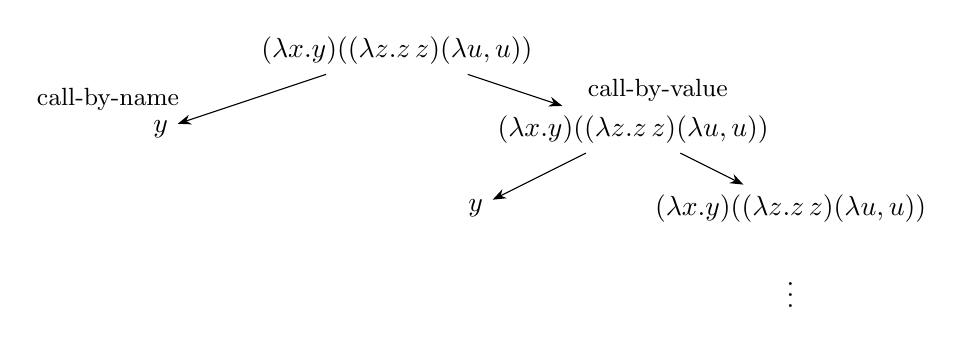
\begin{tikzpicture}[->, >=Stealth]


    \node (0) at (0, 0) {$(\lambda x. y)((\lambda z. z\, z)(\lambda u, u))$};
    \node (1) at (-3, -1) {$y$};
    \node (2) at (3, -1) {$(\lambda x. y)((\lambda z. z\, z)(\lambda u, u))$};
    \node (3) at (1, -2) {$y$};
    \node (4) at (5, -2) {$(\lambda x. y)((\lambda z. z\, z)(\lambda u, u))$};
    \node (5) at (5, -3) {$\vdots$};

    \draw (0) -- (1) node[midway, left=0.8cm] {\small call-by-name};
    \draw (0) -- (2) node[midway, right=0.8cm] {\small call-by-value};
    \draw (2) -- (3) node[midway, right] {};
    \draw (2) -- (4) node[midway, right] {};
% % Edges
% \draw (0) -- (A) node[midway, below] {\small $\true$};
% \draw (C) -- (1) node[midway, above] {\small$x=m\cdot n$};
% \draw (A) -- (B) node[midway, left] {\small$x=0$};
% \draw (B) -- (C) node[midway, left] {\small$x=0\land y=0$};
% \draw (C) -- (D) node[midway, right=0.5cm] {\small$x=m\cdot y \land y<n$};
% \draw (D) -- (E) node[midway, right=0.5cm] {\small$x=m\cdot (y+1) \land y<n$};
% \draw (E) -- (C) node[midway, left] {\small$x=m\cdot (y) \land y\leq n$};

\end{tikzpicture}
 \end{center}
\end{remark}


\begin{theorem}[Confluence]
    For all $t, t_1, t_2$ if $t \to_{\beta}^* t_1$ and $t \to_{\beta}^* t_2$ then there exists an $s$ such that $t_1 \to_{\beta}^* s$ and $t_2 \to_{\beta}^* s$, where $ \to_{\beta}^*$ is the reflexive, transitive closure of $\to_{\beta}$.
\end{theorem}

\begin{remark}
    The confluence theorem is also known as the Church Rosser theorem or the Diamond theorem.
         \begin{center}
     \begin{tikzpicture}[->, >=Stealth]


    \node (0) at (0, 0) {$t$};
    \node (1) at (-1, -1) {$t_1$};
    \node (2) at (1, -1) {$t_2$};
    \node (3) at (0,-2) {$s$};
    
  

    \draw (0) -- (1) node[midway, left=0.8cm] {};
    \draw (0) -- (2) node[midway, right=0.8cm] {};
    \draw (1) -- (3) node[midway, right] {};
    \draw (2) -- (3) node[midway, right] {};
% % Edges
% \draw (0) -- (A) node[midway, below] {\small $\true$};
% \draw (C) -- (1) node[midway, above] {\small$x=m\cdot n$};
% \draw (A) -- (B) node[midway, left] {\small$x=0$};
% \draw (B) -- (C) node[midway, left] {\small$x=0\land y=0$};
% \draw (C) -- (D) node[midway, right=0.5cm] {\small$x=m\cdot y \land y<n$};
% \draw (D) -- (E) node[midway, right=0.5cm] {\small$x=m\cdot (y+1) \land y<n$};
% \draw (E) -- (C) node[midway, left] {\small$x=m\cdot (y) \land y\leq n$};

\end{tikzpicture}
 \end{center}
\end{remark}

\begin{definition}
    The term $t$ is irreducible (in ``normal form''), if for all $t'$, $t\not\to_{\beta} t'$. 
\end{definition}

\begin{corollary}
    For all $t, t_1, t_2$ if $t \to_{\beta}^* t_1$ and $t \to_{\beta}^* t_2$ and
    if $t_1$ and $t_2$ are in normal form, then $t_1=t_2$.
\end{corollary}

\begin{remark}
    The term $t$ can only be irreducible, if it has the form $\lambda x.t'$ with $t'$ being irreducible, or if it has the form $t= t_1 \dots t_n$ and $t_1, \dots t_n$ are irreducible. If you start from a closed term then the only normal forms are $\lambda x t$ terms. 
\end{remark}

\begin{remark}
    There are infinite computations of the term $(\lambda x. x\, x)(\lambda x. x\, x)$.
\end{remark}

\begin{definition}
    A term $t$ is weakly normalizing, if some computation from $t$ terminates. It is strongly normalizing if all computations from $t$ terminate
\end{definition}

\begin{theorem}[Church]
    The problem whether $t$ is (weakly) normalizing is undecidable, i.e., the halting problem for $\lambda$-calculus.
\end{theorem}
\subsection{Encoding $\mathbb{N}$ in $\lambda$ (Church numerals)}



\begin{definition}[$\BN$]
The booleans $\BN$ are defined in $\lambda$-calculus as
\begin{align*}
    \top \coloneqq \lambda x \lambda y.x = \lambda x y. x  \quad \text{and} \quad  \bot \coloneqq \lambda x \lambda y.y = \lambda x y. y.
\end{align*}
Moreover, if is defined as $\lif \coloneqq \lambda b x y. bxy$.
    
\end{definition}


\begin{example}
The expression $\lif \top  s  t$ reduces as follows.
\begin{align*}
\lif \top  s  t  = \quad  &(\lambda bxy.bxy)(\lambda xy.x)st \to (\lambda xy.(\lambda xy.x)xy)st \to (\lambda y.(\lambda xy.x)sy)t \to \\
&(\lambda xy.x)st \to (\lambda y. s)t \to s 
\end{align*}
We can derive $t$ from $if$ $\bot st$ similarly.
\end{example} 



\begin{definition}[$\NN$]
The natural numbers $\NN$ are defined in $\lambda$-calculus as
\begin{align*}
    \underline{0} \coloneqq \lambda fx.x ,\;  
    \underline{1} \coloneqq \lambda fx.fx \; , 
    \underline{2} \coloneqq \lambda fx.f(fx) \;, 
    \underline{n} \coloneqq \lambda fx.\underbrace{f(\dots f }_{{n \text{times}}}x)
\end{align*}
The successor function is defined as $S \coloneqq \lambda nfx. f(nfx)$.
\end{definition}


\begin{example}
The expression $\lif \top  s  t$ reduces as follows.
\begin{align*}
    S\underline{n} =\quad & (\lambda nfx. f(nfx))(\lambda fx .f^nx) \to \lambda fx. f((\lambda fx. f^nx)fx) \to \lambda fx.f((\lambda x. f^n x)x) \to \\
    &\lambda fx. f(f^n x) \to \lambda fx. f^{n+1}x \to n+1 
\end{align*}
\end{example}


\begin{definition}[Fixed point operator]
    The expression $Y = \lambda f.(\lambda x. f(xx))(\lambda x. f(xx))$ is a fixed point operator.
\end{definition}



\begin{theorem}
	$Yt =_{\beta} t(Yt)$  are $\beta$ equivalence. That is, 
there exists $t'$ that both $Yt$ and $t(Yt)$ can be $\beta$-reduced to $t'$.
\end{theorem}
\begin{proof}
    First the left side
    \begin{align*}
        Yt= \quad & (\lambda f.(\lambda x.f(xx))(\lambda x. f(xx)))t \to (\lambda x. t(xx))(\lambda x. t(xx)) \to t((\lambda x. t(xx))(\lambda x. t(xx))).
    \end{align*}
    Second the right side 
	\begin{align*}
        t(Yt)= \quad &  t((\lambda f.(\lambda x.f(xx))(\lambda x. f(xx)))t) \to t((\lambda x. t(xx))(\lambda x. t(xx))).
    \end{align*}
\end{proof}

\begin{example}
	$\mathrm{fact}\; = \lambda fn. \lif \;(\mathrm{iszero } \;n) 1 \mathrm{ else} \;(\mathrm{mult }\; n(f (\mathrm{pred }\; n)))$
\end{example}


\subsection{Combinatory logic}


\begin{definition}[Combinatory logic]
    In combinatory logic is defined with the following combinators
    \begin{align*}
        I \coloneqq \lambda x.x \quad  S \coloneqq \lambda xyz. (xz)(yz) \quad K = \lambda xy.x
    \end{align*}
\end{definition}


\begin{theorem}
Every $\lambda$ term can be built from $I$, $S$, and $K$.
\end{theorem}

\begin{example}
    \begin{align*}
        K((SI)I) =\quad & (\lambda xy.x)(((\lambda xyz. (xz)(yz))(\lambda x.x))(\lambda x.x))\to  \\
        &\lambda y. (((\lambda xyz. (xz)(yz))(\lambda x.x))(\lambda x.x))
        \to \\
        &\lambda y. ((\lambda yz.((\lambda x.x)z)(yz))(\lambda x.x))\to  \\
       & \lambda y \lambda z ((\lambda x.x)z)((\lambda x.x)z) \to \\
       &\lambda yz. zz
    \end{align*}
\end{example}


\begin{exercise}
	This exercise is threefold. (i) Define the $\lambda$-terms of functions $\mathrm{iszero}$, $\mathrm{mult}$, and $\mathrm{pred}$. 
 (ii) Evaluate $\mathrm{fact}(3)$ ($\rightarrow_\beta^\star 6$).
 (iii) Write $\mathrm{fact}$ in terms of $I$, $S$, and $K$.
\end{exercise}

\subsection{Simply typed $\lambda$}



\begin{definition}[Simply typed $\lambda$-calculus]
    To define simply typed $\lambda$-calculus we define:  types, context, terms, typing judgments, and typing rules.
    \begin{itemize}
        \item The \emph{Types} are defined by the grammar
    \begin{align*}
        A \Coloneqq X \; | \; A\to A
    \end{align*}
    with $A \to B$ being a right associates function from $A$ to $B$ (,e.g., $A \to B \to C = A \to (B \to C)$).
    \item  The \emph{context} $\Gamma\coloneqq \{x_1\colon A_1, \dots x_n\colon A_n \}$ provides a type $A_i$ to each $\lambda$-variable $x_i$ e.g. $\Gamma(x_i) = A_i$. Note that $\mathrm{domain}(\Gamma) = \{x_1, ..., x_n\}$.
    \item The terms are defined by the following grammar
    \begin{align*}
       t \Coloneqq x \; | \; t_1t_2 \; | \; \lambda x\colon A.t
    \end{align*}
    \item The \emph{typing judgments} are of the form $\Gamma \proofs t\colon  A$.
    \item There are \emph{typing rules} three typing rules, axiom (ax), application (ap), and abstraction (ab)
    \begin{center}
        \AxiomC{}
        \RightLabel{\small(ax)}
        \UnaryInfC{$\Gamma \proofs x \colon \Gamma(x)$}
        \DisplayProof
        \AxiomC{$\Gamma \proofs s\colon A$}
        \AxiomC{$\Gamma \proofs t\colon A \to B$}
        \RightLabel{\small(ap)}
        \BinaryInfC{$\Gamma \proofs ts\colon  B$}
        \DisplayProof 
    \end{center}
        \begin{center}
        \AxiomC{$\Gamma [x \mapsto A] \proofs t\colon B$}
        \RightLabel{\small(ab)}
        \UnaryInfC{$\Gamma \proofs (\lambda x\colon A.t)\colon A \to B$}
        \DisplayProof
    \end{center}
    \end{itemize}
    
   
\end{definition}

\begin{remark}
   
\end{remark}

\begin{example}
	$(\lambda f\colon  A \to A. \lambda x\colon A. f(fx))\colon  (A \to A) \to A \to A$
\end{example}
\begin{proof}
The proof tree has the following shape
\begin{center}
\small
\begin{prooftree}
        \AxiomC{$\true$}
         \RightLabel{\small(ax)}
        \UnaryInfC{$\{f\colon  A \to A, x\colon A\} \proofs f\colon A \to A$}
    \AxiomC{$\true$}
    \UnaryInfC{$\{f\colon  A \to A, x\colon A\} \proofs f\colon A \to A$}
    \AxiomC{$\true$}
    \UnaryInfC{$\{f\colon  A \to A, x\colon A\} \proofs x\colon A $}
    \BinaryInfC{$\{f\colon  A \to A, x\colon A\} \proofs fx\colon A$}
    \RightLabel{\small(ap)}
    \BinaryInfC{$\{f\colon  A \to A, x\colon A\} \proofs (f(fx))\colon A$}
    \RightLabel{\small(ab)}
    \UnaryInfC{$\{f\colon  A \to A\} \proofs (\lambda x\colon A. f(fx))\colon A \to A$}
    \RightLabel{\small(ab)}
    \UnaryInfC{$\proofs (\lambda f\colon  A \to A. \lambda x\colon A. f(fx))\colon (A \to A) \to A \to A$}
\end{prooftree}
\end{center}

% \begin{prooftree}
%     \AxiomC{True}
%     \AxiomC{True}
%     \RightLabel{\small(ab)}
%     \UnaryInfC{$\{f\colon A \to A, x\colon A\} \proofs f\colon A \to A$}
%     \RightLabel{\small(var)}
%     \UnaryInfC{$\{f\colon A \to A, x\colon A\} \proofs x\colon A$}
%     \RightLabel{\small(app)}
%     \BinaryInfC{$\{f\colon A \to A, x\colon A\} \proofs (fx)\colon A$}
%     \RightLabel{\small(app)}
%     \UnaryInfC{$\{f\colon A \to A, x\colon A\} \proofs (f(fx))\colon A$}
%     \RightLabel{\small(ab)}
%     \UnaryInfC{$\{f\colon A \to A\} \proofs (\lambda x\colon A. f(fx))\colon A \to A$}
%     \RightLabel{\small(ab)}
%     \UnaryInfC{$\proofs (\lambda f\colon A \to A. \lambda x\colon A. f(fx))\colon (A \to A) \to A \to A$}
% \end{prooftree}
% \end{center}
% 	  \[ \infer*
% 	{ \infer*
% 		{ \infer*
% 			{ \infer*
% 				{\infer* {True\\ True}
% 				{True \\ \{f\colon  A \to A, x\colon A\} \proofs f\colon A \to A \\ \{f\colon  A \to A, x\colon A\} \proofs x\colon      A}}
% 			{\{f\colon  A \to A, x\colon A\} \proofs f\colon A \to A \\ \{f\colon  A \to A, x\colon A\} \proofs (fx)\colon A}
% 			}{\{f\colon  A \to A, x\colon A\} \proofs (f(fx)      )\colon A}
% 		}{\{f\colon  A \to A\} \proofs (\lambda x\colon A. f(fx))\colon A \to A}
% 	}{\proofs (\lambda f\colon  A \to A. \lambda x\colon A. f(fx))\colon       (A \to A) \to A \to A}
% 	\]
\end{proof}

\begin{definition}[Problems]
    The main problems are: (i) \emph{type checking}, i.e., given $\Gamma$, $t$, $A$, is $\Gamma \proofs t\colon A$?
    (ii) \emph{type inference}, i.e.,  given $\Gamma$, $t$, is $t$ "typable" and if so, find $A$ such that $\Gamma \proofs t\colon A$?
\end{definition}

\begin{theorem}
    In simply typed $\lambda$, type inference is $O(|t|)$ i.e. linear time.
\end{theorem}

\begin{theorem}[Curry-Howard isomorphism]
    The Curry-Howard isomorphism (also known as correspondence, propositions as types, and proofs as programs) expresses that there is a one to one correspondence between type derivations of $\Gamma \proofs t\colon A$ and proof derivations of $\Gamma \proofs_{\nj} A $. 
\end{theorem}



\begin{definition}[$\beta$-reduction]
    The $\beta$-reduction in simply typed $\lambda$-calculus is the same as for the untyped $\lambda$-calculus, i.e.,
    \begin{align*}
     (\lambda x\colon A.t)s \to_{\beta} t[x\mapsto s]
    \end{align*}
    $(\lambda x\colon A.t)s$ is typable if $\exists B.(t\colon G \land s\colon A)$ (also ($\lambda x\colon A.t\colon  A \to B$))
\end{definition}



\begin{theorem}[Subject reduction theorem]
	If $\Gamma \proofs t\colon A$ and $t \rightarrow_\beta t', then \Gamma \proofs t'\colon A$.
\end{theorem}

\begin{remark}
   Same as cut-elimination in $\nj$, i.e., cut-free proofs is equivalent to typable terms in normal form. 
   \begin{center}
    \AxiomC{$\vdots$}
    \UnaryInfC{$\Gamma, A \proofs B$}
    \UnaryInfC{$\Gamma \proofs A \simplies B$}
    \AxiomC{$\vdots$}
    \UnaryInfC{$\Gamma \proofs A$}
    \BinaryInfC{$\Gamma \proofs B$}
    \DisplayProof
    $\quad \rightsquigarrow \quad $
    \AxiomC{$\vdots$}
    \UnaryInfC{$\Gamma \proofs B$}
    \DisplayProof
\end{center}
\end{remark}


% \[ \infer*
% { \infer*
% 	{ \infer*
% 		{...}{\Gamma, A \proofs B}
% 	}{\Gamma \proofs A \Rightarrow B \\ \Gamma \proofs A}
% }{\Gamma \proofs B}
% \]

\begin{remark}
    Untyped $\lambda$-calculus is confluent and undecidable, i.e., all partial recursive functions are expressible. 
    Simply typed $\lambda$-calculus is confluent and satisfies subject reduction.
    Regarding the expressiveness of simply typed $\lambda$ over church numerals, every typable term corresponds to an extended polynomial function.
\end{remark}

\begin{theorem}
	Every typable term is strongly normalizable.
\end{theorem}

\begin{corollary}
    (i) $Y$ is not typable and  (ii) $=_\beta$ is decidable.
\end{corollary}


\subsection{New types}


\begin{definition}
 To define simply typed $\lambda$-calculus we define:   types, terms, typing rules, reduction rules, and congruence rules
    \begin{itemize}
        \item The \emph{Types} are defined by the grammar
    \begin{align*}
        A \Coloneqq X \; | \; A_1\to A_2  \; | \; A_1 \times A_2 \; | \; 1
    \end{align*}
    where the type system of the simply typed lambda calculus is extended by the product type and unit type (empty product) respectively.
    \item The terms are defined by the following grammar
    \begin{align*}
       t \Coloneqq x \; | \; \lambda x \colon t \; | \; t_1, t_2 \; | \; \tuple{t_1, t_2} \; | \; \Pi_1(t) \; | \;  \Pi_2(t) \; | \; \tuple{}
    \end{align*}
    \item The \emph{typing rules} are,
    \begin{center}
        \AxiomC{}
        \UnaryInfC{$\Gamma \proofs \tuple{} \colon 1$}
        \DisplayProof
        $\quad$
        \AxiomC{$\Gamma \proofs t_1 \colon A$}
        \AxiomC{$\Gamma \proofs t_2 \colon B$}
        \BinaryInfC{$\Gamma \proofs \tuple{t_1, t_2} \colon A\times B$}
        \DisplayProof 
        $\quad$
        \AxiomC{$\Gamma \proofs t \colon A \times B$}
        \UnaryInfC{$\Gamma \proofs \pi_1(t) \colon A$}
        \noLine
        \UnaryInfC{$\Gamma \proofs \pi_2(t) \colon B$}
        \DisplayProof
    \end{center}
    \item The \emph{reduction rules} are,
    \begin{center}
        \AxiomC{}
        \UnaryInfC{$\pi_1(\tuple{t_1, t_2}) \to t_1$}
        \DisplayProof
        $\quad$
        \AxiomC{}
        \UnaryInfC{$\pi_1(\tuple{t_1, t_2}) \to t_2$}
        \DisplayProof
    \end{center}
 \item The\emph{congruence rules} are,
    \begin{center}
        \AxiomC{$s\to t$}
        \UnaryInfC{$\pi_1(s) \to \pi_1(t)$}
        \noLine
        \UnaryInfC{$\pi_2(s) \to \pi_2(t)$}
        \noLine
        \UnaryInfC{$\tuple{s,s'} \to \tuple{t,s'}$}
        \noLine
        \UnaryInfC{$\tuple{s',s} \to \tuple{s',t}$}
        \noLine
        \DisplayProof
    \end{center}
    \end{itemize}
    
   
\end{definition}
% $$A \colon = X|A \to A | A \times A \text{(product type)}| 1 \text{(unit type, empty product)}$$
% $$t \colon = x | \lambda x \colon  t | t_1 t_2 | <t_1, t_2> | \Pi_1(t) |  \Pi_2(t) |  <>$$


% \paragraph{Typing rules}
% $$\frac{\Gamma \proofs  t\colon A \times B }{\Gamma \proofs  \Pi_1(t)\colon A, \Gamma \proofs  \Pi_2(t)\colon B}$$
% $$\frac{\Gamma \proofs  t_1 \colon  A,  \Gamma \proofs  t_2 \colon  B  }{\Gamma \proofs  <t_1, t_2> \colon  A \times B}$$
% $$\frac{}{\Gamma \proofs  <> \colon  1}$$

% \paragraph{Reduction rules}
% $$\frac{}{\Pi_1(<t_1, t_2>) \to t_1}$$
% $$\frac{}{\Pi_2(<t_1, t_2>) \to t_2}$$

% \paragraph{Congruence rules}
% $$\frac{s \to t}{\Pi_1(s) \to \Pi_1(t), \Pi_2(s) \to \Pi_2(t), <s, s'> \to <t, s'>, <s', s> \to <s', t>}$$

\begin{remark}
    We will have:  (i) subject reduction, (ii) confluence, (iii) strong normalization, and (iv) curry-howard, i.e., $\to$ corresponds to $\simplies$, $\times$ corresponds to $\land$.
\end{remark}

\begin{remark}[Expressiveness over $\mathbb{N}$]
    Regarding the expressiveness over $\mathbb{N}$
    Simply typed $\lambda$-calculus (extended polynomial functions) can be enriched by (i) still staying total, e.g., type for primitive recursion (Godel "system T") and (ii) adding fixedpoints, e.g., $Y$.
    
\end{remark}


\begin{definition}[Plotkin's PCF]
Plotkin's Programming Computable Functions (PCF) expresses all computable functions (total and partial) while losing strong normalization.
They are defined w.r.t. to the grammar 
\begin{align*}
    A &\Coloneqq \NN \;|\; A_1 \to A_2 \\
    t &\Coloneqq  0 \;|\; Sx \;|\; \lambda x\colon A.t \;|\; t_1, t_2 \;|\; \mathrm{if }\; t_1 \; \mathrm{ then }\; t_2 \; \mathrm{ else }\; t3 \;|\; \mathrm{fix}_A
\end{align*}
and has the following typing rules
\begin{center}
    \AxiomC{}
    \UnaryInfC{$\Gamma \proofs  O \colon  \mathbb{N}$}
    \DisplayProof
    $\quad$
    \AxiomC{$\Gamma \proofs  x\colon \mathbb{N}$}
    \UnaryInfC{$\Gamma \proofs  Sx\colon \mathbb{N}$}
    \DisplayProof
    $\quad$
    \AxiomC{$\Gamma \proofs  t\colon  A \to A$}
    \UnaryInfC{$\Gamma \proofs  \mathrm{fix}_A t \colon  A$}
    \DisplayProof
\end{center}
\begin{center}
        \AxiomC{$\Gamma \proofs  t\colon \mathbb{N}$}
    \AxiomC{$\Gamma \proofs  s\colon A$}
    \AxiomC{$\Gamma \proofs  s'\colon A$}
    \TrinaryInfC{$\Gamma \proofs  \mathrm{if }\; t \; \mathrm{ then }\; s\; \mathrm{ else }\; s'  \colon  A$}
    \DisplayProof
\end{center}
and has the following reduction rules
\begin{center}
    \AxiomC{}
    \UnaryInfC{$\mathrm{if }\; 0 \; \mathrm{ then }\; s\; \mathrm{ else }\; s'  \to s$}
    \DisplayProof
    $\quad$
     \AxiomC{}
    \UnaryInfC{$\mathrm{if }\; Sx \; \mathrm{ then }\; s\; \mathrm{ else }\; s'  \to s'$}
    \DisplayProof
    $\quad$
      \AxiomC{}
    \UnaryInfC{$ \mathrm{fix}_A t \to t ( \mathrm{fix}_A t)$}
    \DisplayProof
\end{center}
\end{definition}
% \subsection{Plotkin's PCF ("programming computable functions")}
% Expresses all computable functions (total and partial) while losing strong normalizing.

% $$A\colon = N | A_1 \to A_2$$
% $$t \colon = O | Sx | \lambda x\colon A.t | t_1 t_2 | \text{if }t_1\text{ then }t_2\text{ else }t3 | fix_A$$

% $$\frac{}{ \Gamma \proofs  O \colon  \mathbb{N}}$$
% $$\frac{\Gamma \proofs  x\colon \mathbb{N} }{ \Gamma \proofs  Sx\colon \mathbb{N}}$$
% $$\frac{\Gamma \proofs  t\colon \mathbb{N},   \Gamma \proofs  s\colon A  , \Gamma\proofs  s'\colon A }{ \Gamma \proofs  \text{if }t\text{ then }s\text{ else }s'\colon A}$$
% $$\frac{\Gamma \proofs  t\colon  A \to A }{ \Gamma \proofs  fix_At\colon A}$$
% $$\frac{}{ fix_A t \to t (fix_A t)}$$


\begin{example}
    \label{cl14:ex:fact}
    The factorial function can be defined as follows: 
    \begin{align*}
        \mathrm{fact} \coloneqq \mathrm{fix}_{\mathbb{N} \to \mathbb{N}} (\lambda f. \lambda x. \;\mathrm{if }\;x\;\mathrm{ then }\;S0\;\mathrm{ else }\;x \times f(x-1))
    \end{align*}
\end{example}

\begin{exercise}
	Define multiplication and subtraction in Example \ref{cl14:ex:fact}.
\end{exercise}

\subsection{Typed $\lambda$ calculus "without types"}


\begin{remark}
    Type inference is concerned with checking typability, i.e., i.e., given closed $t$, is there a type $A$ such that $\proofs  t\colon A$?, if so, find $A$ . For typed $\lambda$-calculus "without types" this can be checked in linear time. 
\end{remark}


\begin{definition}
    Typed $\lambda$ calculus "without types" follows the grammar
    \begin{align*}
        A \Coloneqq X \;|\; A_1 \to A_2 \;|\; 1
        t \Coloneqq  \;|\; \lambda x.t \;|\; t_1 t_2
    \end{align*}
    and uses the following typing rules
    \begin{center}
        \AxiomC{}
        \UnaryInfC{$ \Gamma \proofs  x \colon \Gamma(x)$}
        \DisplayProof
        $\quad$
        \AxiomC{$\Gamma, x\colon A \proofs  t\colon B$ }
        \UnaryInfC{$  \Gamma \proofs  \lambda x.t\colon A \to B$}
        \DisplayProof
        $\quad$
        \AxiomC{$\Gamma \proofs  t \colon A \to B$}
        \AxiomC{$ \Gamma \proofs  s\colon A $}
        \BinaryInfC{$ \Gamma \proofs  ts \colon B$}
        \DisplayProof
        $\quad$
    \end{center}
\end{definition}


\begin{remark}
    In this type system terms can have multiple types, e.g., 
    \begin{align*}
        \lambda x.x \colon 1 \to 1 \quad \text{and} \quad \lambda x.x \colon (1 \to 1) \to 1 \to 1
    \end{align*}
    However, there is always a \emph{most general} type called the principal type, e.g., $\lambda x.x \colon  X \to X$.
\end{remark}


\begin{remark}[Substitution on types]
    We denote $\sigma\coloneqq A[X \mapsto B]$ substitution on types.
    If $\proofs  t\colon A$ then for all substitutions $\sigma$, $\proofs  t \colon  A\sigma$.
\end{remark}
   

\begin{theorem}[Principal type]
\label{cl14:thrm:principal}
	If $\proofs  t\colon A$, then there exists $B$ such that for all $B'$ is $\proofs  t \colon  B'$ then exists $\sigma$ such that $B' = B\sigma$.
\end{theorem}



% $$\frac{}{}$$
% $$\frac{\Gamma, x\colon A \proofs  t\colon B }{ \Gamma \proofs  \lambda x.t\colon A \to B}$$
% $$\frac{\Gamma \proofs  t \colon A \to B , \Gamma \proofs  s\colon A }{ \Gamma \proofs  ts \colon B}$$



% Note: Terms can have multiple types. e.g. 
% $$\lambda x.x \colon 1 \to 1$$  $$\lambda x.x \colon (1 \to 1) \to 1 \to 1$$
\begin{remark}[cont.~Thrm \ref{cl14:thrm:principal}]
    To find $B$, collect ``$=$''-constraints on types. In particular, type variables are equal, i.e. $A = A"$, if they can be unified, i.e., $\exists \sigma, \sigma'\colon  A\sigma = A'\sigma'$.
    Judgments can be used to add ``$=$''-constraints on types to typing rules, i.e, $\Gamma \proofs  t\colon A \; |\;  E $ where $E$ is a set of equations on types and for $Y$ being free
    \begin{prooftree}
        \AxiomC{$\Gamma \proofs  t \colon  A | E$}
        \AxiomC{$\Gamma \proofs  s \colon  B | F$}
        \BinaryInfC{$\Gamma \proofs  ts    |     E \cup F \cup \{A = B \to Y\}$}
    \end{prooftree}
    
This gives you an algorithm for computing principal types.
\end{remark}


\begin{definition}[Polymorphic types]
    Polymorphic types, i.e., $\lambda x.x \colon  \forall X.X\to X$, are the simplest form is Hinolley-Milner types. 
    They follow the grammar
    \begin{align*}
        A \Coloneqq X \; |\; A \to A \; |\; \forall X.A
    \end{align*}
\end{definition}



% \subsection{IMP}

% \begin{definition}[IMP Syntax]
%     IMP is a simple imperative language corresponding to PCF. Let $X$ be a set of variables, intuitively they are locations, then we can define IMP syntactically with the following grammar
%     \begin{align*}
%         Aexp&\Coloneqq  a \coloneqq 0 \;|\; X \;|\; Sa \\
%         Cexp&\Coloneqq  c \coloneqq \sskip \;|\; X\coloneqq a \;|\; c_1 ; c_2 \;|\; 
%         \sif{a}{c_1}{c_2}\;|\; \swhile{a}{c}.
%     \end{align*}
% \end{definition}

% \begin{remark}
%     There are two semantis, i.e., the operational semantics (which evaluates the expression) and the denotational semantics.
% \end{remark}

% \begin{definition}[IMP Semantics]
% Let $X$ be a setof variables representing locations.
% A state $\sigma\colon  X \to \mathbb{N}$ is a function from locations to $\NN$. We denote $\Sigma$ as the set of states, then
% $\eval{a}\colon \Sigma\to \NN$ and $\eval{c}\colon \Sigma \to \Sigma$. 
% The function $\eval{c}$ is a partial function, thus we can alternatively denote is as  $\eval{c}\colon \Sigma \to \Sigma_{\bot}$ where $\Sigma_{\bot}\coloneqq \Sigma \cup \{\bot\}$ with $\bot$ representing non-termination.     
% \end{definition}





% \documentclass{article}
% \usepackage{graphicx} % Required for inserting images
% \usepackage{amssymb,amsmath,amsthm}
% \usepackage{stmaryrd}
% \usepackage{listings}
% \usepackage{mathpartir}
% \usepackage[a4paper, portrait]{geometry}

% \newtheorem{theorem}{Theorem}
% \newtheorem{lemma}{Lemma}
% \newtheorem{definition}{Definition}
% \newtheorem{example}{Example}
% \newtheorem{exercise}{Homework}


% \newcommand{\NQ}{\mathbb{Q}}
% \newcommand{\BN}{\mathbb{B}}
\section{IMP}

\begin{remark}
      IMP is a simple imperative language corresponding to PCF.
\end{remark}

\begin{definition}[IMP Syntax]
There are three types of \emph{expressions} in IMP, i.e., 
arithmetic, boolean, and command expressions. Programs in IMP belong to the following grammar:
\begin{align*}
    a &\Coloneqq n \;|\; x \;|\; a + a \;|\; a - a \;|\; a * a \;|\; S a \;|\; 0\\
    b &\Coloneqq \true \;|\; \false  \;|\; a \leq a \;|\; \neg b \;|\; b \land b\\
    c &\Coloneqq \sskip \;|\; x = a \;|\; c; c \;|\; \sif{b}{c}{c}\;|\; \swhile{b}{c}
\end{align*}
\end{definition}

\begin{definition}[IMP Semantics]
    There are three different types of semantics for the IMP programming language. All consider the set of variables $X$ as locations, the define a state as the function $\sigma\colon X \to \ZN$. We use $\bot$ to denote the \emph{undefined} state (e.g., for a non-terminating program).
    Moreover, we denote the set of all states (including $\bot$) as $\Sigma$ ($\Sigma_{\bot}$).
\end{definition}



% \begin{lstlisting}[basicstyle=\ttfamily,mathescape=true]
%     a \coloneqq    n | x 
%        | a $+$ a | a $-$ a | a $*$ a 
%        | S a | 0
%     b \coloneqq    true | false 
%        | a $\leq$ a | $\neg$ b | b $\land$ b
%     c \coloneqq    skip | x = a 
%        | c; c | if b then c else c | while b do c
% % \end{lstlisting}
% where $\imp{x} \in X$ denotes 
% a \emph{location} in our program, 
% among the set of locations $X$.
% We define a \emph{state} of the program
% as a function $\sigma: X \to \ZN$
% and use $\Sigma$ to denote the set of all states.
% We use $\bot$ to denote the \emph{undefined} state 
% (e.g., for a non-terminating program).

\subsection{Operational Semantics}

 \begin{definition}[Operational Semantics]
          The operational semantics for IMP was originally introduced as structured operational semantics (SOS) by Plotkin.
          It is defined by a set of rules.
          We use
        $\langle c, \sigma \rangle \downarrow \sigma' \in \Sigma_\bot$ 
        to denote that, starting with state $\sigma$, 
        a command expression $c$ takes us to state $\sigma'$.
        $\langle a, \sigma \rangle \downarrow n \in \ZN$
        and $\langle b, \sigma \rangle \downarrow v \in \BN$ 
        are defined similarly for arithmetic and Boolean expressions.
        The judgements of the operational semantics are as follows:
        \begin{itemize}
            \item[(i)] for \emph{arithmetic expressions}, note that the same structure can be used for judgements on subtraction and multiplication.
        \end{itemize}
        \begin{center}
            \AxiomC{}
            \UnaryInfC{$\sop{n}{\sigma} \downarrow n$}
            \DisplayProof
            $\quad$
            \AxiomC{}
            \UnaryInfC{$\sop{x}{\sigma} \downarrow \sigma(x)$}
            \DisplayProof
            $\quad$
             \AxiomC{$\sop{a_1}{\sigma} \downarrow n_1 $}
             \AxiomC{$\sop{a_2}{\sigma} \downarrow n_2$}
            \BinaryInfC{$\sop {a_1 + a_2}{\sigma} \downarrow n_1 + n_2$}
            \DisplayProof
        \end{center}
        \item[(ii)] for \emph{boolean expressions}, note that the same structure can be used for completing the set of judgements on Boolean operators.
        \begin{center}
            \AxiomC{}
            \UnaryInfC{$\sop{true}{\sigma} \downarrow \top$}
            \DisplayProof
             $\quad$
             \AxiomC{$ \sop{b_1}{\sigma} \downarrow \top $}
              \AxiomC{$\sop{b_2}{\sigma} \downarrow \top$}
            \BinaryInfC{$\sop{b_1 \land b_2}{\sigma} \downarrow \top$}
            \DisplayProof
        \end{center}
        \begin{center}
            \AxiomC{$\sop{a_1}{\sigma} \downarrow n_1 $}
             \AxiomC{$\sop{a_2}{\sigma} \downarrow n_2$}
              \AxiomC{$n_1 \leq n_2$}
            \TrinaryInfC{$\sop{a_1 \leq a_2}{\sigma} \downarrow \top$}
            \DisplayProof
        \end{center}
        \item[(iii)] for \emph{command expressions}.
         In the expression below, note that $\bot$ in $\sop{b}{\sigma} \downarrow \bot$ is the Boolean false. The other case for $\sif{b}{c_1}{c_2}$ is relatively easy to work out.
         \begin{center}
            \AxiomC{}
            \UnaryInfC{$\sop{skip}{\sigma} \downarrow \sigma$}
            \DisplayProof
             $\quad$
            \AxiomC{$\sop{a}{\sigma} \downarrow n$}
            \UnaryInfC{$\sop{x = a}{\sigma} \downarrow \sigma[x \mapsto n]$}
            \DisplayProof
             $\quad$
            \AxiomC{$\sop{b}{\sigma} \downarrow \bot$}
            \UnaryInfC{$\sop{\swhile{b}{c}}{\sigma} \downarrow \sigma$}
            \DisplayProof
         \end{center}
       \begin{center}
            \AxiomC{$ \sop{b}{\sigma} \downarrow \top $}
             \AxiomC{$ \sop{c}{\sigma} \downarrow \sigma' $}
              \AxiomC{$ \sop{\swhile{b}{c}}{\sigma'} \downarrow \sigma''$}
            \TrinaryInfC{$\sop{\swhile{b}{c}}{\sigma} \downarrow \sigma''$}
            \DisplayProof
        \end{center}
        \begin{center}
            \AxiomC{$\sop{c_1}{\sigma} \downarrow \sigma'$}
            \AxiomC{$\sop{c_2}{\sigma'} \downarrow \sigma''$}
            \BinaryInfC{$\sop{c_1; c_2}{\sigma} \downarrow \sigma''$}
            \DisplayProof
            $\quad$
            \AxiomC{$\sop{b}{\sigma} \downarrow \top$}
            \AxiomC{$\sop{c_1}{\sigma} \downarrow \sigma'$}
            \BinaryInfC{$\sop{\sif{b}{c_1}{c_2}}{\sigma} 
            \rangle \downarrow \sigma'$}
            \DisplayProof
         \end{center}
 \end{definition}

\begin{remark}
  What  we have defined above is 
\emph{multi-step} operational semantics.
We can also define it as rules over \emph{single} steps;
however, there are many versions of single-step semantics, 
depending on the \emph{step size} we pick.  
For single-step semantics, we use
$\sop{c}{\sigma} \to \opsem{c'}{\sigma'}$
to denote that, starting with state $\sigma$, 
a command expression $\imp{c}$ takes us to state $\sigma'$
\emph{after one step}, 
and program $\imp{c'}$ is yet to be executed.
\end{remark}


\begin{example}
    An example of rules in are single-step semantics are as follows.
    \begin{center}
        \AxiomC{$\sop{a}{\sigma} \downarrow n$}
        \UnaryInfC{$\sop{x \coloneqq   a}{\sigma} \to \sop{\sskip}{\sigma[x \mapsto a]}$}
    \DisplayProof
    $\quad$
    \AxiomC{$ \sop{c_1}{\sigma} \to \opsem{skip}{\sigma'}$}
    \UnaryInfC{$\sop{c_1; c_2}{\sigma}
     \to \sop{c_2}{\sigma'}$}
    \DisplayProof
    \end{center}
            \begin{center}
            \AxiomC{$\sop{c_1}{\sigma} \to \sop{c_1'}{\sigma'} $}
            \AxiomC{$\simp{c_1'} \neq \simp{\sskip}$}
            \BinaryInfC{$\sop{c_1; c_2}{\sigma}
     \to \sop{c_1'; c_2}{\sigma'}$}
            \DisplayProof
         \end{center}
\end{example}



\begin{example}
    For the program $\simp{c = x \coloneqq    0; x \coloneqq    1}$, we have:
    \begin{align*}
      \sop{x \coloneqq    0}{\sigma} 
      & \to \sop{\sskip}{\sigma[x \mapsto 0]} \\
      \sop{x \coloneqq    0; x \coloneqq    1}{\sigma} 
      & \to \sop{x \coloneqq    1}{\sigma[x \mapsto 0]} \\
      & \to \sop{skip}{\sigma[x \mapsto 1]}
    \end{align*}
\end{example}




% We have the following set of judgements 
% for operational semantics:

% \begin{enumerate}
    % \item Arithmetic expressions:
    % \[ \infer
    %     { }{\opsem{n}{\sigma} \downarrow n} 
    % \qquad \infer
    %     { }{\opsem{x}{\sigma} \downarrow \sigma(x)}
    % \qquad \infer {
    %     \opsem{a$_1$}{\sigma} \downarrow n_1 \\
    %     \opsem{a$_2$}{\sigma} \downarrow n_2}
    %     {\opsem {a$_1$ + a$_2$}{\sigma} \downarrow n_1 + n_2}
    % \]
    % The same structure can be used 
    % for judgements on subtraction and multiplication.
    % \item Boolean expressions:
    % \[ \infer 
    %     { }{\opsem{true}{\sigma} \downarrow \top}
    % \qquad \infer {
    %     \opsem{a$_1$}{\sigma} \downarrow n_1 \\
    %     \opsem{a$_2$}{\sigma} \downarrow n_2 \\
    %     n_1 \leq n_2}
    % {\opsem{a$_1$ $\leq$ a$_2$}{\sigma} \downarrow \top} \] 
    % \[ \infer {
    %     \opsem{b$_1$}{\sigma} \downarrow \top \\
    %     \opsem{b$_2$}{\sigma} \downarrow \top}
    %     {\opsem{b$_1$ $\land$ b$_2$}{\sigma} \downarrow \top} \]
    % The same structure can be used 
    % for completing the set of judgements on Boolean operators.
    % \item Command expressions:
    % \[ \infer
    %     { }{\opsem{skip}{\sigma} \downarrow \sigma}
    %   \qquad \infer 
    %     {\opsem{a}{,~\sigma} \downarrow n}
    %     {\opsem{x = a}{\sigma} \downarrow \sigma[x \mapsto n]} \]
%     \[ \infer {
%         \opsem{c$_1$}{,~\sigma} \downarrow \sigma' \\
%         \opsem{c$_2$}{,~\sigma'} \downarrow \sigma''}
%         {\opsem{c$_1$; c$_2$}{\sigma} \downarrow \sigma''} \]
%     \[ \infer {
%         \opsem{b}{\sigma} \downarrow \top \\
%         \opsem{c$_1$}{\sigma} \downarrow \sigma'}
%         {\opsem{if b then c$_1$ else c$_2$}{\sigma} 
%             \rangle \downarrow \sigma'} \]
%     \[ \infer {
%         \opsem{b}{\sigma} \downarrow \top \\
%         \opsem{c}{\sigma} \downarrow \sigma' \\
%         \opsem{while b do c}{\sigma'} \downarrow \sigma''}
%         {\opsem{while b do c}{\sigma} \downarrow \sigma''}
%     \qquad \infer 
%         {\opsem{b}{\sigma} \downarrow \bot}
%         {\opsem{while b do c}{\sigma} \downarrow \sigma}
%     \]
%     Note that $\bot$ 
%     in $\opsem{b}{\sigma} \downarrow \bot$
%     is the Boolean false.
%     The other case 
%     for \texttt{if b then c$_1$ else c$_2$}
%     is relatively easy to work out.
% \end{enumerate}

% What  we have defined above is 
% \emph{multi-step} operational semantics.
% We can also define it as rules over \emph{single} steps;
% however, there are many versions of single-step semantics, 
% depending on the \emph{step size} we pick.

% For single-step semantics, we use
% $\opsem{c}{\sigma} \to \opsem{c'}{\sigma'}$
% to denote that, starting with state $\sigma$, 
% a command expression $\imp{c}$ takes us to state $\sigma'$
% \emph{after one step}, 
% and program $\imp{c'}$ is yet to be executed.

% Some examples of rules in single-step semantics 
% would be as follows:
% \[ \infer {
%     \opsem{a}{\sigma} \downarrow n}
%   {\opsem{x \coloneqq    a}{\sigma} 
%     \to \opsem{skip}{\sigma[x \mapsto a]}} \]
% \[ \infer {
%     \opsem{c$_1$}{\sigma} \to \opsem{c$_1$'}{\sigma'} \\
%     \imp{c$_1$'} \neq \imp{skip}}
%    {\opsem{c$_1$; c$_2$}{\sigma}
%      \to \opsem{c$_1$'; c$_2$}{\sigma'}} \]
% \[ \infer {
%     \opsem{c$_1$}{\sigma} \to \opsem{skip}{\sigma'}}
%    {\opsem{c$_1$; c$_2$}{\sigma}
%      \to \opsem{c$_2$}{\sigma'}} \]

% \begin{example}
%     For the program \imp{c = x \coloneqq    0; x \coloneqq    1}, we have:
%     \begin{align*}
%       \opsem{x \coloneqq    0}{\sigma} 
%       & \to \opsem{skip}{\sigma[x \mapsto 0]} \\
%       \opsem{x \coloneqq    0; x \coloneqq    1}{\sigma} 
%       & \to \opsem{x \coloneqq    1}{\sigma[x \mapsto 0]} \\
%       & \to \opsem{skip}{\sigma[x \mapsto 1]}
%     \end{align*}
% \end{example}



\subsection{Denotational Semantics}

\begin{definition}[Denotational Semantics]
We define functions 
$\sde{a}: \Sigma \to \ZN$ and 
$\sde{b}: \Sigma \to \BN$ 
as semantic functions for arithmetic and boolean expressions.
For command expressions, we define 
$\sde{c}: \Sigma \to \Sigma_\bot$ 
% where $\bot$ denotes non-termination.
(alternatively define $\sde{c}$ as the \emph{partial} function $\Sigma \rightharpoonup \Sigma$).
Similar to operational semantics, 
we define denotational semantic functions 
for different types of expressions in IMP:
\begin{enumerate}
    \item Arithmetic expressions:
    \begin{align*}
        \sde{n} &\coloneqq \defun{n}\\
        \sde{x} &\coloneqq \defun{\sigma(x)}  \\
        \sde{a_1 + a_2} &\coloneqq
          \defun{\sde{a_1} + \sde{a_2}}
    \end{align*}
    Notice the difference between the syntactic $+$ in $  \sde{a_1 + a_2}$ and the semantic one  $\defun{\sde{a_1} + \sde{a_2}}$
    the syntactic + and the semantic `+' operators.
    \item Boolean expressions:
    \begin{align*}
        \sde{true}  &\coloneqq \defun{\top} \\
        \sde{a_1 \leq a_2}  &\coloneqq 
          \defun{\sde{a_1} \sigma \leq \sde{a_2} \sigma}  \\ 
        \sde{b_1 \land b_2}  &\coloneqq 
          \defun{\sde{b_1} \sigma \land \sde{b_2} \sigma}
    \end{align*}
    Again, notice the difference between the syntactic and semantic $\land$.
    \item Command expressions:
    \begin{align*}
        \sde{\sskip}  &\coloneqq \defun{\sigma} \\
        \sde{x \coloneqq    a}  &\coloneqq
          \defun{\sigma[x \mapsto \sde{a} \sigma]} \\
        \sde{c_1; c_2}  &\coloneqq 
          \defun{\sif{\sde{c_1} \sigma = \bot}{\bot}{\sde{c_2}(\sde{c_1} \sigma)}} \\
        \sde{ \sif{b}{c_1}{c_2}} &\coloneqq 
          \defun{ \sif{\sde{b} \sigma = \top}{\sde{c_1} \sigma}{\sde{c_2} \sigma}}
    \end{align*}
    The case for a $\swhile{a}{b}$ command is more elaborate:
    its semantic function is defined as 
    the \emph{least fixed point} of a higher order function $F$,
    which takes a program $f: \Sigma \to \Sigma_\bot$
    and a state $\sigma$, and returns a state $\sigma' \in \Sigma_\bot$.
    We formally define function $F$ as follows: 
    \begin{align*}
         F(f) = 
      \defun{\sif{\sde{b} \sigma = \top}{(\sif{\sde{c} \sigma = \bot}{\bot}{f(\sde{c} \sigma)})}{\sigma}}
    \end{align*}
\end{enumerate}
\end{definition}


\begin{exercise}
    We can approximate the lfp of a function $F$ 
    by constructing the sequence 
    $F(\bot), F^2(\bot), \dots$.
    For the factorial program,
    first \emph{define} a program $\hat{\bot}$,
    then calculate 
    $\hat{F}(\hat{\bot}), \hat{F}^2(\hat{\bot}), \dots$,
    where $\hat{F}$ is 
    the semantic function of the $\swhile{a}{b}$ command in factorial.
\end{exercise}

The following theorem connects 
operational and denotational semantics:

\begin{theorem}[Connect Operational and Denotational Semantic]
  The following equivalences hold
  over expressions in IMP:
  \begin{alignat*}{5}
    & \forall \simp{a}, n, \sigma && .~ 
      \sop{a}{\sigma} \downarrow n 
      &&& \iff \sde{a} \sigma & = n \\
    & \forall \simp{b}, n, \sigma && .~
      \sop{a}{\sigma} \downarrow v
      &&& \iff \sde{b} \sigma & = v \\
    & \forall \simp{c}, \sigma, \sigma' && .~
      \sop{c}{\sigma} \downarrow \sigma'
      &&& \iff \sde{c} \sigma & = \sigma' \qquad (*) \\
    & \forall \simp{c}, \sigma && .~
      (\neg \exists \sigma'.~ \sop{c}{\sigma} \downarrow \sigma')
      &&& \iff \sde{c} \sigma & = \bot
  \end{alignat*}
  Arithmetic, Boolean, and command expressions
  are denoted with $\simp{a}$, $\simp{b}$, and $\simp{c}$.
\end{theorem}

\begin{exercise}[Optional]
    Prove (*) in the theorem above.
    You can assume the equivalences for 
    arithmetic and Boolean expressions.
\end{exercise}


\subsection{Axiomatic Semantics (Hoare Logic)}


\begin{definition}[Notation]
Let $\simp{c}$ be an IMP program, let $\sigma \in \Sigma$ is a state,
and $\interp: Y \mapsto \ZN$ is a mapping of free variables to integers,
then
\begin{align*}
    \sigma \models^{\interp}  \{ \varphi \} \;\simp{c}\;  \{ \psi \} 
\end{align*}
denotes that the program $\simp{c}$ satisfies the assertions in $\{ \psi \}$, if the assertions in $\{ \varphi \}$ are satisfied before execution.
Each of $\{ \varphi \}$ and $\{ \psi \}$
are a set of \emph{assertions} 
($\sim$ first-order logic formulas)
over the set of program locations $X$,
the set of free variables $Y$,
and at least all functions and predicate symbols
that occur in arithmetic and Boolean expressions of IMP.
\end{definition}

% We use the following notation to show 
% program \imp{c} satisfies assertions in $\{ \psi \}$,
% if assertions in $\{ \varphi \}$ are satisfied before execution:
% \[ \sigma \models^I  \{ \varphi \} ~\imp{c}~ \{ \psi \} \]
% where $\sigma \in \Sigma$ is a state, 
% \imp{c} is an IMP program,
% and $I: Y \mapsto \ZN$ is 
% a mapping of free variables to integers.



\begin{definition}[Partial Correctness]
    The expression $\models^{\interp}$ is defined as follows.
    $\sigma \models^{\interp} \{ \varphi \} ~\simp{c}~ \{ \psi \}$
    if and only if for any $\sigma'$, 
    if $\sop{c}{\sigma} \downarrow \sigma'$
    and $\sigma \models^{\interp} \varphi$, 
    then $\sigma' \models^{\interp} \psi$.
    Moreover, we write $\models \{ \varphi \} ~\simp{c}~ \{ \psi \}$ iff 
    $\forall \sigma, I.~ 
      \sigma \models^I \{ \varphi \} ~\simp{c}~ \{ \psi \}$
\end{definition}

\begin{definition}[Axiomatic Semantics]
 Similar to other proof systems, 
axiomatic semantics for IMP is a set of inference rules.
% We begin with defining the axioms for $\simp{\sskip}$ and assignment:
\begin{enumerate}
    \item Skip and assignment command
    \begin{center}
    \AxiomC{}
    \UnaryInfC{$\{\varphi \} ~\simp{\sskip}~ \{ \varphi \}$}
    \DisplayProof
    $\quad$
    \AxiomC{$ \varphi[x \mapsto a]$}
    \UnaryInfC{$\simp{x \coloneqq    a}~ \{ \varphi \}$}
    \DisplayProof
    $\quad$
\end{center}
\item Command expressions
    \begin{center}
    \AxiomC{$\{\varphi \} ~\simp{c_1}~ \{ \psi \}$}
    \AxiomC{$\{ \psi \} ~\simp{c_2}~ \{ \chi \} $}
    \BinaryInfC{$\{ \varphi \} ~\simp{c_1; c_2}~ \{ \chi \} $}
    \DisplayProof
    $\quad$
    \AxiomC{$ \{ \varphi \land b \} ~\simp{c_1}~ \{ \psi \} $}
    \AxiomC{$\{ \varphi \land \neg b \} ~\simp{c_2}~ \{ \psi \} $}
    \BinaryInfC{$\{ \varphi \} 
    ~\simp{\sif{b}{c_1}{c_2}}~  \{ \psi \}$}
    \DisplayProof
\end{center}

\item Loop invariant
    \begin{center}
    \AxiomC{$\{ \varphi \land b \} ~\simp{c}~ \{ \varphi \}$}
    \UnaryInfC{$\{ \varphi \} 
    ~\simp{\swhile{b}{c}}~ 
    \{ \varphi \land \neg b \}$}
    \DisplayProof
\end{center}
\item The consequence rule, it shows how we can
\emph{strengthen} our pre-conditions
and \emph{weaken} our post-conditions:
  \begin{center}
    \AxiomC{$ \varphi \simplies \varphi' $}
    \AxiomC{$\{ \varphi' \} ~\simp{c}~ \{ \psi' \}$}
    \AxiomC{$  \psi' \simplies \psi $}
    \TrinaryInfC{$\{ \varphi \} ~\simp{c}~ \{ \psi \} $}
    \DisplayProof
\end{center}
\end{enumerate}

\end{definition}

\begin{remark}
    Be careful with the pre- and post-conditions of the assignment command.
\end{remark}


\begin{exercise}
    For the factorial program $\simp{fact}$,
    prove the following using Hoare logic:$ \{ x = i \} ~\simp{fact}~ \{ y = i! \}$
\end{exercise}





% We define functions 
% $\sde{a}: \Sigma \to \ZN$ and 
% $\sde{b}: \Sigma \to \BN$ 
% as semantic functions for arithmetic and boolean expressions.
% For command expressions, we define 
% $\desem{c}: \Sigma \to \Sigma_\bot$, 
% where $\bot$ denotes non-termination.
% We could also define $\desem{c}$
% as a \emph{partial} function $\Sigma \rightharpoonup \Sigma$.

% Similar to operational semantics, 
% we define denotational semantic functions 
% for different types of expressions in IMP:
% \begin{enumerate}
%     \item Arithmetic expressions:
%     \begin{align*}
%         \desem{n} & = \defun{n} \\
%         \desem{x} & = \defun{\sigma(x)} \\
%         \desem{a$_1$ + a$_2$} &= 
%           \defun{\desem{a$_1$} + \desem{a$_2$}}
%     \end{align*}
%     Notice the difference between 
%     the syntactic `\imp{+}' and the semantic `+' operators.
%     \item Boolean expressions:
%     \begin{align*}
%         \desem{true} & = \defun{\top} \\
%         \desem{a$_1$ $\leq$ a$_2$} & = 
%           \defun{\desem{a$_1$} \sigma \leq \desem{a$_2$} \sigma} \\
%         \desem{b$_1$ $\land$ b$_2$} & = 
%           \defun{\desem{b$_1$} \sigma \land \desem{b$_2$} \sigma}
%     \end{align*}
%     Again, notice the difference between the two $\land$'s.
%     \item Command expressions:
%     \begin{align*}
%         \desem{skip} & = \defun{\sigma} \\
%         \desem{x \coloneqq    a} & = 
%           \defun{\sigma[x \mapsto \desem{a} \sigma]} \\
%         \desem{c$_1$; c$_2$} & = 
%           \defun{\text{
%             if $\desem{c$_1$} \sigma = \bot$ then $\bot$
%             else $\desem{c$_2$}(\desem{c$_1$} \sigma)$ }} \\
%         \desem{if b then c$_1$ else c$_2$} & = 
%           \defun{\text{
%             if $\desem{b} \sigma = \top$ then $\desem{c$_1$} \sigma$
%             else $\desem{c$_2$} \sigma$ }}
%     \end{align*}
%     The case for a \imp{while} command is more elaborate:
%     its semantic function is defined as 
%     the \emph{least fixed point} of a higher order function $F$,
%     which takes a program $f: \Sigma \to \Sigma_\bot$
%     and a state $\sigma$, and returns a state $\sigma' \in \Sigma_\bot$.
%     We formally define function $F$ as follows: 
%     \[ F(f) = 
%       \defun{\text{
%         if $\desem{b} \sigma = \top$ then 
%          (if $\desem{c} \sigma = \bot$ then $\bot$
%           else $f(\desem{c} \sigma)$) 
%         else $\sigma$
%       }} \]
% \end{enumerate}

% \begin{exercise}
%     Remember that we can 
%     approximate the lfp of a function $F$ 
%     by constructing the sequence 
%     $F(\bot), F^2(\bot), \dots$.
%     For the factorial program,
%     first \emph{define} a program $\hat{\bot}$,
%     then calculate 
%     $\hat{F}(\hat{\bot}), \hat{F}^2(\hat{\bot}), \dots$,
%     where $\hat{F}$ is 
%     the semantic function of the \imp{while} command in factorial.
% \end{exercise}

% The following theorem connects 
% operational and denotational semantics:
% \begin{theorem} 
%   The following equivalences hold
%   over expressions in IMP:
%   \begin{alignat*}{5}
%     & \forall \imp{a}, n, \sigma && .~ 
%       \opsem{a}{\sigma} \downarrow n 
%       &&& \iff \desem{a} \sigma & = n \\
%     & \forall \imp{b}, n, \sigma && .~
%       \opsem{a}{\sigma} \downarrow v
%       &&& \iff \desem{b} \sigma & = v \\
%     & \forall \imp{c}, \sigma, \sigma' && .~
%       \opsem{c}{\sigma} \downarrow \sigma'
%       &&& \iff \desem{c} \sigma & = \sigma' \qquad (*) \\
%     & \forall \imp{c}, \sigma && .~
%       (\neg \exists \sigma'.~ \opsem{c}{\sigma} \downarrow \sigma')
%       &&& \iff \desem{c} \sigma & = \bot
%   \end{alignat*}
%   Arithmetic, Boolean, and command expressions
%   are denoted with \imp{a}, \imp{b}, and \imp{c}.
% \end{theorem}

% \begin{exercise}[Optional]
%     Prove (*) in the theorem above.
%     You can assume the equivalences for 
%     arithmetic and Boolean expressions.
% \end{exercise}

% \section{Axiomatic Semantics (Hoare Logic)}

% We use the following notation to show 
% program \imp{c} satisfies assertions in $\{ \psi \}$,
% if assertions in $\{ \varphi \}$ are satisfied before execution:
% \[ \sigma \models^I  \{ \varphi \} ~\imp{c}~ \{ \psi \} \]
% where $\sigma \in \Sigma$ is a state, 
% \imp{c} is an IMP program,
% and $I: Y \mapsto \ZN$ is 
% a mapping of free variables to integers.
% Each of $\{ \varphi \}$ and $\{ \psi \}$
% are a set of \emph{assertions} 
% ($\sim$ first-order logic formulas)
% over the set of program locations $X$,
% the set of free variables $Y$,
% and at least all functions and predicate symbols
% that occur in arithmetic and Boolean expressions of IMP.
% The following definition formalizes 
% how $\models^I$ should be interpreted:

% \begin{definition}[Partial Correctness]
%     $\sigma \models^I \{ \varphi \} ~\imp{c}~ \{ \psi \}$
%     if and only if for any $\sigma'$, 
%     if $\opsem{c}{\sigma} \downarrow \sigma'$
%     and $\sigma \models^I \varphi$, 
%     then $\sigma' \models^I \psi$.
% \end{definition}

% \begin{definition}
%     $\models \{ \varphi \} ~\imp{c}~ \{ \psi \}$ iff 
%     $\forall \sigma, I.~ 
%       \sigma \models^I \{ \varphi \} ~\imp{c}~ \{ \psi \}$
% \end{definition}

% Similar to other proof systems, 
% axiomatic semantics for IMP is a set of inference rules.
% We begin with defining the axioms for \imp{skip} and assignment:
% \[ \infer 
%   { }{ \{ \varphi \} ~\imp{skip}~ \{ \varphi \} } 
% \qquad \infer 
%   { }{ \{ \varphi[x \mapsto a] \} 
%     ~\imp{x \coloneqq    a}~ \{ \varphi \} } \]
% Be careful with the pre- and post-conditions 
% of the assignment command.

% For the rest of the command expressions,
% we define the following rules:
% \[ \infer
%   { \{ \varphi \} ~\imp{c$_1$}~ \{ \psi \} \\ 
%     \{ \psi \} ~\imp{c$_2$}~ \{ \chi \} }
%   { \{ \varphi \} ~\imp{c$_1$; c$_2$}~ \{ \chi \} } \]
% \[ \infer
%   { \{ \varphi \land b \} ~\imp{c$_1$}~ \{ \psi \} \\ 
%     \{ \varphi \land \neg b \} ~\imp{c$_2$}~ \{ \psi \} }
%   { \{ \varphi \} 
%     ~\imp{if b then c$_1$ else c$_2$}~ 
%     \{ \psi \} }
% \]

% In the next rule, 
% $\varphi$ is often referred to 
% as the \emph{loop invariant}:
% \[ \infer
%   { \{ \varphi \land b \} ~\imp{c}~ \{ \varphi \} }
%   { \{ \varphi \} 
%     ~\imp{while b do c}~ 
%     \{ \varphi \land \neg b \} } \]

% The following rule,
% also known as \textsc{Consequence},
% shows how we can
% \emph{strengthen} our pre-conditions
% and \emph{weaken} our post-conditions:
% \[ \infer
%   { \varphi \implies \varphi' \\
%     \{ \varphi' \} ~\imp{c}~ \{ \psi' \} \\
%     \psi' \implies \psi }
%   { \{ \varphi \} ~\imp{c}~ \{ \psi \} } \]

% \begin{exercise}
%     For the factorial program \imp{fact},
%     prove the following using Hoare logic:
%     \[ \{ x = i \} ~\imp{fact}~ \{ y = i! \} \]
% \end{exercise}



\begin{theorem}[Soundness] If $\proofs  \{\varphi\} ~\simp{c}~ \{\psi\}$ then $ \models \{\varphi\}  ~\simp{c}~  \{\psi\}$ s.t.
\begin{align*}
     &\forall \sigma\sigma'  \forall \interp, ~ \sigma \models^\interp \varphi \land \sop{c}{\sigma} \downarrow \sigma' \simplies \sigma' \models^\interp \psi    \quad &&\text{partial correctness,} \\
     & \forall \sigma \forall \interp, ~ \sigma \models^\interp\varphi \simplies \exists \sigma', \sop{c}{\sigma} \downarrow\sigma' \land \sigma'\models^\interp \psi   \quad &&\text{total correctness}.  
\end{align*}
\end{theorem}


\begin{theorem}[Relative Completeness] Assume we have an oracle for deciding the validity of assertions $\models \chi$. If $\models \{\varphi\} ~\simp{c}~ \{\psi\}$ then $\proofs \{\varphi\} ~\simp{c}~ \{\psi\}$.
    \label{thm:relative-completeness}
\end{theorem}

\begin{remark}
    The following issues arise: (i) $\models \{\true\} ~\simp{c}~ \{\false\}$ iff $\simp{c}$ does not terminate; (ii) $\models \{\true\} ~\simp{\sskip}~ \{\psi\}$ iff $\models \psi$, but according to Goedel theorem there is no complete proof system for $(\mathbb{N}, +, *)$.
\end{remark}


\subsection{Verification Conditions}


\begin{example}[Annotated Program]
From the annotations shown in Algorithm \ref{alg:cap} we can derive the verification conditions which are the assertions that need to be valid for the Hoare proof:
\begin{itemize}
    \item $\true \simplies 0 = 0$.
    \item $x=0 \simplies x=0 \land 0=0$.
    \item $x=0 \land y=0 \simplies x=m* y \land y \leq n$.
    \item $x=m* y \land y \leq n \land y \geq n \simplies x=m* n$.
    \item $x=m* y \land y \leq n \land y < n \simplies x=m* y \land y < n$.
    \item $x=m* y \land y < n \simplies x + m=m* (y+1) \land y < n$.
    \item $x= m*(y+1) \land y < n \simplies x = m* (y+1) \land (y+1) \leq n$.
\end{itemize}
 This can be represented using a \emph{Flow Chart} (Control Flow Graph - ``Floyd Style"). Below is such a chart for this example
 \begin{center}
     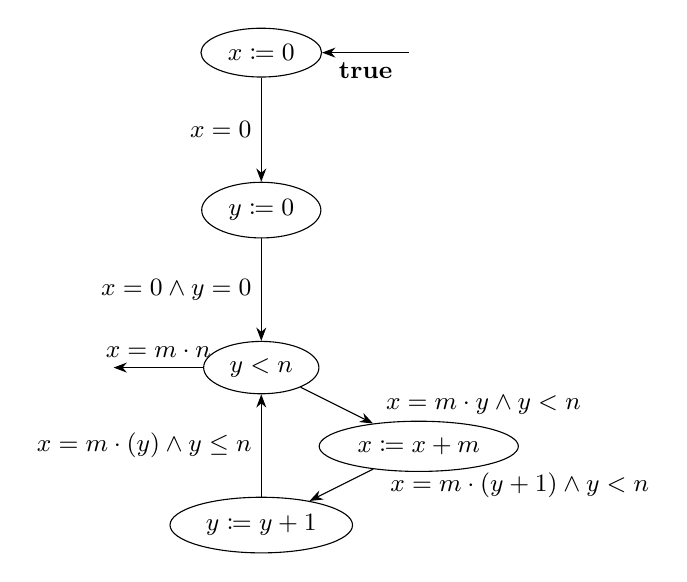
\begin{tikzpicture}[->, >=Stealth]

% Nodes as ellipses
\node (0) at (2, 0) {};
\node (A) [draw, shape=ellipse] at (0, 0) {\small$x\coloneqq0$};
\node (B) [draw, shape=ellipse] at (0, -2) {\small$y\coloneqq0$};
\node (C) [draw, shape=ellipse] at (0, -4) {\small$y<n$};
\node (D) [draw, shape=ellipse] at (2, -5) {\small$x\coloneqq x+m$};
\node (E) [draw, shape=ellipse] at (0, -6) {\small$y\coloneqq y+1$};
\node (1) at (-2, -4) {};
% Edges
\draw (0) -- (A) node[midway, below] {\small $\true$};
\draw (C) -- (1) node[midway, above] {\small$x=m\cdot n$};
\draw (A) -- (B) node[midway, left] {\small$x=0$};
\draw (B) -- (C) node[midway, left] {\small$x=0\land y=0$};
\draw (C) -- (D) node[midway, right=0.5cm] {\small$x=m\cdot y \land y<n$};
\draw (D) -- (E) node[midway, right=0.5cm] {\small$x=m\cdot (y+1) \land y<n$};
\draw (E) -- (C) node[midway, left] {\small$x=m\cdot (y) \land y\leq n$};

\end{tikzpicture}
 \end{center}

\end{example}

 \begin{algorithm}[!h]
    \caption{A program that computes $m* n$}\label{alg:cap}
    \begin{algorithmic}
    \State $\{\true\}$
    \State $x \coloneqq 0$
    \State $\{x=0\}$
    \State $y \coloneqq 0$
    \State $\{x=0 \land y=0\}$
    \While{$y \leq n$} \Comment{loop invariant: $\{x=m* y \land y\leq n\}$}
        \State $\{x = m* y \land y < n\}$
        \State $x \coloneqq x + m$
        \State $\{x = m* (y+1) \land y < n\}$
        \State $y \coloneqq y + 1$
    \EndWhile
    \State $\{x = m* n\}$
    \end{algorithmic}
\end{algorithm}

% \subsection{Flow Chart (Control Flow Graph - ``Floyd Style")}
%     The annotations for the same example can be seen in Figure \ref{cf16}.
% \begin{figure*}[h!]
%     \begin{center}
%     \includegraphics[width=\linewidth]{images/cf16.png}
%     \caption{Control flow graph of the program that computes $x = m * n$.}
%     \end{center}
%     \label{cf16}
% \end{figure*}

\begin{definition}[General Verification Conditions]
    In general, we can derive verification conditions using the following rules:
\begin{itemize}
    \item $\vc(\{\varphi\} ~\simp{{\sskip}}~ \{\psi\}) = \{\varphi \simplies \psi\}$.
    \item $\vc(\{\varphi\} ~\simp{x=a}~ \{\psi\}) = \{\varphi \simplies \psi[x \mapsto a]\}$.
    \item $\vc(\{\varphi\} ~\simp{c_1}~ \{\chi\} ~\simp{ c_2 }~ \{\psi\}) = \vc(\{\varphi\}~\simp{c_1}~ \{\chi\})\,  \cup \, \vc(\{\chi\} ~\simp{c_2}~ \{\psi\})$.
    \item $\vc(\{\varphi\} ~\sif{\simp{b}}{\simp{c_1}}{\simp{c_2}}~ \{\psi\}) = \vc(\{\varphi\land b\} ~\simp{c_1}~ \{\psi\}) \cup \vc(\{\varphi \land \neg b\}~\simp{c_2}~ \{\psi\})$.
    \item $\vc(\{\varphi\} \swhile{\simp{b}}{\simp{c}} \{\psi\}) = \{\varphi \simplies \chi, \chi \land \neg b \simplies \psi\} \cup \vc(\{\chi \land b\} ~\simp{c}~ \{\chi\})$.
\end{itemize}
\end{definition}



\subsection{Programs as predicate transforming (Dijkstra): Weakest (liberal) preconditions}

\begin{definition}[Weakest Liberal Preconditions] $\wlp(\simp{c}, \psi)$ is the \textit{weakest} $\varphi$ s.t $\{\varphi\} ~\simp{c}~ \{\psi\}$, i.e., for all $\varphi$ with $\{\varphi\} ~\simp{c}~\{\psi\}$ we have $ \varphi \simplies \wlp(\simp{c}, \psi)$.
\end{definition}

\begin{definition}[Weakest Preconditions] $\wsp(\simp{c}, \psi)$ is the \textit{weakest} $\varphi$ s.t $\{\varphi\} ~\simp{c}~ \{\psi\} \land \forall \sigma,$ if $\sigma \models \varphi$ then $\simp{c}$ terminates from $\sigma$.
\end{definition}

\begin{definition}
    An assertion language is \emph{expressive} if $\wlp(\simp{c},\psi) = \{\sigma \in \Sigma \mid \sop{c}{\sigma} = \bot \lor \forall \interp. \sde{c}{\sigma} \models_{\interp}\psi\}$.
\end{definition}

\begin{remark}
    For IMP, arithmetic $(\mathbb{N}, +, *)$ is expressive (proof by Goedelization of program executions).
\end{remark}


\begin{example} 
A few examples:
\begin{align*}
    \wlp(\sskip, \psi) &= \psi\\
    \wlp(\simp{x=a}, \psi) &= \psi[x\mapsto a]\\
    \wlp(\simp{c_1}, \simp{c_2}, \psi) &= \wlp(\simp{c_1}, \wlp(\simp{c_1}, \psi)) \\
    \wlp(\simp{\sif{b}{c_1}{c_2}}, \psi) &= (b\simplies \wlp(\simp{c_1}, \psi)) \land (\neg b \simplies \wlp(\simp{c_2}, \psi))\\
    &= (b \land \wlp(\simp{c_1}, \psi)) \lor (\neg b \land \wlp(\simp{c_2}, \psi)) \\
    \wlp(\simp{\swhile{b}{c}}, \psi)  &= \text{weakest} \; \chi:
    \chi \land b \simplies \wlp(\simp{c}, \chi) \land \chi \land \neg b \simplies \psi \\
    \wsp(\simp{\swhile{b}{c}}, \psi)  &= \text{weakest} \; \chi:
    \chi \land b \land (e=n) \simplies \wlp(\simp{c}, \chi\land e>n) \\
    &\quad\quad  \land \chi \land \neg b \simplies \psi \\
    &\quad \quad \land \chi\simplies  e \in \text{well-founded set}
\end{align*}
where $n$ is a fresh variable. 
    % \begin{itemize}
    %     \item $\wlp(\texttt{while } b \texttt{ do } c, \psi) = \texttt{weakest }\chi$ s.t 1) $\chi \land b \simplies \wlp(c, \chi)$ and 2) $\chi \land \neg b \simplies \psi$.
    %     \item For a fresh variable $n$, $\wsp(\texttt{while } b \texttt{ do } \simp{c}, \psi) = \texttt{weakest }\chi$ s.t for a fresh variable $n$ 1) $\chi \land b \land e = n \simplies \wlp(\simp{c}, \chi \land e > n)$, 2) $\chi \land \neg b \simplies \psi$, and 3) $\chi \simplies e \in $ well founded set.
    % \end{itemize}
\end{example}


{{%Localize command definitions

% "empty vertical rectangle" macro by campa		
\newcommand*{\vor}{{\;\setlength{\fboxsep}{0pt}\fbox{\phantom{l}}\;}}


\begin{definition}[$\sassert$ and $\sskip$]
    We define $\sassume$ and $\sskip$ using various semantics.
 \begin{align*}
         \eval{\sskip} &\coloneq \lambda \sigma . \sigma \\
        \eval{\simp{\sassert \; b}} &\coloneq \lambda \sigma . \sif{\simp{b}}{\sigma}{\sfail}\\
    \end{align*}
    and 
    \begin{center}
    \AxiomC{$\langle \simp{b}, \sigma \rangle \downarrow \top$}
    \UnaryInfC{$\langle \simp{\sassert \; b}, \sigma \rangle \downarrow \sigma$}
    \DisplayProof 
    $\quad$
    \AxiomC{$\langle \simp{b}, \sigma \rangle \downarrow \bot$}
    \UnaryInfC{$\langle \simp{\sassert \; b}, \sigma \rangle \downarrow \sfail$}
    \DisplayProof
\end{center}
and 
\begin{align*}
     \wlp(\sskip, \psi) &\coloneqq \psi \\
    \wlp(\simp{\sassert \; b}, \psi) &\coloneqq \simp{b} \land \psi \\
\end{align*}
and 
\begin{center}
   \AxiomC{}
    \UnaryInfC{$ \{ \simp{b} \land \psi \} \sassert \; \simp{b}~ \{ \psi \} $}
    \DisplayProof
\end{center}
Moreover, we can define 
\begin{align*}
      \eval{\simp{c}}\colon \Sigma \to \Sigma_\bot , \quad
        \eval{\simp{c}}\colon \Sigma \to \Sigma_{\bot}^{\sfail} \quad \text{or} \quad   \eval{\simp{c}}\colon \Sigma \times \Sigma_{\bot}^{\sfail}
\end{align*}
for $\Sigma_{\bot}^{\sfail} \coloneq \Sigma_{\{\sfail, \bot\}}$.
\end{definition}



\begin{remark}
    In nondeterministic settings, the symbol $\downarrow$ means ``can reach''.
\end{remark}



\begin{remark}
   The relational semantics generalizes to non-determinism 
\end{remark}

   
\begin{definition}[$\sassume$]
We define $\sassume$ using various semantics.
\begin{align*}
    \eval{\simp{\sassume \; b}} &\coloneq\{ (\sigma, \sigma') \;|\; \sigma \models \simp{b} \land \sigma' = \sigma \}
\end{align*}
and 
\begin{align*}
    \wlp(\simp{\sassume \; b}, \psi) \coloneqq (b\simplies \psi)
\end{align*}
and 
\begin{center}
   \AxiomC{}
    \UnaryInfC{$ \{ \simp{b} \simplies \psi \} \sassume \; \simp{b}~ \{ \psi \} $}
    \DisplayProof
\end{center}
\end{definition}

\begin{definition}
\begin{align*} 
        \wlp(\simp{c}, \psi) \coloneq  \{ \sigma \;|\; \forall \sigma'. (\sigma, \sigma') \in 
\eval{\simp{c}}\simplies \sigma' \models \psi \}
    \end{align*}
\end{definition}


\begin{definition}
    If the assert is false we define 
    \begin{align*}
    \eval{\sabort}  \coloneq \lambda \sigma . \sfail \quad \text{and} \quad  \eval{\simp{havoc \; b}} \coloneq \{ (\sigma, \sigma') \;|\; \sigma' \models\simp{ b} \} 
    \end{align*}
\end{definition}


% Operationally:
% $$\inferrule
% { \langle b, \sigma \rangle \downarrow \top }
% { \langle \textup{assert } b, \sigma \rangle \downarrow \sigma }
% $$



% $$\inferrule
% { \langle b, \sigma \rangle \downarrow \bot }
% { \langle \textup{assert } b, \sigma \rangle \downarrow \sfail }
% $$



% $$ \textup{wlp} ( \textup{assert } b, \psi) = b \wedge \psi $$

% $$ \{ b \wedge \psi \} \textup{ assert } b~ \{ \psi \} $$

% $$ \llbracket c \rrbracket \subseteq \Sigma \times \Sigma_\bot^\sfail $$

% $$ \llbracket \textup{assume } b \rrbracket = \{ (\sigma, \sigma') \;|\; \sigma \vDash b \wedge \sigma' = \sigma \} $$

% We define:
% $$ \textup{wlp} ( c, \psi ) = \psi = \{ \sigma \;|\; \forall \sigma'. (\sigma, \sigma') \in 
% \llbracket c \rrbracket \implies \sigma' \vDash \psi \} $$

% $$ \textup{wlp} ( \textup{assume } b, \psi) = b \implies \psi $$

% $$ \{ b \implies \psi \} \textup{ assume } b~ \{ \psi \} $$

% Assert false:
% $$ \llbracket \textup{abort} \rrbracket = \lambda \sigma . \sfail $$

% $$ \llbracket \textup{havoc } b \rrbracket =  \{ (\sigma, \sigma') \;|\; \sigma' \vDash b \} $$

\subsection{Disjkstra's guarded commands}


\begin{definition}[Syntax]
    Disjkstra's guarded commands are defined by the following grammar
    \begin{align*}
         \sgc &\Coloneqq \overbrace{\ssb \to \ssc}^{\ssb \text{ guard}} \; \mid \;  \overbrace{\sgc \vor \sgc}^{\vor \text{ alternatively}} \\
         \ssc &\Coloneqq \sskip \; \mid \; \sabort \; \mid \; \simp{x} \coloneqq \simp{a} \; \mid \; \ssc; \ssc \; \mid \; \siffi{\sgc} \; \mid \; \sdo{\sgc}
    \end{align*}
\end{definition}

\begin{example}
    Intuitively: We say $\ssb$ is a ``guard'' and we say $\vor$ means ``alternatively''. For example:
    $ x \leq 5 \to x \coloneq x + 1 \vor x \geq 5 \to x \coloneq x - 1 $
\end{example}

\begin{definition}[Rules]
    The behavior of Disjkstra's guarded commands is given by the following inference rules.
    \begin{center}
    \AxiomC{$\langle \ssb, \sigma \rangle \downarrow \top$}
    \AxiomC{$\langle \ssc, \sigma \rangle \downarrow \sigma'$}
    \BinaryInfC{$\langle \ssb \rightarrow \ssc, \sigma \rangle \downarrow \sigma'$}   
    \DisplayProof
    $\quad$
     \AxiomC{$\langle \ssb, \sigma \rangle \downarrow \bot$}
    \UnaryInfC{$\langle \ssb \rightarrow \ssc, \sigma \rangle \downarrow \sfail$}
    \DisplayProof  
    \end{center}
    \begin{center}
         \AxiomC{$\langle \sgc_1, \sigma \rangle \downarrow \sigma'$}
        \UnaryInfC{$\langle \sgc_1 \lor \sgc_2, \sigma \rangle \downarrow \sigma'$}
        \DisplayProof
        $\quad$
        \AxiomC{$\langle \sgc_2, \sigma \rangle \downarrow \sigma'$}
    \UnaryInfC{$\langle \sgc_1 \lor \sgc_2, \sigma \rangle \downarrow \sigma'$}
    \end{center}
    \begin{center}
    \AxiomC{$\langle \sgc_1, \sigma \rangle \downarrow \sfail$}
    \AxiomC{$\langle \sgc_2, \sigma \rangle \downarrow \sfail$}
    \BinaryInfC{$\langle \sgc_1 \lor \sgc_2, \sigma \rangle \downarrow \sfail$}
     \DisplayProof
    \end{center}
    \begin{center}
    \AxiomC{$\langle \sgc, \sigma \rangle \downarrow \sigma'$}
    \UnaryInfC{$\langle \siffi{\sgc}, \sigma \rangle \downarrow \sigma'$}
        \DisplayProof
        $\quad$
    \AxiomC{$\langle \sgc, \sigma \rangle \downarrow \sfail$}
    \UnaryInfC{$\langle \siffi{\sgc}, \sigma \rangle \downarrow \sfail$}
     \DisplayProof
    \end{center}
    \begin{center}
 \AxiomC{$\langle \sgc, \sigma \rangle \downarrow \sfail$}
    \UnaryInfC{$\langle \sdo{\sgc}, \sigma \rangle \downarrow \sigma$}
        \DisplayProof
        $\quad$
    \AxiomC{$\langle \sgc, \sigma \rangle \downarrow \sigma'$}
    \AxiomC{$\langle \sdo{\sgc}, \sigma' \rangle \downarrow \sigma''$}
    \BinaryInfC{$\langle \sdo{\sgc}, \sigma \rangle \downarrow \sigma''$}
     \DisplayProof
    \end{center}
\end{definition}

\begin{example}
    Euclid(gcd): $\sdo{ x > y \to x := x - y \vor y > x \to y := y - x } $

\end{example}


\begin{definition}
    \label{cl17:def:hw}
    We define the grammar
        \begin{align*}
         \ssc &\Coloneqq \sskip \; \mid \;  \simp{x} \coloneqq \simp{a} \; \mid \; \ssc; \ssc \; \mid \; 
         \underbrace{\simp{b} ?}_{\text{assume}\; \ssb} \; \mid \; \underbrace{ \ssc_1 + \ssc_2}_{\text{alternative}} \; \mid \; \underbrace{ \ssc^*}_{\text{iterate $0$ or more}}
    \end{align*}
\end{definition}

\begin{example}
    We can define $\swhile{\ssb}{\ssc}$ by $(\ssb?; \ssc)^*+(\neg \ssb ?)$.
\end{example}

\begin{exercise}
    Give the operational rules, the $\wlp$ definition (or the Hoare rules), and the denotational definition of $\eval{\ssc}$. Moreover, what is $F$ in $\eval{\ssc^*}= \lfp F$.
\end{exercise}
% $$\inferrule
% { \langle b, \sigma \rangle \downarrow \top \\ \langle c, \sigma \rangle \downarrow \sigma' }
% { \langle b \rightarrow c, \sigma \rangle \downarrow \sigma' }
% $$

% $$\inferrule
% { \langle b, \sigma \rangle \downarrow \bot }
% { \langle b \rightarrow c, \sigma \rangle \downarrow \sfail }
% $$

% $$\inferrule
% { \langle \sgc_1, \sigma \rangle \downarrow \sigma' }
% { \langle \sgc_1 \vor \sgc_2, \sigma \rangle \downarrow \sigma' }
% $$

% $$\inferrule
% { \langle \sgc_2, \sigma \rangle \downarrow \sigma' }
% { \langle \sgc_1 \vor \sgc_2, \sigma \rangle \downarrow \sigma' }
% $$

% $$\inferrule
% { \langle \sgc_1, \sigma \rangle \downarrow \sfail \\
%   \langle \sgc_2, \sigma \rangle \downarrow \sfail }
% { \langle \sgc_1 \vor \sgc_2, \sigma \rangle \downarrow \sigma' \sfail }
% $$

% $$\inferrule
% { \langle \sgc, \sigma \rangle \downarrow \sigma' }
% { \langle \siffi{\sgc}, \sigma \rangle \downarrow \sigma' }
% $$

% $$\inferrule
% { \langle \sgc, \sigma \rangle \downarrow \sfail }
% { \langle \siffi{\sgc}, \sigma \rangle \downarrow \sfail }
% $$

% $$\inferrule
% { \langle \sgc, \sigma \rangle \downarrow \sfail }
% { \langle \sdo{\sgc}, \sigma \rangle \downarrow \sigma }
% $$

% $$\inferrule
% { \langle \sgc, \sigma \rangle \downarrow \sigma' \\
%   \langle \sdo{\sgc}, \sigma' \rangle \downarrow \sigma'' }
% { \langle \sdo{\sgc}, \sigma \rangle \downarrow \sigma'' }
% $$


\section{Parallelism}

\begin{example}
    The expression 
         $ x := 0 \parallel x := 1 $ is either $(x := 0;\; x := 1)$ or $(x := 1;\; x := 0)$
\end{example}


\begin{remark}
 Parallelism as nondeterministic interleaving of atomic actions (programs): (i) nondeterministic; (ii) noncompositional; (iii) nonterminating ``reactive programs''. The study of parallelism falls under concurrency theory and process algebra. Here the operator $\parallel$ is added to languages.
    There were dozens of process algebras in the 1990s.
\end{remark}




\subsection{CCS (Calculus of Communicating Systems) by Milner}


\begin{definition}[Syntax]
    We talk about: processes $P$, $Q$; nil $0$ (like skip);  atomic actions $a, b, \dots, \in A$;
    prefix $a.P$ (like sequencing); alternative $P + Q$; process definitions $C \hat{=} P$; 
    parallelism $P \parallel Q$; restriction: $(\nu a) P$; 
\end{definition}

\begin{example}
    We can formulate constructs such as $\mathrm{Iterate} = a.\mathrm{Iterate} +b 0$
\end{example}

\begin{definition}[Structured Operational Semantics]
    The (single-step) structured operational semantics (SOS) of CCS is given by the rules
    \begin{center}
        \AxiomC{}
        \UnaryInfC{$a.P \xrightarrow{a} P$}
        \DisplayProof
        $\quad$
        \AxiomC{$ P \xrightarrow{a} P' $}
        \UnaryInfC{$ P+Q \xrightarrow{a} P'$}
        \DisplayProof
        $\quad$
        \AxiomC{$Q \xrightarrow{a} Q' $}
        \UnaryInfC{$P+Q \xrightarrow{a} Q'$}
        \DisplayProof
        $\quad$
        \AxiomC{$ P \xrightarrow{a} P' $}
        \RightLabel{$C\hat{=}P$}
        \UnaryInfC{$C \xrightarrow{a} P' $}
        \DisplayProof
        $\quad$
    \end{center}
    \begin{center}
        \AxiomC{$ P \xrightarrow{a} P' $}
        \UnaryInfC{$ P \parallel Q \xrightarrow{a} P' \parallel Q$}
        \DisplayProof
        $\quad$
        \AxiomC{$  Q \xrightarrow{a} Q' $}
        \UnaryInfC{$  P \parallel Q \xrightarrow{a} P \parallel Q' $}
        \DisplayProof
    \end{center}
        \begin{center}
        \AxiomC{$  P \xrightarrow{a} P' $}
        \AxiomC{$   Q \xrightarrow{\bar{a}} Q' $}
        \BinaryInfC{$  P \parallel Q \xrightarrow{\tau} P' \parallel Q' $}
        \DisplayProof
        $\quad$
        \AxiomC{$  P \xrightarrow{b} P' $}
        \RightLabel{$ a \neq b,\, \bar{a} \neq b$}
        \UnaryInfC{$ (\nu a) P \xrightarrow{b} (\nu a) P' $}
        \DisplayProof
    \end{center}
\end{definition}

\begin{example}
    Sequential Processes are action labeled directed graphs, i.e., a labeled transition system. For example $c \hat{=} ab 0 + acd C$ corresponds to the graph
     \begin{center}
 
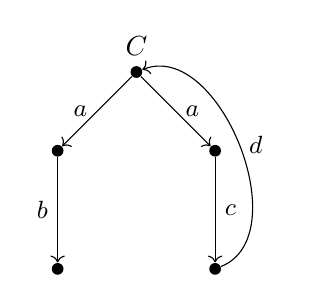
\begin{tikzpicture}[scale=1]

    % Graph nodes
    \node[circle, fill, inner sep=1.5pt, label=above:{$C$}] (0) at (0,0) {};
    \node[circle, fill, inner sep=1.5pt] (a1) at (-1,-1) {};
    \node[circle, fill, inner sep=1.5pt] (a2) at (-1,-2.5) {};
    \node[circle, fill, inner sep=1.5pt] (b1) at (1,-1) {};
    \node[circle, fill, inner sep=1.5pt] (b2) at (1,-2.5) {};

    % Edges with labels
    \draw[->] (0) to node[midway, left] {\small$a$} (a1);
    \draw[->] (0) to node[midway, right] {\small$a$} (b1);
    \draw[->] (a1) to node[midway, left] {\small$b$} (a2);
    \draw[->] (b1) to node[midway, right] {\small$c$} (b2);
    \draw[bend right=90, ->] (b2) to node[midway, right] {\small$d$} (0);

\end{tikzpicture}
 
 \end{center}
\end{example}




\begin{definition}
 Let $A$ be a set of atomic actions.
 For each $a \in A$ we denote $a!$ as send $a$ and $a?$ as receive $a$.
 Then a sequential process and a concurrent process is given by the respective grammars 
 \begin{align*}
     P & \Coloneqq 0 \;|\; a.P \;|\; P + P && \text{(sequential process)} \\
    P & \Coloneqq P \;|\; Q \parallel  Q \;|\; (\nu a) Q  \;|\; C && \text{(concurrent process)} \\
 \end{align*}
 where $C$ is a process constant.
 If $\nu$ is omitted then we obtain a BPP ("basic parallel processes").
 Note: the binding strength of the operators are $\nu > . > \parallel  > +$; $.$ and $0$ are often omitted.
 \end{definition}
 
%  $P := O | a.P | P + P$
% \end{definition}
% \begin{itemize}
% 	\item set $A$ of atomic actions.
% 	\item 
% 	\item sequential processes $P := O | a.P | P + P$
% 	\item concurrent processes $Q := P | Q \parallel  Q | (\nu a) Q | C \text{(process constant)}$
% \end{itemize}

\begin{definition}[CCS network]
    A CCS network $\ccs$ is a (possibly infinite) set of equations that define process constants such that every constant that occurs in $\ccs$: 
    (i) is defined by an equation in $\ccs$; 
    (ii) every r.h.s. occurrence is "guarded" i.e. occurs within an action prefix.
\end{definition}

\begin{example}
	$$\{C_0 = a.C_1 + b.O, C_1 = a.C_0 \parallel bbaO\}$$
\end{example}

\begin{definition}[Semantics]
    The semantics of CCS is given by the following rules. We define $\tau$ as a fixed operator symbol and $\mu$ as a meta-variable representing any action (including $\tau$).
    \begin{center}
        \AxiomC{}
        \UnaryInfC{$ aP \xrightarrow{a} P $}
        \DisplayProof
      \quad
     \AxiomC{$P \xrightarrow{\mu} P'$}
     \RightLabel{$\mu \neq a!, a?$}
    \UnaryInfC{$(\nu a)P \xrightarrow{\mu}(\nu a)P'$}
     \DisplayProof
    \end{center}
    \begin{center}
    \AxiomC{$P \xrightarrow{a} P'$}
    \UnaryInfC{$ P + Q \xrightarrow{a} P' + Q $}
    \noLine
    \UnaryInfC{$ Q + P \xrightarrow{a} Q + P' $}
    \noLine
    \UnaryInfC{$ P\parallel Q \xrightarrow{a} P'\parallel Q $}
    \noLine
    \UnaryInfC{$ Q\parallel P \xrightarrow{a} Q\parallel P' $}
    \DisplayProof
    \quad
     \AxiomC{$P \xrightarrow{a?} P' $}
    \AxiomC{$Q \xrightarrow{a!} Q'$}
    \BinaryInfC{$ P\parallel Q \xrightarrow{\tau} P' \parallel  Q'$}
     \noLine
    \UnaryInfC{$ Q \parallel  P \xrightarrow{\tau} Q' \parallel  P'$}
     \DisplayProof
    \end{center}
\end{definition}


% %without $\nu$: BPP ("basic parallel processes")
% CCS network  = set of equations that define process constants st. every constant that occurs in P:
% i) is defined by an equation in P
% ii) every r.h.s. occurrence is "guarded" i.e. occurs within an action prefix



\begin{example}[Vending Machine]
\label{cl18:ex:ccs1}
The $\ccs$ for a coffee and tea vending machine consists of the following equations
\begin{align*}
     V &= \coin? (\reqcof? \discof! V + \reqtea? \distea!V), \\
     C &= \coin! \reqcof! \discof? C,  \\
     S &= (\nu \coin)(\nu \reqcof)(\nu \reqtea, \distea, \discof) V \parallel C
\end{align*}
constructed over the set $A = \{\coin, \reqcof, \reqtea, \discof, \distea\}$ of atomic actions.
 \begin{center}
 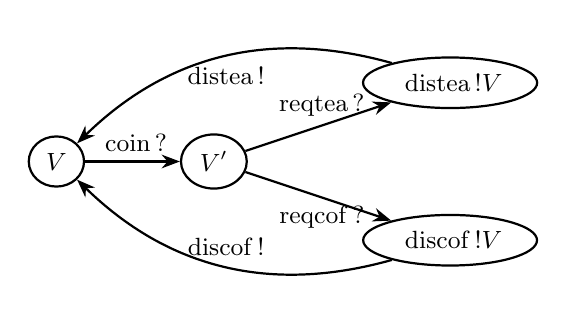
\begin{tikzpicture}[->, >=Stealth, node distance=2cm, thick, main/.style = {draw, ellipse}]
    % Nodes
   
    \node[main] (1) at (0, 0) {\small$V$};
    \node[main] (2) at (2, 0) {\small$V'$};
    \node[main] (3) at (5, 1) {\small$\distea!V$};
    \node[main] (4) at (5, -1) {\small$\discof!V$};

    % Edges
    \draw  (1) to node[midway, above] {\small$\coin?$} (2) ;
    \draw  (2) to node[midway, above] {\small$\reqtea?$} (3) ;
    \draw  (2) to node[midway, below] {\small$\reqcof?$} (4);
    \draw[bend right] (3) to node[midway, below] {\small$\distea!$} (1) ;
    \draw[bend left] (4) to node[midway, above] {\small$\discof!$} (1);
\end{tikzpicture}
 \end{center}
 The interface $S$ of $V$ is given as the graph
  \begin{center}
 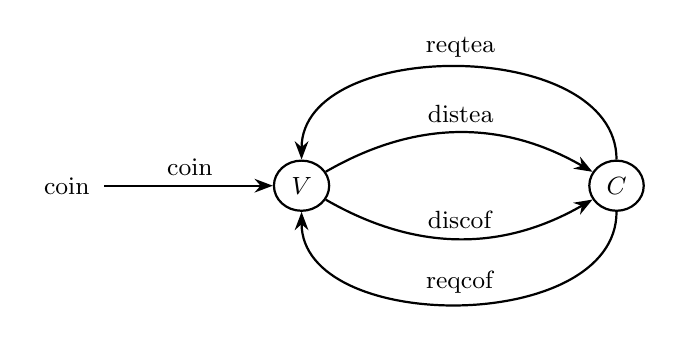
\begin{tikzpicture}[->, >=Stealth, node distance=2cm, thick, main/.style = {draw, ellipse}]
    % Nodes
    \node (0) at (-3, 0) {\small$\coin$};
    \node[main] (1) at (0, 0) {\small$V$};
    \node[main] (2) at (4, 0) {\small$C$};

    % Edges
    \draw  (0) to node[midway, above] {\small$\coin$} (1) ;
    \draw[bend left]  (1) to node[midway, above] {\small$\distea$} (2) ;
    \draw[bend right]  (1) to node[midway, above] {\small$\discof$} (2) ;
    \draw[bend right=90]  (2) to node[midway, above] {\small$\reqtea$} (1) ;
    \draw[bend left=90]  (2) to node[midway, above] {\small$\reqcof$} (1) ;
  
\end{tikzpicture}
 \end{center}

   \begin{center}
 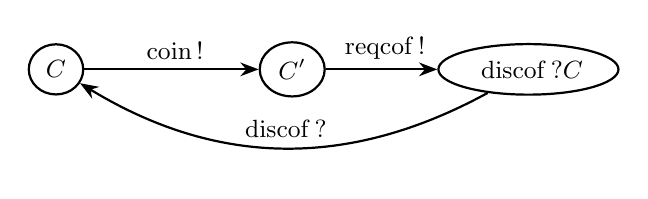
\begin{tikzpicture}[->, >=Stealth, node distance=2cm, thick, main/.style = {draw, ellipse}]
    % Nodes
  
    \node[main] (1) at (0, 0) {\small$C$};
    \node[main] (2) at (3, 0) {\small$C'$};
    \node[main] (3) at (6, 0) {\small$\discof?C$};

    % Edges
    \draw  (1) to node[midway, above] {\small$\coin!$} (2) ;
     \draw  (2) to node[midway, above] {\small$\reqcof!$} (3) ;
    \draw[bend left]  (3) to node[midway, above] {\small$\discof?$} (1) ;


\end{tikzpicture}
 \end{center}



   \begin{center}
 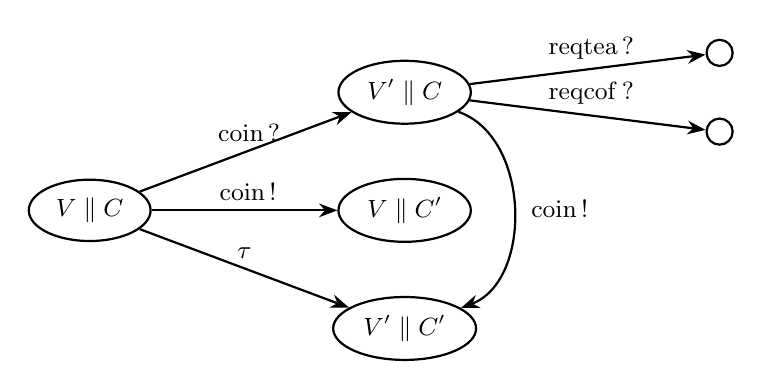
\begin{tikzpicture}[->, >=Stealth, node distance=2cm, thick, main/.style = {draw, ellipse}]
    % Nodes
  
    \node[main] (11) at (0, 0) {\small$V\parallel C$};
    \node[main] (21) at (4, 1.5) {\small$V'\parallel C$};
    \node[main] (22) at (4, 0) {\small$V\parallel C'$};
    \node[main] (23) at (4, -1.5) {\small$V'\parallel C'$};
    
    \node[main] (31) at (8, 2) {};
    \node[main] (32) at (8, 1) {};

    
     \draw  (11) to node[midway, above] {\small$\coin?$} (21) ;
     \draw  (11) to node[midway, above] {\small$\coin!$} (22) ;
     \draw  (11) to node[midway, above] {\small$\tau$} (23) ;

    \draw  (21) to node[midway, above] {\small$\reqtea?$} (31) ;
     \draw  (21) to node[midway, above] {\small$\reqcof?$} (32) ;
     \draw[bend left=70]  (21) to node[midway, right] {\small$\coin!$} (23) ;

    % Edges
    % \draw  (1) to node[midway, above] {\small$\coin!$} (2) ;
    %  \draw  (2) to node[midway, above] {\small$\reqcof!$} (3) ;
    % \draw[bend left]  (3) to node[midway, above] {\small$\discof?$} (1) ;


\end{tikzpicture}
 \end{center}

   \begin{center}
 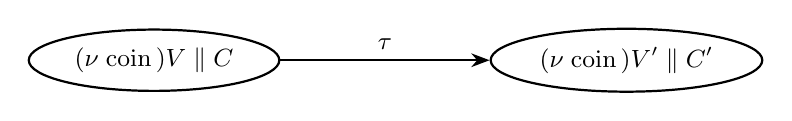
\begin{tikzpicture}[->, >=Stealth, node distance=2cm, thick, main/.style = {draw, ellipse}]
    % Nodes
  
    \node[main] (1) at (0, 0) {\small$(\nu \coin)V\parallel C$};
    \node[main] (2) at (6, 0) {\small$(\nu \coin)V'\parallel C'$};

    % Edges
    \draw  (1) to node[midway, above] {\small$\tau$} (2) ;
    
\end{tikzpicture}
 \end{center}

\begin{center}
 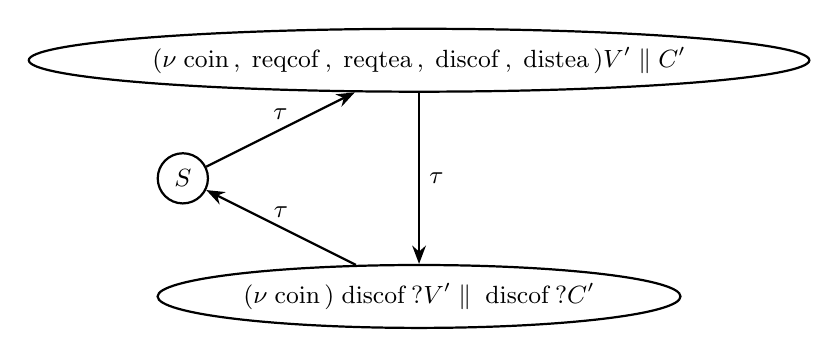
\begin{tikzpicture}[->, >=Stealth, node distance=2cm, thick, main/.style = {draw, ellipse}]
    % Nodes
  
    \node[main] (1) at (0, 0) {\small$S$};
    \node[main] (2) at (3, 1.5) {\small$(\nu \coin, \reqcof, \reqtea, \discof, \distea)V'\parallel C'$};
    \node[main] (3) at (3, -1.5) {\small$(\nu \coin)\discof?V'\parallel \discof?C'$};

    % Edges
    \draw  (1) to node[midway, above] {\small$\tau$} (2) ;
    \draw  (2) to node[midway, right] {\small$\tau$} (3) ;
    \draw  (3) to node[midway, above] {\small$\tau$} (1) ;
\end{tikzpicture}
 \end{center}
	% interface of V: in figure \ref{lec18:pic1}.
	% \begin{figure}[h]
	% 	\label{lec18:pic1}
	% 	\centering
	% 	\includegraphics[width=0.7\linewidth]{images/1.png}
	% 	\includegraphics[width=0.7\linewidth]{images/2.png}
	% 	\caption{Interface of V}
	% \end{figure}
\end{example}





\begin{remark}
     CCS networks are Turing-complete but finite CCS networks are still infinite state but not Turing-complete.
\end{remark}

\begin{example}[Counter]
    Let $A \coloneq \{\inc, \dec, \zero\}$, then we define 
    \begin{align*}
        \Counter\coloneqq \left\{
            \begin{array}{l}
                C_0 = \inc?C_1 + \zero? C_0, \\
                C_1 = \inc?C_2 + \dec? C_0, \\
               C_2 = \inc?C_3 + \dec? C_1, \\
               \vdots
            \end{array}
        \right\}
    \end{align*}  
    and 
    \begin{align*}
        \semicounter \coloneq \{SC = \inc?(SC\parallel \dec?0)\}
    \end{align*}
   \begin{center}
 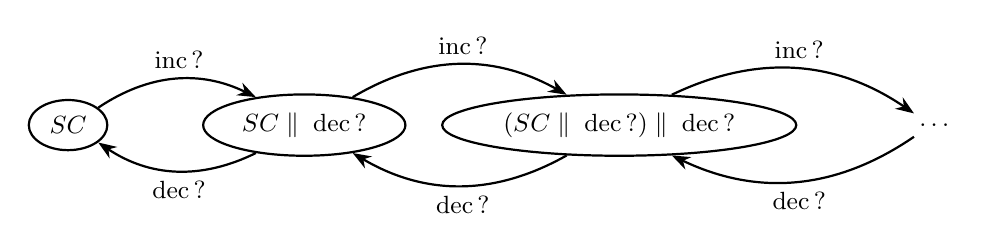
\begin{tikzpicture}[->, >=Stealth, node distance=2cm, thick, main/.style = {draw, ellipse}]
    % Nodes
  
    \node[main] (1) at (0, 0) {\small$SC$};
    \node[main] (2) at (3, 0) {\small$SC\parallel\dec?$};
    \node[main] (3) at (7, 0) {\small$(SC\parallel\dec?)\parallel\dec?$};
    \node (4) at (11, 0) {\small$\hdots$};

    % Edges
    \draw[bend left]  (1) to node[midway, above] {\small$\inc?$} (2) ;
    \draw[bend left]  (2) to node[midway, below] {\small$\dec?$} (1) ;
    \draw[bend left]  (2) to node[midway, above] {\small$\inc?$} (3) ;
    \draw[bend left]  (3) to node[midway, below] {\small$\dec?$} (2) ;
    \draw [bend left] (3) to node[midway, above] {\small$\inc?$} (4) ;
    \draw[bend left]  (4) to node[midway, below] {\small$\dec?$} (3) ;
   


\end{tikzpicture}
 \end{center}
\end{example}


\begin{definition}[Regular CCS Network]
    Regular (finite) CCS networks are defined by the following grammar. 
    Regular networks are finite state.
    \begin{align*}
        R &\Coloneqq O \;\mid\;  aP \;\mid\; R + R \\
        P &\Coloneqq R \;\mid\; C \\
        Q &\Coloneqq  P \;\mid\; Q \parallel  Q \;\mid\; (\nu a) Q
    \end{align*}
\end{definition}

\begin{remark}
    Regular CCS networks represent a finite set of CCS processes, each parallel composition of (possibly nested) sequential processes.
\end{remark}




\begin{theorem}[Laws]
For an appropriately chosen notion of equivalence, the following equation hold
\begin{align*}
    P + Q  &\approx Q + P, \; \\
    (P + Q) + R &\approx P + (Q + R), \;\\
    P + P &\approx P, \; \\
    P + O &\approx P
\end{align*}
In addition we have the \emph{expansion law}
\begin{align*}
    a \parallel  b \approx ab + ba
\end{align*}
\end{theorem}



\section{Labeled Transition Systems}

\begin{definition}[Labeled Transition Systems]
    A labeled transition systems (LTS) for a set of actions $A$ is a tuple $T\coloneqq (S, \to, )$ where $S$ is a set of states, and $\to \subseteq S\times A \times S$ is a labeled transition relation. It defines a finite or infinite directed graph whose edges are labeled by actions (including $\tau$ which is an invisible action).
\end{definition}


\begin{example}
    A process network $\mathcal{P}$ can be encoded as a LTS $T_{\mathcal{P}}$.
    We define $S$ to be the set of sub-processions that occur in  $\mathcal{P}$ closed under $\to$ and 
    $\to$ is given by the SOS rules. 
\end{example}


\begin{remark}
    A LTS $T=(S, \to)$ is finitely branching (for guarded process terms) if $A$ is finite and finite state if $S$ is finite. 
\end{remark}





\begin{exercise}
	Design a coffee machine that needs refilling after every second drink, together with a coffee preferring customer, and a second tea preferring customer that never refills. Give CCS network and the corresponding LTS (for all sub-processions).
\end{exercise}





% \begin{tikzpicture}[->, >=Stealth, node distance=2cm, thick, main/.style = {draw, circle}]
%     % Nodes
%     \node[main] (1) {A};
%     \node[main] (2) [below right of=1] {B};
%     \node[main] (3) [below left of=2] {C};
%     \node[main] (4) [below right of=2] {D};

%     % Edges
%     \draw[bend left] (1) to node[midway, above left] {2} (2);
%     \draw[bend left] (1) to node[midway, above right] {3} (3);
%     \draw[bend left] (2) to node[midway, below left] {1} (3);
%     \draw[bend left] (2) to node[midway, above right] {4} (4);
%     \draw[bend left] (3) to node[midway, below right] {5} (4);
% \end{tikzpicture}



% \paragraph{semanitcs}:
% $$\frac{}{aP \xrightarrow{a} P}$$
% $$\frac{P \xrightarrow{a} P'}{P + Q \xrightarrow{a} P' + Q, Q + P \xrightarrow{a} Q + P', P\parallel Q \xrightarrow{a} P'\parallel Q, Q\parallel P \xrightarrow{a} Q\parallel P'}$$
% $$\frac{P \xrightarrow{a?} P', Q \xrightarrow{a!} Q'}{P\parallel Q \xrightarrow{\tau} P' \parallel  Q', Q \parallel  P \xrightarrow{\tau} Q' \parallel  P'}$$ where $\tau$ is a fixed operator symbol
% $$\frac{P \xrightarrow{\mu} P'}{(\nu a)P \xrightarrow{\mu}(\nu a)P'}\mu \neq a!, a?$$ where $\mu$ is a meta variable standing for any action, including $\tau$

% \begin{example}
% 	continuation ...
	
% 	In figure \ref{lec18:pic2}.
% 	\begin{figure}[h]
% 		\label{lec18:pic2}
% 		\centering
% 		\includegraphics[width=0.7\linewidth]{images/3.png}
% 		\caption{Semantic of V}
% 	\end{figure}
% \end{example}



% \begin{example}
	
	
% 	counter =
% 	$\{C_0 = inc?C_1 + zero? C_0, C_1 = inc?C_2 + dec? C_0, C_2 = inc? C_3 + dec? C_1, ...\}$
	
% 	semi-counter:
% 	$\{SC = inc? (SC \parallel  dec?O)\}$
	
% 	See figure \ref{lec18:pic3}.
% 	\begin{figure}[h]
% 		\label{lec18:pic3}
% 		\centering
% 		\includegraphics[width=0.7\linewidth]{images/4.png}
% 		\caption{Counter model}
% 	\end{figure}
% \end{example}



% Note:

% \paragraph{Regular finite CCS networks}
% $$R:= O | aP |R + R$$
% $$P := R | C$$
% $$Q :=  | Q \parallel  Q | (\nu a) Q$$

% finite set of CCS processes, each a parallel comb of seq processes.
% The regular networks are finite state.

% \begin{exercise}
% 	design a coffee machine that needs refilling after every second drink, together with a coffee preferring customer, and a second tea preferring customer that never refills. Give CCS network  + corresponding LTS (for all subprocessions)
% \end{exercise}



% \paragraph{"Laws" (equations)}
% $$ P + Q  \approx Q + P$$
% $$(P + Q) + R \approx P + (Q + R)$$
% $$P + P \approx P$$
% $$P + O \approx P$$

% Expansion law (simple form): $a \parallel  b \approx ab + ba$

% \subsection{LTS}
% LTS (for set $A$ of actions) $T = (S\text{(states)}, \rightarrow (subset S\times A \times S),)$
% finite or infinite directed graph whose edges are labeled by actions (including $\tau$(invisible action))

% Process network P $\rightarrow$ LTS $T_P$: 
% i) S = set of subprocessions that occur in P closed under $\rightarrow$, and ii) $\rightarrow$ = defined by SOS rules


% \paragraph{4 equivalence relations on LTS}
% \begin{itemize}
% 	\item $\eqiso$: isomorphism between LTS
% 	\item $\eqbis$: bisimilarity
% 	\item $\eqsim$: similarity
% 	\item $\eqlin$: language equivalance
% \end{itemize}

% Note: upper ones can result lower, but not the other way around.




% \documentclass{article}
% \usepackage{graphicx} % Required for inserting images
% \usepackage{pbox}
% \usepackage{amsmath,amssymb,amsfonts,amsthm,mathptmx}
% \usepackage{stmaryrd}
% 

%%%%%% Basic Math
\newcommand{\comment}[1]{\textcolor{red}{#1}}

\newcommand{\notimplies}{%
  \mathrel{{\ooalign{\hidewidth$\not\phantom{=}$\hidewidth\cr$\implies$}}}}


\newcommand{\RN}{\mathbb{R}}
\newcommand{\QN}{\mathbb{Q}}
\newcommand{\NN}{\mathbb{N}}
\newcommand{\BN}{\mathbb{B}}
\newcommand{\ZN}{\mathbb{Z}}
\newcommand{\power}{\mathcal{P}}

\newcommand{\true}{\mathbf{true}}
\newcommand{\false}{\mathbf{false}}


\newcommand{\simplies}{\Rightarrow}
\newcommand{\simplied}{\Leftarrow}
\newcommand{\siff}{\Leftrightarrow}
\newcommand{\emptystring}{\epsilon}
\newcommand{\gfp}{\mathrm{gfp}}
\newcommand{\lfp}{\mathrm{lfp}}
\newcommand{\bottom}{\perp}

\newcommand{\valfoo}{\nu}
\newcommand{\eval}[1]{\llbracket #1 \rrbracket}
\newcommand{\interp}{\mathcal{I}}

\newcommand{\sat}{\mathbf{sat}}
\newcommand{\unsat}{\mathbf{unsat}}
%%%%%% Merge Sort

\newcommand{\mergesort}{\mathtt{mergesort}}
\newcommand{\merges}{\mathtt{merge}}
\newcommand{\odd}{\mathtt{odd}}
\newcommand{\even}{\mathtt{even}}
\newcommand{\sorted}{\mathtt{sorted}}
\newcommand{\reverseA}{\mathtt{reverse}}
\newcommand{\reverseB}{\mathtt{reverse2}}

\newcommand{\parent}{\mathtt{parent}}
\newcommand{\monkey}{\mathtt{monkey}}
\newcommand{\human}{\mathtt{human}}


\newcommand{\proofs}{\vdash}


\newcommand{\hilbert}{\mathcal{H}}
% \newcommand{\nj}{\mathcal{N}\mkern-9mu\mathcal{J}}
% \newcommand{\nk}{\mathcal{N}\mkern-6mu\mathcal{K}}
% \newcommand{\lk}{\mathcal{L}\mkern-6mu\mathcal{K}}
\newcommand{\nj}{\mathcal{NJ}}
\newcommand{\nk}{\mathcal{NK}}
\newcommand{\lk}{\mathcal{LK}}
 
\newcommand{\kripke}{m}
\newcommand{\krel}{\preceq}
\newcommand{\kinit}{w_0}
\newcommand{\kworld}{W}


\newcommand{\lif}{\mathrm{if}}
% \newcommand{\ln}{\underline{if}}


\newcommand{\tuple}[1]{\langle #1 \rangle}

\newcommand{\sif}[3]{\mathrm{if}\;#1\;\mathrm{then}\;#2\;\mathrm{else}\;#3}
\newcommand{\swhile}[2]{\mathrm{while}\;#1\;\mathrm{do}\;#2}
\newcommand{\siffi}[1]{\mathrm{if}\;#1\;\mathrm{fi}}
\newcommand{\sdo}[1]{\mathrm{do}\;#1\;\mathrm{od}}
\newcommand{\sskip}{\mathtt{skip}}
\newcommand{\sassert}{\mathtt{assert}}
\newcommand{\sfail}{\mathtt{fail}}
\newcommand{\sassume}{\mathtt{assume}}
\newcommand{\sabort}{\mathtt{abort}}
\newcommand{\ssc}{\mathtt{c}}
\newcommand{\ssb}{\mathtt{b}}
\newcommand{\sgc}{\mathtt{gc}}

\newcommand{\simp}[1]{\mathtt{#1}}
\newcommand{\sop}[2]{\langle \simp{#1},~#2 \rangle}
\newcommand{\sde}[1]{\llbracket \simp{#1} \rrbracket}
\newcommand{\sdefun}[1]{\lambda \sigma.~ #1}

\newcommand{\imp}[1]{\texttt{#1}}
\newcommand{\opsem}[2]{\langle \imp{#1},~#2 \rangle}
\newcommand{\desem}[1]{\llbracket \imp{#1} \rrbracket}
\newcommand{\defun}[1]{\lambda \sigma.~ #1}



\newcommand{\vc}{\mathrm{vc}}
\newcommand{\wlp}{\mathrm{wlp}}
\newcommand{\wsp}{\mathrm{wp}}



\newcommand{\ccs}{\mathcal{P}}

\newcommand{\coin}{\;\mathrm{coin}\,}
\newcommand{\discof}{\;\mathrm{discof}\,}
\newcommand{\reqcof}{\;\mathrm{reqcof}\,}
\newcommand{\distea}{\;\mathrm{distea}\,}
\newcommand{\reqtea}{\;\mathrm{reqtea}\,}


\newcommand{\inc}{\;\mathrm{inc}\,}
\newcommand{\dec}{\;\mathrm{dec}\,}
\newcommand{\zero}{\;\mathrm{zero}\,}
\newcommand{\Counter}{\;\mathrm{Counter}\,}
\newcommand{\semicounter}{\;\mathrm{Semicounter}\,}



\newcommand{\equiso}{\approx_{\mathrm{iso}}}
\newcommand{\equbis}{\approx_{\mathrm{bis}}}
\newcommand{\equsim}{\approx_{\mathrm{sim}}}
\newcommand{\equlin}{\approx_{\mathrm{lin}}}

\newcommand{\lequsim}{\preceq_{\mathrm{sim}}}
\newcommand{\gequsim}{\succeq_{\mathrm{sim}}}

\providecommand{\T}{T}
\DeclareMathOperator{\pre}{pre}
\DeclareMathOperator{\post}{post}
\DeclareMathOperator{\HML}{HML}
\DeclareMathOperator{\HMLlin}{HML_{\mathrm{lin}}}



\newcommand{\bev}[1]{\langle #1 \rangle}
\newcommand{\bal}[1]{[ #1 ]}

\newcommand{\lev}{\lozenge}
\newcommand{\lal}{\square}
\newcommand{\lne}{\bigcirc}
\newcommand{\lun}{\,\mathcal{U}\,}

\newcommand{\lmu}{\mu\,}
\newcommand{\lnu}{\nu\,}

\newcommand{\algo}{\mathcal{A}}


\newcommand{\tatom}{\mathrm{atom}}
\newcommand{\tcar}{\mathrm{car}}
\newcommand{\tcdr}{\mathrm{cdr}}
\newcommand{\tcons}{\mathrm{cons}}

\newcommand{\tread}{\mathrm{read}}
\newcommand{\twrite}{\mathrm{write}}


% \title{Formalisms Every Computer Scientist Should Know}
% \author{Lecture 19}
% \date{\today}

% \begin{document}

% \maketitle
% \section{}


\begin{example}
\label{cl19:ex:equ}
When are two processes equal? For example consider the following syntactic CCS expressions
\begin{align*}
    P=a(bP + c), \quad P'=bP+c, \text{and} \quad P''=c+bP
\end{align*}
To answer this we look at their semantics, which is given by LTS, e.g., 
   \begin{center}
 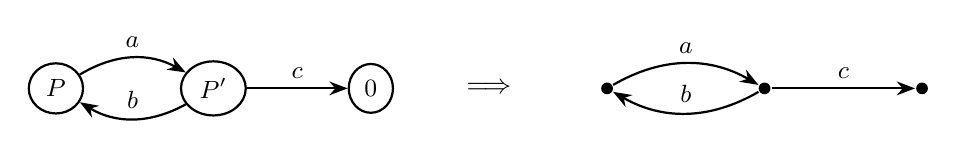
\begin{tikzpicture}[->, >=Stealth, node distance=2cm, thick, 
    main/.style = {draw, ellipse}, 
    dot/.style = {circle, fill, inner sep=1.5pt}]
    % Nodes
  
    \node[main] (1) at (0, 0) {\small$P$};
    \node[main] (2) at (2, 0) {\small$P'$};
    \node[main] (3) at (4, 0) {\small$0$};

    \node[dot] (4) at (7, 0) {};
    \node[dot] (5) at (9, 0) {};
    \node[dot] (6) at (11, 0) {};

    \node (0) at (5.5, 0) {$\implies$};
    % Edges
    \draw[bend left] (1) to node[midway, above] {\small$a$} (2) ;
     \draw  (2) to node[midway, above] {\small$c$} (3) ;
    \draw[bend left]  (2) to node[midway, above] {\small$b$} (1) ;

    \draw[bend left]  (4) to node[midway, above] {\small$a$} (5) ;
    \draw  (5) to node[midway, above] {\small$c$} (6) ;
    \draw[bend left]  (5) to node[midway, above] {\small$b$} (4) ;

\end{tikzpicture}
 \end{center}
 Hence, the question can be reduced to defining equivalences between LTS.
\end{example}



 
\begin{definition}[Equivalences]
    the four common equivalence relations on LTS are: 
    (i) $\equiso$ isomorphism between LTS; 
    (ii) $\equbis$ bisimilarity;
    (iii) $\equsim$ similarity;
    (iv) $\equlin$ language equivalence.
\end{definition}

\begin{theorem}
    We know that:
    \begin{align*}
        \equiso &\implies  \equbis \implies  \equsim \implies  \equlin \\
        \equlin &\notimplies  \equsim \notimplies  \equbis \notimplies  \equiso
    \end{align*}
\end{theorem}


\begin{definition}[Isomorphism]
Let $T_1 = (S_1,\mapsto)$ and $T_2 = (S_2,\mapsto)$. Let $s_1 \in S_1$ and $s_2 \in S_2$. Then $s_1 \equiso s_2$ iff there exists $h: S_1 \mapsto S_2$ such that:
\setlist{nolistsep}
\begin{enumerate}[(i), noitemsep]
    \item $h$ is a bijection (onto and 1-1);
    \item for all $s,s' \in S_1$ and all actions $a \in A$, we have $s \xrightarrow{a} s'$ iff $h(s) \xrightarrow{a} h(s')$;
    \item $h(s_1) = s_2$.
\end{enumerate}
% (i) $h$ is a bijection (onto and 1-1); (ii) for all $s,s' \in S_1$ and all actions $a \in A$, we have $s \xrightarrow{a} s'$ iff $h(s) \xrightarrow{a} h(s')$; $h(s_1) = s_2$.
\end{definition}

\begin{remark}
    Isomorphism can be seen as a structural equivalence. 
\end{remark}


\begin{example}[Ex.~\ref{cl19:ex:equ} cont.]
    It is easy to see that  $P' \equiso P''$ due to the commutativity of $+$, i.e., $P+Q=Q+P$. 
    However, this notion of equivalence is too strong to capture $P=P+P$, i.e., semantically $P$ and $P+P$ can be represented  as
    
    \begin{center}
    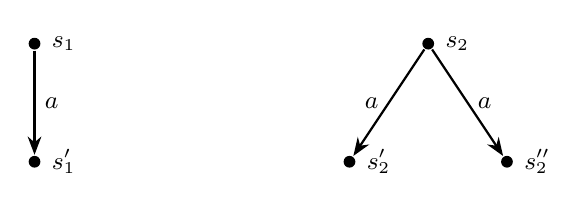
\begin{tikzpicture}[->, >=Stealth, node distance=2cm, thick, 
    main/.style = {draw, ellipse}, 
    dot/.style = {circle, fill, inner sep=1.5pt}]
    % Nodes

    \node[dot, label=right:{\small$s_1$}] (1) at (0, 0) {};
    \node[dot, label=right:{\small$s_1'$}] (2) at (0, -1.5) {};

    
    \node[dot, label=right:{\small$s_2$}] (4) at (5, 0) {};
    \node[dot, label=right:{\small$s_2'$}] (5) at (4, -1.5) {};
    \node[dot, label=right:{\small$s_2''$}] (6) at (6, -1.5) {};

    % Edges
  
    \draw  (1) to node[midway, right] {\small$a$} (2) ;
    \draw  (4) to node[midway, left] {\small$a$} (5) ;
    \draw  (4) to node[midway, right] {\small$a$} (6) ;
    

\end{tikzpicture}
 \end{center}
 As there is no bijection to be found the two LTS are not isomorphic. Hence, we are interested in weaker notions of similarity. 
\end{example}


\begin{definition}[Bisimilarity]
    Let $T_1 = (S,\mapsto)$. Let $s_1 \in S$ and $s_2 \in S$. Then $s_1 \equbis s_2$ iff there exists $r \subseteq S \times S$ such that:
    \setlist{nolistsep}
    \begin{enumerate}[(i),noitemsep]
        \item $ \forall s_1,s_2\in S$ if  $(s_1,s_2) \in r$, then $\forall s_1' \in S, \forall a\in A$ if $s_1 \xrightarrow{a} s_1'$ then $\exists s_2'$ such that $s_2 \xrightarrow{a} s_2'$ and $(s_1',s_2') \in r$;
        \item $\forall s_1,s_2$ if $(s_1,s_2) \in r$, then $\forall s_2'\in S, \forall a \in A$ if $s_2 \xrightarrow{a} s_2'$, then $\exists$ $s_1'$ such that $s_1 \xrightarrow{a} s_1'$ and $(s_1',s_2') \in r$; 
        \item $(s_1,s_2) \in r$.
    \end{enumerate}
\end{definition}

\begin{example}[Ex.~\ref{cl19:ex:equ} cont.]
    Continuing. While $P$ and $P+P$ are not isomorphic, they are bisimilar, i.e., we define $r\coloneqq \{(s_1, s_2), (s_1',s_2'), (s_1',s_2'')\}$
    \begin{center}
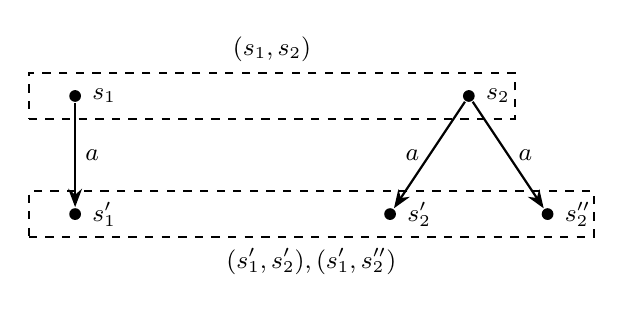
\begin{tikzpicture}[->, >=Stealth, node distance=2cm, thick, 
    main/.style = {draw, ellipse}, 
    dot/.style = {circle, fill, inner sep=1.5pt}]
    % Nodes

    \node[dot, label=right:{\small$s_1$}] (1) at (0, 0) {};
    \node[dot, label=right:{\small$s_1'$}] (2) at (0, -1.5) {};

    \node[dot, label=right:{\small$s_2$}] (4) at (5, 0) {};
    \node[dot, label=right:{\small$s_2'$}] (5) at (4, -1.5) {};
    \node[dot, label=right:{\small$s_2''$}] (6) at (6, -1.5) {};

    % Edges
    \draw  (1) to node[midway, right] {\small$a$} (2) ;
    \draw  (4) to node[midway, left] {\small$a$} (5) ;
    \draw  (4) to node[midway, right] {\small$a$} (6) ;

    % Boxes around top and bottom nodes
    \node[draw, dashed, fit=(1)(4), label=above:{\small$(s_1, s_2)$}, inner xsep=5mm, inner ysep=2mm] {};
    \node[draw, dashed, fit=(2)(5)(6), label=below:{\small$(s_1', s_2'), (s_1', s_2'')$}, inner xsep=5mm, inner ysep=2mm] {};

\end{tikzpicture}
 \end{center}
\end{example}

\begin{remark}
    Both the identity and all graph isomorphism are bisimulations. The converse does not hold. 
    Computing isomorphisms is hard, i.e., it is somewhere between $\mathrm{P}$ and $\mathrm{NP}$. Whereas computing bisimulations is relatively easy, i.e., $\mathcal{O}(m\log n)$ where $n$ is the number of states and $m$ the number of edges. 
\end{remark}

% \begin{itemize}
%     \item 
%     \item the opposite of the above is not true
%     \item computing isomorphisms is hard 
%     \item computing bisimilarity is "easy" $O(m \log n)$ where $m$ is the number of edges and $n$ is number of states.
% \end{itemize} 

\begin{theorem}
    \label{cl19:thrm:bis}
    Let $r \subseteq S\times S$ and let 
    \begin{align*}
        C_{(i)}(r,s_1, s_2)&\coloneqq \forall s_1' \forall a.\;  s_1 \xrightarrow{a} s_1' \simplies \exists s_2'.\;  s_2 \xrightarrow{a} s_2' \wedge r(s_1',s_2') \\
        C_{(ii)}(r,s_1, s_2)&\coloneqq \forall s_2' \forall a .\; s_2 \xrightarrow{a} s_2' \simplies \exists s_1'.\;  s_1 \xrightarrow{a} s_1' \wedge r(s_1',s_2') \}
    \end{align*}
    We define $F(r) = \{(s_1,s_2) | C_{(i)}(r,s_1, s_2) \land C_{(ii)}(r,s_1, s_2)\}$. 
    Then $\equbis = \gfp F$.
\end{theorem}

\begin{remark}
    From Theorem \ref{cl19:thrm:bis} we can derive a simple algorithm for computing $\equbis$ by starting from $S\times S$ and iteratively refining the relation. 
    \begin{align*}
        && \equbis^{0} &= S\times S \\
       &\supseteq & \equbis^{1} &= F(\equbis^{0}) =  \{(s_1,s_2) | C_{(i)}(\equbis^{0},s_1, s_2) \land C_{(ii)}(\equbis^{0},s_1, s_2)\}\\ 
       & \supseteq & \equbis^{2} &= F(\equbis^{1}) =  \{(s_1,s_2) | C_{(i)}(\equbis^{1},s_1, s_2) \land C_{(ii)}(\equbis^{1},s_1, s_2)\}\\ 
        &\supseteq & \vdots \\
        & \supseteq & \equbis &= \gfp F(S\times S)
    \end{align*}
    This is called the simple fixed-point approximation algorithm (aka. partition refinement): $O(m\cdot n)$
\end{remark}


\begin{example}
    Consider the following LTS
    \begin{center}
 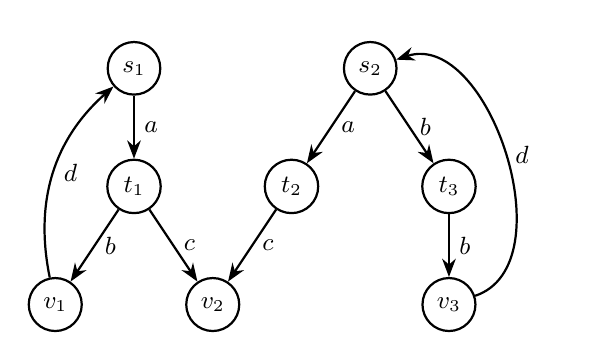
\begin{tikzpicture}[->, >=Stealth, node distance=2cm, thick, main/.style = {draw, circle},
    dot/.style = {circle, fill, inner sep=1.5pt}]
    % Nodes
    \node[main] (s1) at (0, 0) {\small$s_1$};
    \node[main] (s2) at (3, 0) {\small$s_2$};
    \node[main] (t1) at (0, -1.5) {\small$t_1$};
    \node[main] (t2) at (2, -1.5) {\small$t_2$};
    \node[main] (t3) at (4, -1.5) {\small$t_3$};
    \node[main] (v1) at (-1, -3) {\small$v_1$};
    \node[main] (v2) at (1, -3) {\small$v_2$};
    \node[main] (v3) at (4, -3) {\small$v_3$};

    \draw (s1) to node[midway, right] {\small$ a $} (t1) ;
    \draw (t1) to node[midway, right] {\small$ b $} (v1) ;
    \draw (t1) to node[midway, right] {\small$ c $} (v2) ;
    \draw[bend left] (v1) to node[midway, right] {\small$ d $} (s1) ;

    \draw (s2) to node[midway, right] {\small$ a $} (t2) ;
    \draw (s2) to node[midway, right] {\small$ b $} (t3) ;
    \draw (t2) to node[midway, right] {\small$ c $} (v2) ;
    \draw (t3) to node[midway, right] {\small$ b $} (v3) ;
    \draw[bend right=90] (v3) to node[midway, right] {\small$ d $} (s2) ;
   
    % \node[main] (2) at (2, 0) {\small$V'$};
    % \node[main] (3) at (5, 1) {\small$\distea!V$};
    % \node[main] (4) at (5, -1) {\small$\discof!V$};

    % % Edges
    % \draw  (1) to node[midway, above] {\small$\coin?$} (2) ;
    % \draw  (2) to node[midway, above] {\small$\reqtea?$} (3) ;
    % \draw  (2) to node[midway, below] {\small$\reqcof?$} (4);
    % \draw[bend right] (3) to node[midway, below] {\small$\distea!$} (1) ;
    % \draw[bend left] (4) to node[midway, above] {\small$\discof!$} (1);
\end{tikzpicture}
 \end{center}
 Then applying the fixed-point approximation algorithm we get 
\begin{align*}
       \equbis^{0} &= S\times S \\
       \equbis^{1} &=   \mathrm{id} \cup \{ (v_1,v_2), (v_1, v_3), (v_2, v_1), (v_2, v_3), (v_3,v_1),(v_3, v_2)\}\\ 
      & \vdots\\
      \equbis &=   \mathrm{id} \cup \{(v_1, v_2), (v_2, v_1)\}
\end{align*}
where $\mathrm{id}\coloneqq \{(s_1,s_1), (s_2,s_2), (t_1,t_1), (t_2,t_2), (t_3,t_3), (v_1,v_1), (v_2,v_2), (v_3,v_3)
\}$ is the identity relation.
\end{example}
% \textbf{Algorithm.} Let $r \in S\times S$ and define $F(r) = \{(s_1,s_2) | \textit{1. and 2. from definition of bisimilarity}\}$. 

% It holds that $\sim_{bis} = \mathit{gfp}~ F$. 

% \begin{align*}
%     \sim_{bis}^0 &= S \times S \\
%     \sim_{bis}^1 &= F(\sim_{bis}^0) = \{(s_1,s_2)| & \forall s_1', s_1 \xrightarrow{a} s_1' \Rightarrow \exists s_2'; s_2 \xrightarrow{a} s_2' \wedge \sim_{bis}^0(s_1',s_2') \\ 
%     & & \wedge  \forall s_2', s_2 \xrightarrow{a} s_2' \Rightarrow \exists s_1'; s_1 \xrightarrow{a} s_1' \wedge \sim_{bis}^0(s_1',s_2') \}
% \end{align*}
% This is called the simple fixed-point approximation algorithm (aka. partition refinement): $O(m.n)$

\begin{definition}[Simulation]
    \label{cl19:def:sim}
    For $s_1,s_2 \in S$, $s_2$ simulates $s_1$, i.e., $s_1 \lequsim s_2$, iff $\exists r \in S \times S$ such that:
    \setlist{nolistsep}
    \begin{enumerate}[(i),noitemsep]
        \item $\forall s_1,s_2$ if $s_1 \lequsim  s_2$ then, $\forall s_1' \forall a$  if $s_1 \xrightarrow{a} s_1'$ then $\exists s_2'$ such that $s_2 \xrightarrow{a} s_2'$ and $s_1' \lequsim  s_2'$;
        \item $(s_1,s_2) \in r$
    \end{enumerate}
\end{definition}

\begin{remark}
    Note that in Definition \ref{cl19:def:sim} the second condition in bisimilarity is not present in the definition of simulation. (Example on difference on blackboard)
    Hence, it is not symmetric.
\end{remark}

\begin{example}
    The asymmetry of $\lequsim$ can be observed in the following example. The right structure simulates the left, but the inverse does not hold.
    \begin{center}
    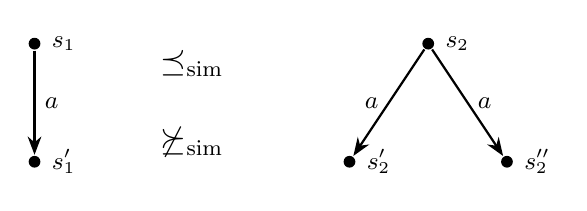
\begin{tikzpicture}[->, >=Stealth, node distance=2cm, thick, 
    main/.style = {draw, ellipse}, 
    dot/.style = {circle, fill, inner sep=1.5pt}]
    % Nodes

    \node[dot, label=right:{\small$s_1$}] (1) at (0, 0) {};
    \node[dot, label=right:{\small$s_1'$}] (2) at (0, -1.5) {};


    \node (b) at (2,-0.25) {\large$\lequsim$};
    \node (a) at (2, -1.25) {\large$\not\gequsim$};
    
    \node[dot, label=right:{\small$s_2$}] (4) at (5, 0) {};
    \node[dot, label=right:{\small$s_2'$}] (5) at (4, -1.5) {};
    \node[dot, label=right:{\small$s_2''$}] (6) at (6, -1.5) {};

    % Edges
  
    \draw  (1) to node[midway, right] {\small$a$} (2) ;
    \draw  (4) to node[midway, left] {\small$a$} (5) ;
    \draw  (4) to node[midway, right] {\small$a$} (6) ;
    

\end{tikzpicture}
 \end{center}
\end{example}


\begin{definition}[Similarity]
    Two states $s_1,s_2$ are called similar or $s_1 \equsim s_2$ iff (i) $s_1 \lequsim  s_2$ and (ii) $s_2 \lequsim  s_1$.
\end{definition}

\begin{remark}
    Bisimilarity implies similarity, but the opposite direction is not generally true.
    Similarity is a greatest fixed-point and can be computed via approximation sequence $\equsim^0, \equsim^1, \dots$ in $\mathcal{O}(m\cdot n)$.
\end{remark}

\begin{example}
    The following demonstrates that similartiy is a weaker form of equivalence than bisimulation. 
        \begin{center}
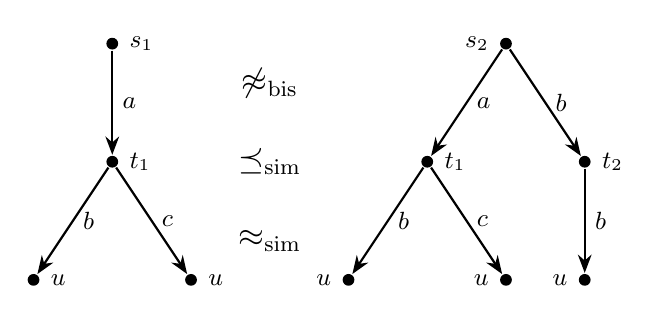
\begin{tikzpicture}[->, >=Stealth, node distance=2cm, thick, 
    main/.style = {draw, circle}, dot/.style = {circle, fill, inner sep=1.5pt}]
    
    % Nodes with labels to the right
    \node[dot, label=right:{\small$s_1$}] (s1) at (0, 0) {};
    \node[dot, label=left:{\small$s_2$}] (s2) at (5, 0) {};
    \node[dot, label=right:{\small$t_1$}] (t1) at (0, -1.5) {};
    \node[dot, label=right:{\small$t_1$}] (t2) at (4, -1.5) {};
    \node[dot, label=right:{\small$t_2$}] (t3) at (6, -1.5) {};
    \node[dot, label=right:{\small$u$}] (v1) at (-1, -3) {};
    \node[dot, label=right:{\small$u$}] (v2) at (1, -3) {};
    \node[dot, label=left:{\small$u$}] (v3) at (3, -3) {};
    \node[dot, label=left:{\small$u$}] (v4) at (5, -3) {};
    \node[dot, label=left:{\small$u$}] (v5) at (6, -3) {};

    \node (b) at (2,-0.5) {\large$\not\equbis$};
    \node (b) at (2,-1.5) {\large$\lequsim$};
    \node (b) at (2,-2.5) {\large$\equsim$};

    % Edges
    \draw (s1) to node[midway, right] {\small$ a $} (t1) ;
    \draw (t1) to node[midway, right] {\small$ b $} (v1) ;
    \draw (t1) to node[midway, right] {\small$ c $} (v2) ;


    \draw (s2) to node[midway, right] {\small$ a $} (t2) ;
    \draw (s2) to node[midway, right] {\small$ b $} (t3) ;
    \draw (t2) to node[midway, right] {\small$ b $} (v3) ;
    \draw (t2) to node[midway, right] {\small$ c $} (v4) ;
    \draw (t3) to node[midway, right] {\small$ b $} (v5) ;


\end{tikzpicture}
 \end{center}
 in this transition system we have 
 \begin{align*}
     \equbis &= \{(s,s) \mid s\in S\} = \mathrm{id}\\
     \lequsim &= \mathrm{id} \cup \{ (t_2,t_1), (s_1,s_2), (s_2, s_1)\}   \\
      \equsim &=  \mathrm{id} \cup \{ (s_1,s_2), (s_2, s_1)\} \\
 \end{align*}
\end{example}


\begin{theorem}
    \label{cl19:thrm:CCS}
    Bisimilarity is a congruence for CCS, i.e., (i) bisimilarity is an equivalence and (ii) for all CCS processes $P,Q,R$, if $P \equbis Q$ then $R[P] \equbis R[Q]$, e.g., $R+P \equbis R+Q$ or  $R \parallel P \equbis R \parallel Q$
\end{theorem}

\begin{exercise}
    Proof (ii) in Theorem~\ref{cl19:thrm:CCS}.
\end{exercise}
% \end{document} 

% \documentclass{article}
% \usepackage{graphicx} % Required for inserting images


% \renewcommand{\equsim}{\approx_{sim}}
% \providecommand{\equbis}{\approx_{bis}}


% 

%%%%%% Basic Math
\newcommand{\comment}[1]{\textcolor{red}{#1}}

\newcommand{\notimplies}{%
  \mathrel{{\ooalign{\hidewidth$\not\phantom{=}$\hidewidth\cr$\implies$}}}}


\newcommand{\RN}{\mathbb{R}}
\newcommand{\QN}{\mathbb{Q}}
\newcommand{\NN}{\mathbb{N}}
\newcommand{\BN}{\mathbb{B}}
\newcommand{\ZN}{\mathbb{Z}}
\newcommand{\power}{\mathcal{P}}

\newcommand{\true}{\mathbf{true}}
\newcommand{\false}{\mathbf{false}}


\newcommand{\simplies}{\Rightarrow}
\newcommand{\simplied}{\Leftarrow}
\newcommand{\siff}{\Leftrightarrow}
\newcommand{\emptystring}{\epsilon}
\newcommand{\gfp}{\mathrm{gfp}}
\newcommand{\lfp}{\mathrm{lfp}}
\newcommand{\bottom}{\perp}

\newcommand{\valfoo}{\nu}
\newcommand{\eval}[1]{\llbracket #1 \rrbracket}
\newcommand{\interp}{\mathcal{I}}

\newcommand{\sat}{\mathbf{sat}}
\newcommand{\unsat}{\mathbf{unsat}}
%%%%%% Merge Sort

\newcommand{\mergesort}{\mathtt{mergesort}}
\newcommand{\merges}{\mathtt{merge}}
\newcommand{\odd}{\mathtt{odd}}
\newcommand{\even}{\mathtt{even}}
\newcommand{\sorted}{\mathtt{sorted}}
\newcommand{\reverseA}{\mathtt{reverse}}
\newcommand{\reverseB}{\mathtt{reverse2}}

\newcommand{\parent}{\mathtt{parent}}
\newcommand{\monkey}{\mathtt{monkey}}
\newcommand{\human}{\mathtt{human}}


\newcommand{\proofs}{\vdash}


\newcommand{\hilbert}{\mathcal{H}}
% \newcommand{\nj}{\mathcal{N}\mkern-9mu\mathcal{J}}
% \newcommand{\nk}{\mathcal{N}\mkern-6mu\mathcal{K}}
% \newcommand{\lk}{\mathcal{L}\mkern-6mu\mathcal{K}}
\newcommand{\nj}{\mathcal{NJ}}
\newcommand{\nk}{\mathcal{NK}}
\newcommand{\lk}{\mathcal{LK}}
 
\newcommand{\kripke}{m}
\newcommand{\krel}{\preceq}
\newcommand{\kinit}{w_0}
\newcommand{\kworld}{W}


\newcommand{\lif}{\mathrm{if}}
% \newcommand{\ln}{\underline{if}}


\newcommand{\tuple}[1]{\langle #1 \rangle}

\newcommand{\sif}[3]{\mathrm{if}\;#1\;\mathrm{then}\;#2\;\mathrm{else}\;#3}
\newcommand{\swhile}[2]{\mathrm{while}\;#1\;\mathrm{do}\;#2}
\newcommand{\siffi}[1]{\mathrm{if}\;#1\;\mathrm{fi}}
\newcommand{\sdo}[1]{\mathrm{do}\;#1\;\mathrm{od}}
\newcommand{\sskip}{\mathtt{skip}}
\newcommand{\sassert}{\mathtt{assert}}
\newcommand{\sfail}{\mathtt{fail}}
\newcommand{\sassume}{\mathtt{assume}}
\newcommand{\sabort}{\mathtt{abort}}
\newcommand{\ssc}{\mathtt{c}}
\newcommand{\ssb}{\mathtt{b}}
\newcommand{\sgc}{\mathtt{gc}}

\newcommand{\simp}[1]{\mathtt{#1}}
\newcommand{\sop}[2]{\langle \simp{#1},~#2 \rangle}
\newcommand{\sde}[1]{\llbracket \simp{#1} \rrbracket}
\newcommand{\sdefun}[1]{\lambda \sigma.~ #1}

\newcommand{\imp}[1]{\texttt{#1}}
\newcommand{\opsem}[2]{\langle \imp{#1},~#2 \rangle}
\newcommand{\desem}[1]{\llbracket \imp{#1} \rrbracket}
\newcommand{\defun}[1]{\lambda \sigma.~ #1}



\newcommand{\vc}{\mathrm{vc}}
\newcommand{\wlp}{\mathrm{wlp}}
\newcommand{\wsp}{\mathrm{wp}}



\newcommand{\ccs}{\mathcal{P}}

\newcommand{\coin}{\;\mathrm{coin}\,}
\newcommand{\discof}{\;\mathrm{discof}\,}
\newcommand{\reqcof}{\;\mathrm{reqcof}\,}
\newcommand{\distea}{\;\mathrm{distea}\,}
\newcommand{\reqtea}{\;\mathrm{reqtea}\,}


\newcommand{\inc}{\;\mathrm{inc}\,}
\newcommand{\dec}{\;\mathrm{dec}\,}
\newcommand{\zero}{\;\mathrm{zero}\,}
\newcommand{\Counter}{\;\mathrm{Counter}\,}
\newcommand{\semicounter}{\;\mathrm{Semicounter}\,}



\newcommand{\equiso}{\approx_{\mathrm{iso}}}
\newcommand{\equbis}{\approx_{\mathrm{bis}}}
\newcommand{\equsim}{\approx_{\mathrm{sim}}}
\newcommand{\equlin}{\approx_{\mathrm{lin}}}

\newcommand{\lequsim}{\preceq_{\mathrm{sim}}}
\newcommand{\gequsim}{\succeq_{\mathrm{sim}}}

\providecommand{\T}{T}
\DeclareMathOperator{\pre}{pre}
\DeclareMathOperator{\post}{post}
\DeclareMathOperator{\HML}{HML}
\DeclareMathOperator{\HMLlin}{HML_{\mathrm{lin}}}



\newcommand{\bev}[1]{\langle #1 \rangle}
\newcommand{\bal}[1]{[ #1 ]}

\newcommand{\lev}{\lozenge}
\newcommand{\lal}{\square}
\newcommand{\lne}{\bigcirc}
\newcommand{\lun}{\,\mathcal{U}\,}

\newcommand{\lmu}{\mu\,}
\newcommand{\lnu}{\nu\,}

\newcommand{\algo}{\mathcal{A}}


\newcommand{\tatom}{\mathrm{atom}}
\newcommand{\tcar}{\mathrm{car}}
\newcommand{\tcdr}{\mathrm{cdr}}
\newcommand{\tcons}{\mathrm{cons}}

\newcommand{\tread}{\mathrm{read}}
\newcommand{\twrite}{\mathrm{write}}



% \commenter{ruichen}{violet}




% \section{$\equsim$ and $\equbis$}


\begin{definition}
    We define the predecessor and successor of a subset $\sigma\subseteq S$ for some actions $a\in A$ respectively as 
    \begin{align*}
         \pre_a(\sigma) \coloneqq \{ s \mid  \exists s' \in \sigma.\ s \xrightarrow{a} s' \} \\
          \post_a(\sigma) \coloneqq \{ s' \mid \exists s \in \sigma.\ s \xrightarrow{a} s' \} 
    \end{align*}
\end{definition}

\begin{remark}
    The set $\pre_a(\sigma)$ is the set of states that can reach $\sigma$ by action $a$ and the set $\post_a(\sigma)$ is the set of states that can be reached from $\sigma$ by action $a$.
    \begin{center}
         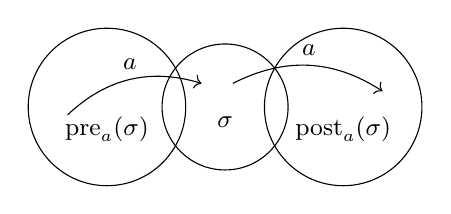
\begin{tikzpicture}
    % Draw the three intersecting circles
    \draw (0,0) circle (1cm) node[below] {\small $ \pre_a(\sigma)$};  % First circle
    \draw (1.5,0) circle (0.8cm) node[below] {\small $\sigma$};  % Center circle
    \draw (3,0) circle (1 cm) node[below] {\small $\post_a(\sigma)$};  % Third circle
    
    % Draw the arrows
    % Arrow from the middle circle to the first circle
    \draw[->, bend left] (-0.5, -0.1) to node[midway, above] {\small$a$}  (1.2, 0.3) ;
    % Arrow from the middle circle to the third circle
    \draw[->,bend left] (1.6, 0.3) to  node[midway, above] {\small$a$}  (3.5, 0.2);
\end{tikzpicture}
    \end{center}
\end{remark}

\begin{theorem}
    \begin{align*}
        s \lequsim t &\iff \exists R \subseteq S \times S.\ (s,t) \in R \simplies \forall a\ \forall s' \in \post_a(s)\ \exists t' \in post_a(t).  (s', t') \in R  \\
          s \equsim t &\iff s \lequsim t \land  t \lequsim s  \\
           s \equbis t &\iff \exists R \subseteq S \times S.\ (s,t) \in R \simplies \forall a\left[
            \begin{array}{l}
               ( \forall s' \in \post_a(s)\ \exists t' \in \post_a(t). (s', t') \in R )\; \land \\
                ( \forall t' \in \post_a(t)\ \exists s' \in \post_a(s). (s', t') \in R )
            \end{array}
        \right]
    \end{align*}
\end{theorem}


\subsection{Characterization}


\begin{theorem}[Game theoretic characterization of $\lequsim$]
The game theoretic characterization  $\lequsim$ is given be the following game.
\begin{enumerate}
    \item Put red token on $s$, and blue token on $t$.
    \item Repeat:
        \begin{enumerate}
            \item Player $1$ moves the \emph{red} token to a successor state.
            \item Player $2$ moves the \emph{blue} button to a successor state, matching the action of the player $1$ move.
        \end{enumerate}
\end{enumerate}
If in the following game player $1$ has a strategy s.t. at some point, player $2$ cannot match player $1$'s move, then $s \not\lequsim t$, otherwise $s \lequsim t$.
\end{theorem}


\begin{theorem}[Game theoretic characterization of $\equbis$]
The game theoretic characterization  $\lequsim$ is given be the following game.
\begin{enumerate}
    \item Put red token on $s$, and blue token on $t$.
    \item Repeat:
        \begin{enumerate}
            \item Player $1$ chooses either the red or blue token.
            \item Player $1$ moves the \emph{chosen} token to a successor state.
            \item Player $2$ moves the \emph{other} button to a successor state, matching the action of the player $1$ move.
        \end{enumerate}
\end{enumerate}
If in the following game player $1$ has a strategy s.t. at some point, player $2$ cannot match player $1$'s move, then $s \not\equbis t$, otherwise $s \equbis t$.
\end{theorem}



% \begin{definition}[Game theoretic of $\equsim$]
% The game theoretic characterization of $\lequsim$ and $\equbis$ is the following.
% For $\lequsim$, if in the following game player $1$ has a strategy s.t. at some point, player $2$ cannot match player $1$'s move, then $s \not\lequsim t$, otherwise $s \lequsim t$.
% \begin{enumerate}
%     \item Put red token on $s$, and blue token on $t$.
%     \item Repeat:
%         \begin{enumerate}
%             \item Player $1$ moves the \emph{red} token to a successor state.
%             \item Player $2$ moves the \emph{blue} button to a successor state, matching the action of the player $1$ move.
%         \end{enumerate}
% \end{enumerate}
% For $\equbis$ the same holds for the following game.
% \begin{enumerate}
%     \item Put red token on $s$, and blue token on $t$.
%     \item Repeat:
%         \begin{enumerate}
%             \item Player $1$ chooses either the red or blue token.
%             \item Player $1$ moves the \emph{chosen} token to a successor state.
%             \item Player $2$ moves the \emph{other} button to a successor state, matching the action of the player $1$ move.
%         \end{enumerate}
% \end{enumerate}
% \end{definition}


% \begin{definition}[Fixpoint of $\equsim$]
% The fixpoint characterization of $\equsim$ and $\equbis$ is the following.
% For 
% For $\lequsim$, if in the following game player $1$ has a strategy s.t. at some point, player $2$ cannot match player $1$'s move, then $s \not\lequsim t$, otherwise $s \lequsim t$.
% \begin{enumerate}
%     \item Put red token on $s$, and blue token on $t$.
%     \item Repeat:
%         \begin{enumerate}
%             \item Player $1$ moves the \emph{red} token to a successor state.
%             \item Player $2$ moves the \emph{blue} button to a successor state, matching the action of the player $1$ move.
%         \end{enumerate}
% \end{enumerate}
% For $\equbis$ the same holds for the following game.
% \begin{enumerate}
%     \item Put red token on $s$, and blue token on $t$.
%     \item Repeat:
%         \begin{enumerate}
%             \item Player $1$ chooses either the red or blue token.
%             \item Player $1$ moves the \emph{chosen} token to a successor state.
%             \item Player $2$ moves the \emph{other} button to a successor state, matching the action of the player $1$ move.
%         \end{enumerate}
% \end{enumerate}
% \end{definition}

% \begin{enumerate}
%     \item Put red token on $s$, and blue token on $t$.
%     \item Repeat:
%         \begin{enumerate}
%             \item ($\equbis$) Player $1$ chooses either red or blue, and moves the chosen token to a successor state. ($\equsim$) Player $1$ moves the red token to a successor state.
%             \item ($\equbis$) Player $2$ moves the other token to a successor state, matching the action of the player $1$ move. ($\equsim$) Player $2$ moves the blue button to a successor state, matching the action of the player $1$ move.
%         \end{enumerate}
% \end{enumerate}




\begin{algorithm}[htp]
\caption{$\algo_{\equbis}$}
\label{alg:bis}
\begin{algorithmic}
    \State $X \gets \{ S \}$
    \State $X' \gets \{ \emptyset\}$
    \While{$X'\not=X$} 
        \State $X' \gets X$
        \State $X \gets X \cup \{ \sigma \cup \pre_a(\sigma') | \sigma, \sigma' \in X,\ a \in A \} \cup \{ \sigma \setminus \pre_a(\sigma') | \sigma, \sigma' \in X,\ a \in A \}$
    \EndWhile
    \If{$\forall \sigma\in X.\; s,t \in \sigma \lor s,t \notin \sigma$ }
        \State \Return $\true$
    \EndIf
    \State \Return $\false$
\end{algorithmic}
\end{algorithm}



\begin{theorem}[Fixpoint characterization of $\equbis$]
        Algorithm $\algo_{\equbis}$ provides a fixed point characterization of $\equbis$, i.e., $\forall s, t\in S$ we have that $s \equbis t$ iff  $\algo_{\equbis}$ terminates with $\true$.
\end{theorem}

\begin{algorithm}[htp]
\caption{$\algo_{\equsim}$}
\label{alg:bis}
\begin{algorithmic}
    \State $X \gets \{ S \}$
    \State $X' \gets \{ \emptyset\}$
    \While{$X'\not=X$} 
        \State $X' \gets X$
        \State $X \gets X \cup \{ \sigma \cup \pre_a(\sigma') | \sigma, \sigma' \in X,\ a \in A \}$
    \EndWhile
    \If{$\forall \sigma\in X.\; s,t \in \sigma \lor s,t \notin \sigma$ }
        \State \Return $\true$
    \EndIf
    \State \Return $\false$
\end{algorithmic}
\end{algorithm}



\begin{theorem}[Fixpoint characterization of $\equsim$]
        Algorithm $\algo_{\equsim}$ provides a fixed point characterization of $\equsim$, i.e., $\forall s, t\in S$ we have that $s \equsim t$ iff  $\algo_{\equsim}$ terminates with $\true$.
\end{theorem}

\begin{definition}[Hennessy-Milner Logic ($\HML$) Syntax]
    The syntax of Hennessy-Milner Logic ($\HML$) is given by the following grammar.
    \begin{align*}
        \varphi \Coloneqq\true  \; \mid \;  \false \; \mid \;  \varphi \land \varphi \; \mid \;  \varphi \lor \varphi \; \mid \;  \bev{a} \varphi  ,\;  a \in A \; \mid \;  \bal{a} \varphi,\;  a \in A
    \end{align*}
    \end{definition}


\begin{definition}[Hennessy-Milner Logic ($\HML$) Semantics]
    The semantics of Hennessy-Milner Logic ($\HML$) is defined as follows. 
    Let $T\coloneqq (S, \to)$ be a labeled transition system, let $\varphi$ a $\HML$ formula, let $s\in S$, then we define $s\models \varphi$ inductively:
    \begin{itemize}[noitemsep]
        \item if $ \varphi = \varphi_1 \land \varphi_2 $, then $ s \models_T \varphi_1 \land \varphi_2$ iff $s \models_T \varphi_1$ and  $\models_T \varphi_2$;
        \item if $ \varphi = \varphi_1 \lor \varphi_2 $, then $ s \models_T \varphi_1 \lor \varphi_2$ iff $s \models_T \varphi_1$ and  $\models_T \varphi_2$;
      \item if $ \varphi = \bev{a}\varphi $, then $ s \models_T\bev{a}\varphi $ iff $\exists s' \in \post_a(s).\ s' \models_T \varphi$ \\
      (equivalent to $\exists s' .\; s \xrightarrow{a} s' \land  \varphi$); 
    \item if $ \varphi = \bal{a}\varphi $, then $ s \models_T\bal{a}\varphi $ iff $\forall s' \in \post_a(s).\ s' \models_T \varphi$ \\
      (equivalent to $\forall s' .\; s \xrightarrow{a} s' \simplies  \varphi$); 
    \end{itemize}
    Moreover, we define $\eval{\varphi}_T\subseteq S$ s.t. $\eval{\true}_T\coloneqq S$, $\eval{\false}_T \coloneqq  \emptyset$, $\eval{\varphi_1 \land \varphi_2}_T \coloneqq  \eval{\varphi_1 }_T \cap \eval{\varphi_2}_T$, and $\eval{\varphi_1 \lor \varphi_2}_T \coloneqq  \eval{\varphi_1 }_T \cup \eval{\varphi_2}_T$.
\end{definition}

\begin{definition}[$\HML$ Fragments]
     The logic $\HML^\exists$ is the $\HML$ without $\bal{a}$. The logic $\HML ^\forall$ is the $\HML$ without $\bev{a}$. The logic $\HML_\neg$ adds negation, i.e., for any $\HML$ formula we add $\neg \varphi$.
\end{definition}

\begin{lemma}
    In $\HML_{\neg}$ the following equivalences hold
    \begin{align*}
        \neg \true &\equiv \false \\
        \neg (\varphi_1 \land \varphi_2) &\equiv \neg \varphi_1 \lor \neg\varphi_2 \\
        \neg \bev{a}\varphi &\equiv \bal{a}\neg \varphi \\
        \neg \bal{a}\varphi &\equiv \bev{a}\neg \varphi \\
    \end{align*}
\end{lemma}

\begin{theorem}[Logical Characterization of $\equbis$]
    The $\equbis$ is logically characterized by $\HML$, i.e.,  $s \equbis t$ iff $\forall \varphi \in \HML$, either $s,t \models \varphi$ or $s,t \not\models \varphi$. 
\end{theorem}

\begin{theorem}[Logical Characterization of $\equsim$]
    The $\equsim$ is logically characterized by $\HML^{\exists}$ (or $\HML^{\forall}$), i.e.,
    $s \equsim t$ iff $\forall \varphi \in \HML ^\exists$, either $s,t \models \varphi$ or $s,t \not\models \varphi$. (Alternatively,  $s \equsim t$  iff $\forall \varphi \in \HML ^\forall$, either $s,t \models \varphi$ or $s,t \not\models \varphi$). 
\end{theorem}


\subsection{State equivalence language (or trace) equivalence}


\begin{definition}
    Let $T= (S, \to)$ be an LTS, let $s\in S$, then we define
    \begin{align*}
        L_T(s) \coloneqq \{ a_1a_2\cdots a_n | \exists s_0 \cdots s_n.\ s_0 \xrightarrow{a_1}  s_1  \xrightarrow{a_2} \cdots \xrightarrow{a_n} s_n \land s_0 = s \}
    \end{align*}
\end{definition}


\begin{lemma}
    $L_T(s)$ contains $\varepsilon$ and is prefix-closed.
\end{lemma}


\begin{definition}[Linear Equivalence]
    $s_1 \equlin s_2$ iff $L_T(s_1) = L_T(s_2)$.
\end{definition}



\begin{remark}
    $s_1 \equsim s_2$ implies $s_1 \equlin s_2$ (but not the other direction).
    The problem of $s_1 \stackrel{?}{\equlin} s_2$ reduces to $L_T(s_1) \stackrel{?}{=} L_T(s_2)$. 
    The latter is known as the language inclusion problem and corresponds to the equivalence problem for finite non-deterministic automata (NFA).  
\end{remark}

\begin{remark}
To decide whether $L_{\T_1}(s) = L_{\T_2}(s)$, we decide whether $L_{\T_1}(s) \subseteq L_{\T_2}(s)$ and $L_{\T_2}(s) \subseteq L_{\T_1}(s)$. However, for two languages $L_1$ and $L_2$ accepted by NFAs we have $L_1 \subseteq L_2$ iff $L_1 \cap A^* \setminus L_2 = \empty$. Hence, the language inclusion problem is $\mathrm{PSPACE}$-hard.
To elaborate while the intersection of two languages is polynomial and the emptiness check for NFAs is linear, the step $A^* \setminus L_2 $ requires the determinization of an NFA which is exponential. 
\end{remark}

\begin{example}
    Below an example of the determinization of a NFA.
        \begin{center}
    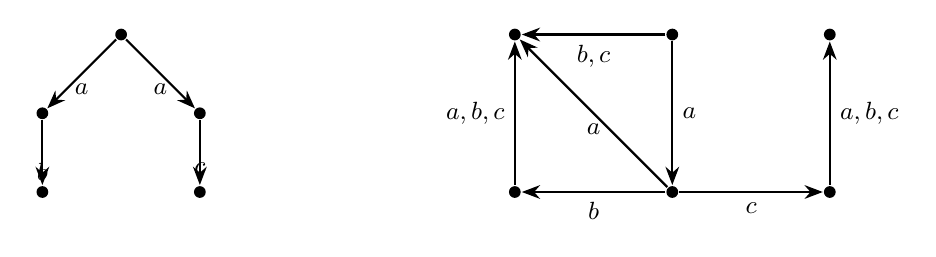
\begin{tikzpicture}[->, >=Stealth, node distance=2cm, thick, 
    main/.style = {draw, ellipse}, 
    dot/.style = {circle, fill, inner sep=1.5pt}]
    % Nodes

    \node[dot] (4) at (0, 0) {};
    \node[dot] (5) at (-1, -1) {};
    \node[dot] (6) at (1, -1) {};
    \node[dot] (7) at (-1, -2) {};
    \node[dot] (8) at (1, -2) {};


    \node[dot] (11) at (5, 0) {};
    \node[dot] (12) at (5, -2) {};
    \node[dot] (13) at (7, 0) {};
    \node[dot] (14) at (7, -2) {};
    \node[dot] (15) at (9, -2) {};
    \node[dot] (16) at (9, 0) {};

    % Edges
  

    \draw  (4) to node[midway, below] {\small$a$} (5) ;
    \draw  (5) to node[midway, below] {\small$b$} (7) ;
    \draw  (4) to node[midway, below] {\small$a$} (6) ;
    \draw  (6) to node[midway, below] {\small$c$} (8) ;


    \draw  (13) to node[midway, right] {\small$a$} (14) ;
    \draw  (14) to node[midway, below] {\small$b$} (12) ;
    \draw  (12) to node[midway, left] {\small$a,b,c$} (11) ;
    \draw  (13) to node[midway, below] {\small$b,c$} (11) ;
    \draw  (14) to node[midway, below] {\small$a$} (11) ;
    \draw  (14) to node[midway, below] {\small$c$} (15) ;
    \draw  (15) to node[midway, right] {\small$a,b,c$} (16) ;
    
    

\end{tikzpicture}
 \end{center}
    
\end{example}


\begin{definition}[$\HMLlin$]
    The fragment $\HMLlin^\exists$ of $\HML$ is characterized by the grammar
    \begin{align*}
        \varphi \Coloneqq true \; \mid \; \bev{a} \varphi        
    \end{align*}
    The fragment $\HML _{lin}^\forall$ is defined analogously. 
\end{definition}


\begin{example}
    Below an example of comparing bisimulation and linear equivalence
    \begin{center}
    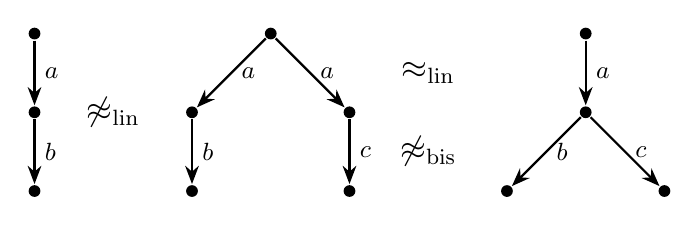
\begin{tikzpicture}[->, >=Stealth, node distance=2cm, thick, 
    main/.style = {draw, ellipse}, 
    dot/.style = {circle, fill, inner sep=1.5pt}]
    % Nodes

    \node[dot] (1) at (0, 0) {};
    \node[dot] (2) at (0, -1) {};
    \node[dot] (3) at (0, -2) {};


    \node (b) at (1,-1) {\large$\not\equlin$};
  
    
    \node[dot] (4) at (3, 0) {};
    \node[dot] (5) at (2, -1) {};
    \node[dot] (6) at (4, -1) {};
    \node[dot] (7) at (2, -2) {};
    \node[dot] (8) at (4, -2) {};

    \node (b) at (5,-0.5) {\large$\equlin$};
    \node (b) at (5,-1.5) {\large$\not\equbis$};
        
    \node[dot] (9) at (7, 0) {};
    \node[dot] (10) at (7, -1) {};
    \node[dot] (11) at (6, -2) {};
    \node[dot] (12) at (8, -2) {};
   

    % Edges
  
    \draw  (1) to node[midway, right] {\small$a$} (2) ;
    \draw  (2) to node[midway, right] {\small$b$} (3) ;
    
    \draw  (4) to node[midway, right] {\small$a$} (5) ;
    \draw  (5) to node[midway, right] {\small$b$} (7) ;

    \draw  (4) to node[midway, right] {\small$a$} (6) ;
    \draw  (6) to node[midway, right] {\small$c$} (8) ;

    \draw  (9) to node[midway, right] {\small$a$} (10) ;
    \draw  (10) to node[midway, right] {\small$b$} (11) ;
    \draw  (10) to node[midway, right] {\small$c$} (12) ;
    
    

\end{tikzpicture}
 \end{center}
\end{example}

% \begin{theorem}
%     $s \equbis t$ iff after Algorithm~\ref{alg:bis} terminates, either $s,t \in \sigma$, or $s,t \notin \sigma$. $s \equsim t$ iff after Algorithm~\ref{alg:sim} terminates, either $s,t \in \sigma$, or $s,t \notin \sigma$. 
% \end{theorem}



% \subsection{Logical charcterization}

% \begin{definition}[Hennessy-Milner Logic ($\HML$)]
%     Syntax: $\varphi = true\ |\ false\ |\ \varphi \land \varphi\ |\ \varphi \lor \varphi\ |\ \bev{a} \varphi\ |\ \bal{a} \varphi$, where $a \in A$.
    
%     Semantics: 
%     \begin{itemize}
%         \item $\T = (S, \to)$
%         \item $s \in S$
%         \item $\llbracket \varphi \rrbracket _\T \subseteq S$
%         \item $S \vDash _\T \varphi_1 \land \varphi_2$ iff $S \vDash_\T \varphi_1$ and $S \vDash _\T \varphi_2$
%         \item $S \vDash _\T \varphi_1 \lor \varphi_2$ iff $S \vDash_\T \varphi_1$ or $S \vDash _\T \varphi_2$
%         \item $S \vDash _\T \bev{a} \varphi$ iff $\exists s' \in \post_a(s).\ s' \vDash_\T \varphi$
%         \item $S \vDash _\T [ {a} ] \varphi$ iff $\forall s' \in \post_a(s).\ s' \vDash_\T \varphi$
%         \item $\llbracket true \rrbracket _\T = S$
%         \item $\llbracket false \rrbracket _\T = \varphi$
%         \item $\llbracket \varphi_1 \land \varphi_2 \rrbracket _\T = \llbracket \varphi_1 \rrbracket _\T \cap \llbracket \varphi_2 \rrbracket _\T$
%         \item $\llbracket \varphi_1 \lor \varphi_2 \rrbracket _\T = \llbracket \varphi_1 \rrbracket _\T \cup \llbracket \varphi_2 \rrbracket _\T$
%     \end{itemize}
% \end{definition}

% \begin{definition}
   
% \end{definition}

% \begin{theorem}
%     $s \equbis t$ iff $\forall \varphi \in \HML$, either $s,t \vDash \varphi$ or $s,t \nvDash \varphi$. $s \equsim t$ iff $\forall \varphi \in \HML ^\exists$, either $s,t \vDash \varphi$ or $s,t \nvDash \varphi$, iff $\forall \varphi \in \HML ^\forall$, either $s,t \vDash \varphi$ or $s,t \nvDash \varphi$. 
% \end{theorem}

% \section{State equivalence language (or trace) equivalence}

% Semantics:
% \begin{itemize}
%     \item $\T = (S, \to)$
%     \item $s \in S$
%     \item $L_\T = \{ a_1a_2\cdots a_n | \exists s_0 \cdots s_n.\ s_0 \stackrel {a_1} \to s_1 \stackrel {a_2} \to \cdots \stackrel {a_n} \to s_n \land s_0 = s \}$
% \end{itemize}

% \begin{lemma}
%     $L_\T(s)$ contains $\varepsilon$ and is prefix-closed.
% \end{lemma}

% \begin{definition}
%     $s_1 \approx_{lin} s_2$ iff $L_\T (s_1) = L_\T (s_2)$.
% \end{definition}

% \begin{remark}
%     $s_1 \equsim s_2$ implies $s_1 \approx_{lin} s_2$. (but not the other direction)
% \end{remark}

% To decide whether $L_{\T_1}(s) = L_{\T_2}(s)$, we decide whether $L_{\T_1}(s) \subseteq L_{\T_2}(s)$ and $L_{\T_2}(s) \subseteq L_{\T_1}(s)$. 

% \begin{remark}
%     $L_1 \subseteq L_2$ iff $L_1 \cap A^\star \setminus L_2 = \empty$. In total, this is PSPACE-hard.
% \end{remark}

% \begin{definition}[$\HML _{lin} ^\exists$]
%      $\varphi := true\ |\ \bev{a} \varphi$.
% \end{definition}

%
%% \newpage
% \bibliographystyle{plainnat}
% %\bibliographystyle{myplainnat} %a bit nicer for arxiv, revert to plainnat once bib is polished
% {\small
% \bibliography{reference}
% }




\begin{remark}
    To summarize:
    \begin{align*}
        \equiso &&  \mathrm{NP} && -\\
        \equbis && O(m log n) && \HML\\
        \equsim && O(m \cdot n) && \HML^{\exists}\\
         \equlin && \mathrm{PSPACE} && \HMLlin^{\exists}\\
    \end{align*}
\end{remark}
% \begin{itemize}
% 	\item $\approx_{iso} \to NP \to HML$.
% 	\item $\approx_{bis} \to O(m log n) \to HML^\exists$. (gfp)
% 	\item $\approx_{sim} \to O(m n) \to HML_{lin}^\exists$. (gfp)
% 	\item $\approx_{lin} \to pspace$.
% 	\item $[a](\varphi \land \psi) = [a]\varphi \land [a]\psi$
% 	\item $<a>(\varphi \lor \psi) = <a>\varphi \lor <a>\psi$
% 	\item $[\{a, b\}] \varphi = [a] \varphi \land [b] \varphi$
% 	\item $<\{a, b\}> \varphi = <a> \varphi \lor <b> \varphi$
% \end{itemize}

\section{Modal $\lmu$-calculus}

\begin{definition}[Modal $\lmu$-calculus Syntax]
    The syntax of the modal $\lmu$-calculus is defined by the following grammar. Let $X$ be a set of variables
    \begin{align*}
        \varphi \Coloneqq \HML \; \mid \;  x \in X \; \mid \; \underbrace{ \lmu x. \varphi}_{\lfp} \; \mid \;  \underbrace{\lnu x. \varphi}_{\gfp}
    \end{align*}
\end{definition}

\begin{definition}[Modal $\lmu$-calculus Semantics]
    The semantics of the modal $\lmu$-calculus is defined as follows.
    Let $T\coloneqq (S,\to)$ be a LTS over a finite action set (alphabet) $A$.
    The we define: (i) $ \eval{\varphi}_T^\interp \subseteq S$ where $\interp \colon X \to 2^S$; 
    (ii) $\eval{x}_T^\interp  = \interp(x)$; 
    (iii)  $\eval{\lmu x. \varphi}_T^\interp  = \bigcup_{\sigma \subseteq S} \eval{\varphi}_T^{\interp[x \to \sigma]}$; (iv) $\eval{\lnu x. \varphi}_T^\interp  = \bigcap_{\sigma \subseteq S} \eval{\varphi}_T^{\interp[x \to \sigma]}$.
\end{definition}

\begin{remark}
        Let $F\coloneqq \lambda \sigma \subseteq S.\eval{\varphi}_T^{\interp[x \to \sigma]}$ then
    $\eval{\lmu x. \varphi}_T^\interp = \lfp F$ and $\eval{\lnu x. \varphi}_T^\interp = \gfp F$.
    That is, $\lfp F$ is the limit (infinite union) of 
    \begin{align*}
        \sigma_0 = \emptyset 
        \subseteq \sigma_1 = \eval{\varphi}_T^{\interp[x \to \sigma_0]}
        \subseteq  \sigma_2 = \eval{\varphi}_T^{\interp[x \to \sigma_1]} 
        \subseteq \cdots
    \end{align*}
    and $\lfp F$ is the limit (infinite intersection) of 
    \begin{align*}
        \sigma_0 = S
        \supseteq \sigma_1 = \eval{\varphi}_T^{\interp[x \to \sigma_0]}
        \supseteq  \sigma_2 = \eval{\varphi}_T^{\interp[x \to \sigma_1]} 
        \supseteq \cdots
    \end{align*}
\end{remark}

\begin{example}
    Consider the expression $(\lmu x)(\bev{a} \true \lor \bev{\bar{a}}x)$ where $\bar{a}\coloneqq A\setminus \{a\}$. By evaluating the expression we obtain
    \begin{align*}
        \sigma_0 &= \false \\
        \sigma_1 &= \bev{a}\true \\
        \sigma_2 &= \bev{a}\true  \lor \bev{\bar{a}}\bev{a}\true \\
        \sigma_3 &= \bev{a}\true  \lor \bev{\bar{a}} (\bev{a}\true  \lor \bev{\bar{a}}\bev{a}\true)\\
        &= \bev{a}\true  \lor \bev{\bar{a}}\bev{a}\true \lor \bev{\bar{a}}\bev{\bar{a}}\bev{a}\true\\
        \sigma_4 &= \cdots
    \end{align*}
    It expresses that 
    there exists a path somewhere along the path there exists an $a$-transition, i.e., $\exists \lev a$. 
\end{example}

\begin{example}
    Consider the expression $(\lnu x)(\bal{\bar{a}} \false \land \bev{a}x)$. By evaluating the expression we obtain
    \begin{align*}
        \sigma_0 &= \true \\
        \sigma_1 &= \bal{\bar{a}}\false \\
        \sigma_2 &= \bal{\bar{a}}\false \land \bal{a}\bal{\bar{a}}\false \\
        \sigma_3 &= \cdots
    \end{align*}
    It expresses that 
    on all paths there are only $a$-transition, i.e., $\forall \lal a$. 
\end{example}

\begin{remark}
 The the equivalence $\neg \lmu x. \varphi(x) = \lnu x . \neg \varphi (\neg x)$ where left has even number of negations.
\end{remark}



\begin{definition}[$\lmu$-calculus]
We can add propositions $p\in P$ as atomic formulas. Syntactically we can define the grammar
 \begin{align*}
        \varphi \Coloneqq p \; \mid \; \varphi \lor \varphi\; \mid \;  \varphi \land \varphi \; \mid \;  \bev{a}\varphi  \; \mid \; \bal{a}\varphi  \; \mid \;  \lmu x. \varphi \; \mid \; \lnu x. \varphi x
\end{align*}
    Semantically we evaluate over Kripke structures, i.e., $K=(S, \to, \eval{\cdot}\colon S\to 2^P)$, e.g., $\eval{p}_K\subseteq S$
\end{definition}

\begin{remark}
    We can formulate the following abbreviations:
    \begin{align*}
        \exists \lev \varphi &= \lmu x. (\varphi \lor \exists \lne x) \\
        \exists \lev p &= \lmu x. (p \lor \exists \lne x) & \quad \text{($p$ is reachable)} \\
         \forall \lal \varphi &= \lnu x. (\varphi \land \forall \lne x) \\
         \forall \lal p &= \lnu x. (p \land \forall \lne x)  & \quad \text{($p$ is an invariant)}  \\
         \forall \lev \varphi &= \lmu x. (\varphi \lor \forall \lne x) & \quad \text{(on all paths $\varphi$ is eventually true)} \\
          \exists \lev \varphi &= \lnu x. (\varphi \land \exists \lne x) & \quad \text{(there exists an inf.\ path where $\varphi$ is always true)} 
    \end{align*}
\end{remark}


% 	\item
% 	\item $\lmu$-calculus add propositions as atomic formulas i.e. $\varphi := p | \varphi \lor \varphi | \varphi \land \varphi | <a> \varphi | [a] \varphi | \lmu x.\varphi | \lnu x.\varphi | X$
% 	\item $\llbracket p\rrbracket_T \subset S$
% 	\item LTS $T = (S, \to) $ Kripke structure $K = (S, \to, \llbracket\rrbracket:S \to 2^P)$
% \end{itemize}

% Abbreviations:
% \begin{itemize}
% 	\item $\exists \lev \varphi = \lmu x. (\varphi \lor \exists \lne x)$
% 	\item $\exists \lev p = \lmu x. (p \lor \exists \lne x)$ i.e. p is reachable.
% 	\item $\forall \lal \varphi = \lnu x. (\varphi \land \forall \lne x)$
% 	\item $\forall \lal p = \lnu x. (p \land \forall \lne x)$ i.e. p is an invariant.
% 	\item $\forall \lev \varphi = \lmu x. (\varphi \lor \forall \lne x)$
% 	\item $\exists \lal \varphi = \lnu x. (\varphi \land \exists \lne x)$ i.e. there exists an infinite path along which $\varphi$ is always true.
% \end{itemize}
% equivalant to
% $$\llbracket \lmu x \varphi \rrbracket_T^I = \text{lfp}(F)$$
% for 
% $$F = \lambda \sigma \subset S. \llbracket\varphi \rrbracket_T^{I[x \to \sigma]}$$
% $\text{lfp}(F)$ is the limit (inf union) of:
% $$\sigma_0 = \varnothing$$
% $$\subseteq \sigma_1 = \llbracket\varphi \rrbracket_T^{I[x \to \sigma_0]}$$
% $$\subseteq \sigma_2 = \llbracket\varphi \rrbracket_T^{I[x \to \sigma_1]}$$
% $$\dots$$
% $$\subseteq S$$

% And same for $\lnu$:
% $$\llbracket \lnu x \varphi \rrbracket_T^I = \cap_{\sigma \subset S} \llbracket\varphi \rrbracket_T^{I[x \to \sigma]}$$
% equivalant to
% $$\llbracket \lnu x \varphi \rrbracket_T^I = \text{gfp}(F)$$
% for 
% $$F = \lambda \sigma \subset S. \llbracket\varphi \rrbracket_T^{I[x \to \sigma]}$$
% $\text{gfp}(F)$ is the limit (inf intersection) of:
% $$\sigma_0 = S$$
% $$\supseteq \sigma_1 = \llbracket\varphi \rrbracket_T^{I[x \to \sigma_0]}$$
% $$\supseteq \sigma_2 = \llbracket\varphi \rrbracket_T^{I[x \to \sigma_1]}$$
% $$\dots$$


% \begin{example}
% $$\lmu x . (<a> true \lor <\bar{a}> x)$$
% solution:
% $$\sigma_0 = false$$
% $$\sigma_1 = <a> true$$
% $$\sigma_2 = <a> true \lor <\bar{ a}><a>true$$
% $$\sigma_3 = <a> true \lor <\bar{ a}>(<a>true \lor <\bar{ a}><a>true)$$
% $$= <a> true \lor <\bar{ a}><a>true \lor <\bar{ a}><\bar{ a}><a>true$$
% $$\sigma_4 = \dots$$

% means "$\exists \lev a$"
% there exists a path somewhere along the path there exists an a transition.

% \end{example}

% \begin{example}
% $$(\lnu x)([\bar{ a}] flase \land [a] x)$$
% solution:
% $$\sigma_0 = true$$
% $$\sigma_1 = [\bar{ a}]false \land [a]true$$
% $$\sigma_2 = [\bar{ a}]false \land [a][\bar{ a}]false$$
% $$\sigma_3 = \dots$$

% means  "$\forall \lal a$" 
% on all paths only a transitions.
% \end{example}

% Some notes:
% \begin{itemize}
% 	\item $\neg \lmu x. \varphi(x) = \lnu x . \neg \varphi (\neg x)$ where left has even number of negations.
% 	\item $\lmu$-calculus add propositions as atomic formulas i.e. $\varphi := p | \varphi \lor \varphi | \varphi \land \varphi | <a> \varphi | [a] \varphi | \lmu x.\varphi | \lnu x.\varphi | X$
% 	\item $\llbracket p\rrbracket_T \subset S$
% 	\item LTS $T = (S, \to) $ Kripke structure $K = (S, \to, \llbracket\rrbracket:S \to 2^P)$
% \end{itemize}

% Abbreviations:
% \begin{itemize}
% 	\item $\exists \lev \varphi = \lmu x. (\varphi \lor \exists \lne x)$
% 	\item $\exists \lev p = \lmu x. (p \lor \exists \lne x)$ i.e. p is reachable.
% 	\item $\forall \lal \varphi = \lnu x. (\varphi \land \forall \lne x)$
% 	\item $\forall \lal p = \lnu x. (p \land \forall \lne x)$ i.e. p is an invariant.
% 	\item $\forall \lev \varphi = \lmu x. (\varphi \lor \forall \lne x)$
% 	\item $\exists \lal \varphi = \lnu x. (\varphi \land \exists \lne x)$ i.e. there exists an infinite path along which $\varphi$ is always true.
% \end{itemize}

\subsection{Computational Tree Logic (CTL)}

\begin{definition}[CTL Syntax]
    The syntax of the Computation Tree Logic (CTL) is given by the following grammar
    \begin{align*}
        \varphi \Coloneqq p \;\mid\; 
        \varphi \lor \varphi \;\mid\; 
        \varphi \land \varphi \;\mid\; 
        \overbrace{\exists \lne \varphi}^{EX} \;\mid\; 
        \overbrace{\forall \lne \varphi}^{AX} \;\mid\;
        \overbrace{\exists \lev \varphi}^{EF} \;\mid\;
        \overbrace{\forall \lev \varphi}^{AF} \;\mid\; 
        \overbrace{\exists \lal \varphi}^{EG} \;\mid\;
        \overbrace{\forall \lal \varphi}^{AG}
    \end{align*}
\end{definition}

\begin{remark}
    The following equivalences hold: $\exists \lne \varphi = \neg \forall \lne \neg \varphi$ and $\exists \lev \varphi = \neg \forall \lal \neg \varphi$.
\end{remark}

\begin{remark}
    The full $\lmu$-calculus is strictly more expressive than CTL, in two ways: (i) $\lmu x.\exists \lne \exists \lne x$ means $p$ is reachable in even number of steps. (ii) $\lnu x. \exists \lev (p \land \exists \lne x) = \lnu x .\, \lmu y ((p \land \exists \lne x) \lor \exists \lne y)$ means there exists a path with infinitely many $p$ clauses. It is not expressible in CTL.
\end{remark}

\begin{exercise}
    Proof that $\lmu x.\exists \lne \exists \lne x$ is not expressible in CTL.
\end{exercise}


\begin{remark}
    We have that $\forall \lal \forall \lev p = \forall \lal \lev p$ expresses that on all infinite paths, we have $p$ infinitely often. 
     By contrast, while
     $\exists \lal \exists \lev p \Leftarrow  \exists \lal \lev p$ the reverse does not hold, e.g.,
     \begin{center}
		\begin{tikzpicture}
			\node (S) at (10,11) {};
			\node[circle,draw, minimum size= 0.7cm, inner sep=1.5pt] (A) at (10,10) {\small$\neg p$};
			\node[circle,draw, minimum size= 0.7cm, inner sep=1.5pt] (B) at (12,10) {\small$p$};
			\path[->]
			(S) edge (A)
			(A) edge (B)
			(A) edge [out=135, in=225, loop] (A);
			%\draw[->] (w0) -- (w1);
		\end{tikzpicture}
	\end{center}
 Moreover, $CTL$ characterizes $\equbis$ and  $CTL^\exists$ characterizes $\equsim$.
 Next we define a logic that characterizes $\equlin$.
\end{remark}



\subsection{Linear Temporal Logic (LTL)}

\begin{remark}
    LTL characterizes $\equlin$.
\end{remark}


\begin{definition}[LTL Snytax]
    The syntax of Linear Temporal Logic (LTL) is given by the following grammar
    \begin{align*}
        phi \Coloneqq p \;\mid\;  
        \varphi \lor \varphi \;\mid\; 
        \varphi \land \varphi \;\mid\; 
        \lne \varphi \;\mid\;  
        \lev \varphi 
        \;\mid\; \lal \varphi
    \end{align*}
\end{definition}

\begin{definition}[LTL Semantics]
LTL is interpreted over inf traces $t = s_0s_1s_2s_3\dots$ s.t $s_i \to s_{i+1}$ for all $i \geq 0$ the we define 
\begin{align*} 
&t \models p &\iff \quad&p \in \eval{s_0} & \\
&t \models \lne \varphi &\iff \quad&s_0s_1s_2s_3\dots \models \varphi & \quad \text{next $\varphi$}\\
&t \models \lev \varphi &\iff \quad&\exists i\geq0 s_is_{i+1}s_{i+2}s_{i+3}\dots \models \varphi & \quad \text{eventually $\varphi$}\\
&t \models \lal \varphi &\iff \quad&\forall i\geq0 s_is_{i+1}s_{i+2}s_{i+3}\dots \models \varphi & \quad \text{always $\varphi$}\\
\end{align*}
We say $s \models \varphi$ iff there exists trace $t$ from $s$ s.t. $t \models \varphi$.
\end{definition}

\begin{remark}
    Now you can compare LTL to CLT etc. For example $\lal \lev p$ is infinitely often $p$. It is incomparable to CTL (fragment of of $\lmu$-calculus).
% This logic was defined as a first order logic, but we should also add until operator to it to be complete with respect to first order logic.
\end{remark}

\begin{definition}[Until]
We define the until operator $\lun$ as 
\begin{align*}
    \varphi\lun\psi \iff \exists s_is_{i+1}\dots \models \psi \land \forall j<i. s_js_{j+1}\dots\models \varphi
\end{align*}
\end{definition}

% \begin{itemize}
% 	\item $t \models p$ iff $p \in \llbracket s_0\rrbracket$
% 	\item $t \models \lne \varphi$ iff $s_1s_2s_3\dots \models \varphi$. next
% 	\item $t \models \lev \varphi$ iff $\exists i\geq0 s_is_{i+1}s_{i+2}s_{i+3}\dots \models \varphi$. eventually
% 	\item $t \models \lal \varphi$ iff $\forall i\geq0 s_is_{i+1}s_{i+2}s_{i+3}\dots \models \varphi$ always
% \end{itemize}
% We say $s \models \varphi$ iff there exists trace $t$ from $s$ s.t. $t \models \varphi$.


% Now you can compare LTL to CLT etc. For example $\lal \lev p$ is inf often p. It is not comparable to CTL, fragment of of $\lmu$-calculus.

% This logic was defined as a first order logic, but we should also add until operator to it to be complete with respect to first order logic.







% \renewcommand{\implies}{\Rightarrow}
% \newcommand{\implied}{\Leftarrow}
% \newcommand{\eps}{\varepsilon}
% \newcommand{\defas}{\coloneqq}
% \renewcommand{\le}{\sqsubseteq}
% \renewcommand{\ge}{\sqsupseteq}
% \renewcommand{\sqcap}{\bigsqcap}
% \renewcommand{\sqcup}{\bigsqcup}
% \newcommand{\bottom}{\perp}


% \newcommand{\Theorem}[2][]{\begin{theorem}[#1]#2\end{theorem}}
% \newcommand{\Definition}[2][]{\begin{definition}[#1]#2\end{definition}}
% \newcommand{\Example}[2][]{\begin{example}[#1]#2\end{example}}
% \newcommand{\Homework}[2][]{\begin{homework}[#1]#2\end{homework}}
% \newcommand{\Lemma}[2][]{\begin{lemma}[#1]#2\end{lemma}}
% \newcommand{\Remark}[2][]{\begin{remark}[#1]#2\end{remark}}
% \newcommand{\Figure}[1]{\begin{figure}#1\end{figure}}
% \newcommand{\Itemize}[1]{\begin{itemize}#1\end{itemize}}
% \newcommand{\Enumerate}[1]{\begin{enumerate}#1\end{enumerate}}



% \chapter{Class 22}

\section{Concurrency Theory}

\begin{remark}
    Calculus of Communicating Systems (CCS) can be given two semantics.
\begin{itemize}
\item \emph{Sequential semantics:} 
		Labeled transition systems and logics (e.g., Hennessy-Milner logic (HML) and temporal logic)
\item \emph{Truly concurrent semantics:} 
        Petri Nets (because parallelism is different from nondeterminism)
\end{itemize}
\end{remark}


\begin{definition}[Petri nets]
A \emph{petri net} is a tuple $N = (P, T)$ where $P$ is a set of places and $T$ a set of transitions.
	The state of a petri net is given by a marking $M \colon P \to \NN$ and a transition is a function that takes a marking and an action and returns another marking, i.e., $t \colon M \to M$.
	Equivalently, considering a set of names for each transition (actions) $A$, we have that $T \colon M \times A \to M$.
\end{definition}



\begin{remark}[Petri nets as lebeled transition systems]
    A Petri net $N = (P, T)$ can be interpreted as the following labeled transition system (LTS) $LTS_N = (M, \to)$.
	The transition $\to$ is given by $m \to m'$ if and only if there exists $t \in T$ such that: (i) the transformation $t$ decomposes in precodition $^*t \in M$, action $a \in A$ and postcondition $t^* \in M$, i.e., $t = (^\bullet t, a, t^\bullet)$; 
 (ii) the precodition $^\bullet t$ is contained in $m$, i.e., $^\bullet t \subseteq m$; 
 (iii) the transformation $t$ converts $m$ into $m'$, i.e., $m' = m - ^\bullet t + t^\bullet$.
\end{remark}

\begin{example}[Petri net]
    Consider the Petri net $N = (P, T)$ where $P = \{ p_1, p_2, p_3, p_4, p_5 \}$, $T = \{ t \}$, and $t \colon \{ (p_1, 2), (p_2, 1) \} \mapsto \{ (p_4, 1), (p_5, 1) \}$.
	In other words, $t$ can fire a transition if there are $2$ markings in $p_1$ and $1$ marking in $p_2$, and adds $1$ marking in $p_4$ and $1$ marking in $p_5$.  
    \begin{center}
        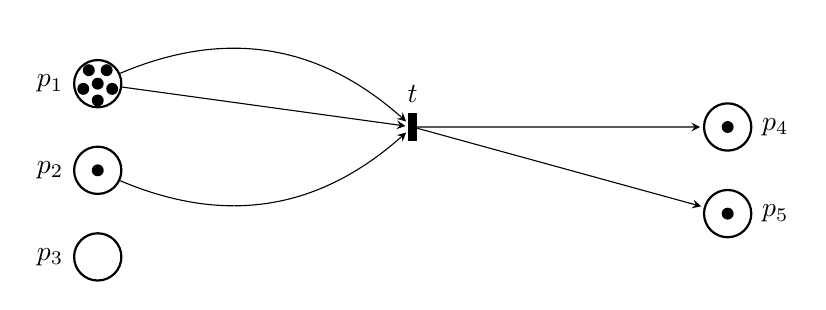
\begin{tikzpicture}[
		yscale=-1.1,
		thin,
		>=stealth,
  		every transition/.style={fill,minimum width=1mm,minimum height=3.5mm},
  		every place/.style={draw,thick,minimum size=6mm}
	]

		% Places
		\node[place,label=left:$p_1$] (p1) at (0, 1) {};    
		\node[place,label=left:$p_2$] (p2) at (0, 2) {};    
		\node[place,label=left:$p_3$] (p3) at (0, 3) {};    
		\node[place,label=right:$p_4$] (p4) at (8, 1.5) {};    
		\node[place,label=right:$p_5$] (p5) at (8, 2.5) {};  

		% Tokens
		\node[token, tokens=5] at (p1) {}; 
		\node[token] at (p2) {};
		\node[token] at (p4) {};  
		\node[token] at (p5) {};  

		% Transitions
		\node[transition, label=above:$t$] at (4, 1.5) {}  
			edge[] [pre] (p1) 
			edge[bend left] [pre] (p1) 
			edge[bend right] [pre] (p2) 
			edge [post] (p4)
			edge [post] (p5);
	\end{tikzpicture}
    \end{center}
\end{example}





\begin{definition}[Sequential net]
	A Petri net is \emph{sequential} if all transformations $t$ have a precondition $^*t$ such that $|^*t| \le 1$.
	Sequential nets are equivalent to regular languages for finite strings. 
    
\end{definition}

\begin{example}[Sequential net]
    Below an example of a sequential net.
    \begin{center}
        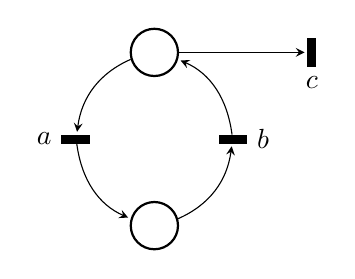
\begin{tikzpicture}[
		yscale=-1.1,
		thin,
		>=stealth,
  		every transition/.style={fill,minimum width=1mm,minimum height=3.5mm},
  		every place/.style={draw,thick,minimum size=6mm}
	]

		% Places
		\node[place] (p1) at (1, 0) {};    
		\node[place] (p2) at (1, 2) {};

		% Transitions
		\node[transition, label=left:$a$, style={fill,minimum width=3.5mm,minimum height=1mm}] at (0, 1) {}  
			edge[bend right] [pre] (p1)
			edge[bend left] [post] (p2);
		\node[transition, label=right:$b$, style={fill,minimum width=3.5mm,minimum height=1mm}] at (2, 1) {}  
			edge[bend right] [pre] (p2)
			edge[bend left] [post] (p1);
		\node[transition, label=below:$c$] at (3, 0) {}  
			edge[] [pre] (p1);
	\end{tikzpicture}
    \end{center}
\end{example}





\begin{definition}[Basic parallel process]
	A Petri net is a \emph{basic parallel processes} if all transformations $t$ have a precondition $^*t$ such that $|^*t| = 1$.
	Basic parallel processes are equivalent to context-free languages for finite strings. 
\end{definition}

\begin{example}[Basic parallel process]
     Below an example of a basic parallel process.
     \begin{center}
         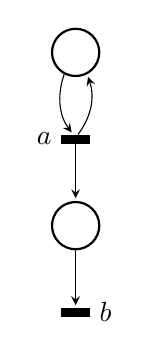
\begin{tikzpicture}[
		yscale=-1.1,
		thin,
		>=stealth,
  		every transition/.style={fill,minimum width=3.5mm,minimum height=1mm},
  		every place/.style={draw,thick,minimum size=6mm}
	]

		% Places
		\node[place] (p1) at (0, 0) {};    
		\node[place] (p2) at (0, 2) {};

		% Transitions
		\node[transition, label=left:$a$] at (0, 1) {}  
			edge[bend right] [pre] (p1)
			edge[] [post] (p2)
			edge[bend left] [post] (p1);
		\node[transition, label=right:$b$] at (0, 3) {}  
			edge[] [pre] (p2);
	\end{tikzpicture}
     \end{center}
\end{example}


\begin{definition}[Chomsky hierarchy]
	The \emph{Chomsky hierarchy} is a hierarchy of sequential computation given by
 \begin{align*}
     FA 
			\subseteq PDA
			\subseteq LBA
			\subseteq TM \,,
 \end{align*}
	where the decidabilities are as follows.
 \begin{itemize}
        \item FA. Fully decidable.
		\item PDA. Universality is undecidable, i.e., $L(A) \stackrel{?}{=} \Sigma^*$.
		\item LBA. Emptyness is undecidable, i.e., $L(A) \stackrel{?}{=} \emptyset$.
		\item TM. Membership is undecidable, i.e., $w \stackrel{?}{\in} L(A)$.
 \end{itemize}
\end{definition}

\begin{definition}[Concurrency hierarchy] 
	The \emph{concurrency hierarchy} is a hierarchy of concurrent computation given by
 \begin{align*}
     FA 
			\subseteq BPP
			\subseteq CCS
			\subseteq TM \,,
 \end{align*}
	where, in CCS, reachability is decidable but non-elementary.
\end{definition}


\begin{exercise}[Ortogonal Hierarchies]
    Solve the following tasks.
    \begin{enumerate}[(i)]
      \item Show that $X = a (X | b) + c (X | d) + e$ is not context-free.
		Hint: use the pumping lemma.

		\item Present a context-free language that is not in BPP, and try to prove it. 

    		\item Give a Petri net that generates $\{ a^n b^n | n > 0 \}$.
    \end{enumerate}
\end{exercise}


\begin{definition}[Coverage problem for Petri nets]
	Given a Petrin net $N$ and two marking $m, m'$, the problem is to decide the existence of a sequence of transitions that take $m$ to a marking that covers $m'$, i.e., if there exists $m''$ such that $m \to^* m''$ and $m' \subseteq m''$.
     As opposed to the reachability question, the coverage problem asks for $m' \subseteq m''$ instead of $m' = m''$.
\end{definition}


\begin{remark}
    The coverage problem is a finite problem, since every finite Petri net $N$ has a finite coverage tree of size $\mathcal{O}(n^n)$ where $n = |N|$.
The coverage tree can be obtained by the Karp-Miller algorithm, which generates a tree of depth at most $\mathcal{O}(n \log n)$.
\end{remark}

\begin{example}
    Consider the Petri net with an initial marking is given below.
\begin{center}
    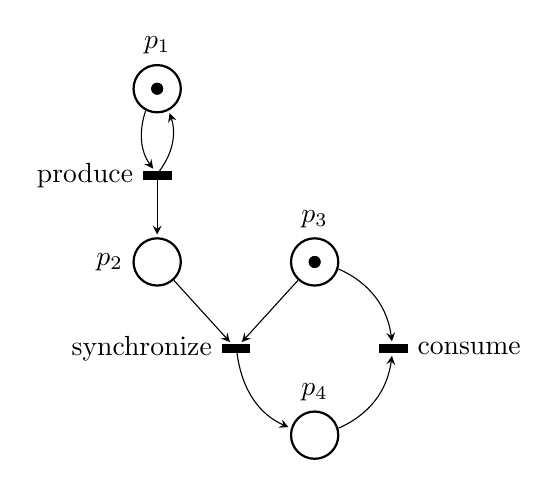
\begin{tikzpicture}[
		yscale=-1.1,
		thin,
		>=stealth,
  		every transition/.style={fill,minimum width=3.5mm,minimum height=1mm},
  		every place/.style={draw,thick,minimum size=6mm}
	]

		% Places
		\node[place, label=above:$p_1$] (p1) at (0, 0) {};    
		\node[place, label=left:$p_2$] (p2) at (0, 2) {};   
		\node[place, label=above:$p_3$] (p3) at (2, 2) {};   
		\node[place, label=above:$p_4$] (p4) at (2, 4) {};

		% Tokens
		\node[token, tokens=1] at (p1) {}; 
		\node[token, tokens=1] at (p3) {};

		% Transitions
		\node[transition, label=left:{produce}] at (0, 1) {}  
			edge[bend right] [pre] (p1)
			edge[bend left] [post] (p1)
			edge[] [post] (p2);
		\node[transition, label=left:{synchronize}] at (1, 3) {}  
			edge[] [pre] (p2)
			edge[] [pre] (p3)
			edge[bend left] [post] (p4);
		\node[transition, label=right:{consume}] at (3, 3) {}  
			edge[bend right] [pre] (p4)
			edge[bend left] [pre] (p3);
	\end{tikzpicture}
\end{center}
The corresponding coverage tree follows.
Note that $m'$ is covered by $m$ if there is a node in the tree that covers it. 
\begin{center}
    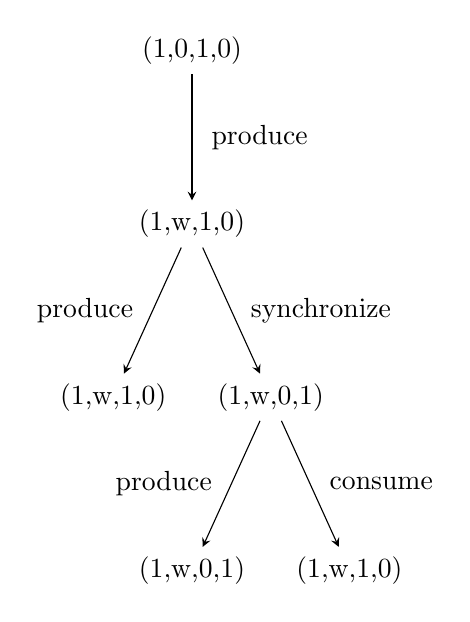
\begin{tikzpicture}[
		yscale=-1.1,
		thin,
		>=stealth,
	]

		% markings
		\node (a) at (0, 0) {(1,0,1,0)};
		\node (b) at (0, 2) {(1,w,1,0)};    
		\node (c) at (-1, 4) {(1,w,1,0)};   
		\node (d) at (1, 4) {(1,w,0,1)};
		\node (e) at (0, 6) {(1,w,0,1)};
		\node (f) at (2, 6) {(1,w,1,0)};

		% transformations
		\path [->] (a) edge node[label=right:{produce}] {} (b);
		\path [->] (b) edge node[label=left:{produce}] {} (c);
		\path [->] (b) edge node[label=right:{synchronize}] {} (d);
		\path [->] (d) edge node[label=left:{produce}] {} (e);
		\path [->] (d) edge node[label=right:{consume}] {} (f);
	\end{tikzpicture}
\end{center}

\end{example}

\begin{definition}[Control-flow models]
	Graphs whose nodes represent control states and whose edges represent control flow. 
	For example, labeled transition systems and Petri nets.
\end{definition}

\begin{definition}[Data-flow models]
	Also called circuits, they are graphs whose nodes represent actors (gates) and whose edges represent data flow. 
\end{definition}

\begin{example}
    Below an example of a data-flow model.
    \begin{center}
        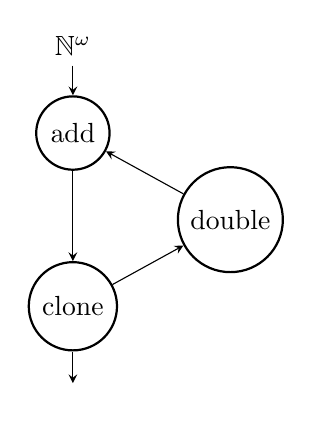
\begin{tikzpicture}[
		yscale=-1.1,
		thin,
		>=stealth,
	]

		% markings
		\node (input) at (0, 0) {$\NN^\omega$};
		\begin{scope}[every node/.style={circle,thick,draw}]
			\node (b) at (0, 1) {add};    
			\node (c) at (0, 3) {clone};   
			\node (d) at (2, 2) {double};
		\end{scope}
		\node (output) at (0, 4) {};

		% transformations
		\path [->] (input) edge node {} (b);
		\path [->] (b) edge node {} (c);
		\path [->] (c) edge node {} (d);
		\path [->] (d) edge node {} (b);
		\path [->] (c) edge node {} (output);
	\end{tikzpicture}
    \end{center}
\end{example}


% \Figure {
% 	\centering
% 	\begin{tikzpicture}[
% 		yscale=-1.1,
% 		thin,
% 		>=stealth,
% 	]

% 		% markings
% 		\node (input) at (0, 0) {$\NN^\omega$};
% 		\begin{scope}[every node/.style={circle,thick,draw}]
% 			\node (b) at (0, 1) {add};    
% 			\node (c) at (0, 3) {clone};   
% 			\node (d) at (2, 2) {double};
% 		\end{scope}
% 		\node (output) at (0, 4) {};

% 		% transformations
% 		\path [->] (input) edge node {} (b);
% 		\path [->] (b) edge node {} (c);
% 		\path [->] (c) edge node {} (d);
% 		\path [->] (d) edge node {} (b);
% 		\path [->] (c) edge node {} (output);
% 	\end{tikzpicture}
% 	\caption{Data-flow model example}
% 	\label{Figure: Data-flow model}
% }

\begin{definition}[Combinatorial circuits]
	A data-flow model is a \emph{combinatorial circuit} if there are no loops.
	For combinatorial circuits, every tuple of inputs produces a tuple of outputs.
\end{definition}

\begin{definition}[Sequential circuits] 
	A data-flow model is a \emph{sequential circuit} if there are loops.
	For sequential circuits, every sequence of inputs produces a sequence of outputs.
\end{definition}

\begin{remark}
    To deal with loops in sequential circuits, there are two approaches, i.e., 
    synchronous (clocked) and asynchronous (queues as channels -- Kahn networks).
\end{remark}






\printindex

\end{document}